% TouchSynth Poly design report
% build: python3 gen_tables.py && latexmk -pdf touchsynth_poly_report.tex   (in WSL; see the last appendix)
\documentclass[11pt,a4paper]{article}
\usepackage[T1]{fontenc}
\usepackage[utf8]{inputenc}
\usepackage{lmodern}
\usepackage{textcomp}
\usepackage{microtype}
\usepackage[a4paper,textwidth=16cm,top=2.5cm,bottom=2.7cm]{geometry}
\usepackage{graphicx}
\usepackage{booktabs,longtable,tabularx,array,multirow}
\usepackage{siunitx}
\usepackage{xcolor}
\usepackage{tikz}
\usetikzlibrary{positioning,arrows.meta,fit,calc,shapes.geometric,decorations.pathreplacing,patterns,backgrounds}
\usepackage[siunitx,american]{circuitikz}
\usepackage{pgfplots}
\pgfplotsset{compat=1.16}
\usepackage{caption,subcaption}
\usepackage{enumitem}
\usepackage{pdfpages}
\usepackage[section]{placeins}
\usepackage{fancyhdr}
\usepackage[hidelinks]{hyperref}

\hypersetup{pdftitle={TouchSynth Poly - design report}}
\graphicspath{{../figures/}}
\captionsetup{font=small,labelfont=bf}
\setlist{nosep,leftmargin=1.4em}
\sisetup{range-phrase=\,\ldots\,,range-units=single}
\newcommand{\file}[1]{\texttt{#1}}
\newcommand{\sub}[1]{\textsubscript{#1}}
\newcommand{\placeholder}[1]{\par\smallskip\noindent\fcolorbox{orange!70!black}{orange!8}{\parbox{0.97\linewidth}{%
  \small\textbf{Placeholder.} #1}}\par\smallskip}
% generated by gen_tables.py -- do not edit
\newcommand{\statVoiceParts}{190}
\newcommand{\statVoiceNets}{114}
\newcommand{\statVoiceSheets}{6}
\newcommand{\statBpParts}{201}
\newcommand{\statBpNets}{139}
\newcommand{\statBpSheets}{4}
\newcommand{\statVoiceAsm}{165}
\newcommand{\statVoiceLines}{49}
\newcommand{\statVoiceBasic}{32}
\newcommand{\statVoicePromo}{17}
\newcommand{\statVoiceCost}{3.01}
\newcommand{\statBpAsm}{153}
\newcommand{\statBpLines}{37}
\newcommand{\statBpBasic}{32}
\newcommand{\statBpPromo}{5}
\newcommand{\statBpCost}{6.21}
\newcommand{\statSystemCost}{30.29}
\newcommand{\statVoiceHand}{4}
\newcommand{\statVoiceDnp}{8}
\newcommand{\statVoiceTp}{13}
\newcommand{\statBpHand}{18}
\newcommand{\statBpDnp}{18}
\newcommand{\statBpTp}{12}
\newcommand{\statVoiceMcu}{CH32V006F8P7}
\newcommand{\statBpGpioFree}{3}
\newcommand{\statBpGpioUsed}{34}
\newcommand{\statVoiceSegments}{1786}
\newcommand{\statVoiceVias}{404}
\newcommand{\statVoiceFootprints}{190}
\newcommand{\statVoiceLenF}{1.43}
\newcommand{\statVoiceLenB}{1.01}
\newcommand{\statBpSegments}{1411}
\newcommand{\statBpVias}{1696}
\newcommand{\statBpGndVias}{1557}
\newcommand{\statBpLenF}{2.76}
\newcommand{\statBpLenB}{1.75}
\newcommand{\statSnineDacCseven}{$-$59.8}
\newcommand{\statStenFcLow}{19}
\newcommand{\statStenFcHigh}{30.4}
\newcommand{\statStenThd}{0.47}
\newcommand{\statStenSnrLo}{68.8}
\newcommand{\statStenSnrHi}{69.4}
\newcommand{\statStenCurrent}{4.0}
\newcommand{\statSelevenCarrier}{$-$74.1}
\newcommand{\statSelevenCarrierNone}{$-$41.6}
\newcommand{\statSelevenCarrierLow}{$-$38.9}
\newcommand{\statSelevenDroopTen}{$-$0.04}
\newcommand{\statSelevenDroopTwenty}{$-$0.79}
\newcommand{\statSelevenRmix}{243}
\newcommand{\statStwelveGain}{0.357}
\newcommand{\statStwelveHard}{3.95}
\newcommand{\statStwelveHardMargin}{1.96}
\newcommand{\statStwelveCentre}{2.79}
\newcommand{\statStwelveCentreMargin}{5.0}
\newcommand{\statStwelveSupply}{0.34}
\newcommand{\statStwelveVref}{2.41}
\newcommand{\statStwelveCardHard}{1.39}
\newcommand{\statStwelveCardUncapped}{1.95}
\newcommand{\statSthirteenSep}{48}
\newcommand{\statSthirteenCentre}{$-$3.5}
\newcommand{\statSthirteenThd}{0.47}
\newcommand{\statSthirteenSnr}{68.8}
\newcommand{\statSthirteenClick}{28}
\newcommand{\statSthirteenCurrent}{4.7}
\newcommand{\statSthirteenParts}{22}
\newcommand{\statBusMultiChord}{38}
\newcommand{\statBusChord}{87}


\pagestyle{fancy}
\fancyhf{}
\setlength{\headheight}{14pt}
\lhead{\small TouchSynth Poly -- design report}
\rhead{\small draft 0.1}
\cfoot{\small\thepage}

\title{\textbf{TouchSynth Poly}\\[4pt]\large A polyphonic analog synthesizer:\\ voice cards with digital oscillators
and analog filters on a USB backplane\\[10pt]\normalsize Design report, draft 0.1}
\author{}
\date{20 October 2026}

\begin{document}
\maketitle
\thispagestyle{empty}
\vspace{-2em}

\begin{abstract}
\noindent TouchSynth Poly is a polyphonic synthesizer with four to eight voices. Each voice is a plug-in card with its
own CH32V006 microcontroller. The firmware generates up to three band-limited oscillators (or a modal drum) and writes
them to a \SI{187.5}{kHz} PWM DAC. The analog part of the card follows TouchSynth rev 0.1, redesigned for a single
\SI{5}{V} supply:
\begin{itemize}
  \item a reconstruction filter,
  \item a four-pole transistor ladder filter with voltage-controlled resonance,
  \item a differential-pair VCA,
  \item a current-steering stereo pan stage.
\end{itemize}
A four-layer backplane carries a CH32V203 controller, the power entry, USB, the voice bus and a two-bus stereo mixer.
The voice bus is a \SI{1}{Mbaud} UART broadcast with a \SI{1}{kHz} SYNC line. Every card computes its control tick on
the same SYNC edge and presents the result a fixed number of frames later, so all voices are aligned to a few
microseconds and their pitch is locked to the controller's crystal.

This report describes the design as it stands on 20 October 2026: requirements, architecture, both boards, the bus
protocol, the firmware, the simulations (S9--S13) and the bench tests of the bus with a CH32V203 development board
as controller and a CH32V006 as one voice. Both boards are drawn and routed (DRC clean), but neither has been built
yet. The bench tests first showed that, with the bus active, a card had too little CPU for a three-oscillator
patch; a rewrite of the DAC renderer, bit-exact with the old one, cut its cost four- to fivefold, and every patch now
runs under 8-voice bus load without a missed buffer half (Section~\ref{sec:cpu}). The software requirements and
architecture (Sections~\ref{sec:srs} and~\ref{sec:sad}) are a first draft for review. Open points are listed in
Section~\ref{sec:open}.
\end{abstract}

\begin{figure}[h]
  \centering
  \begin{subfigure}{0.43\textwidth}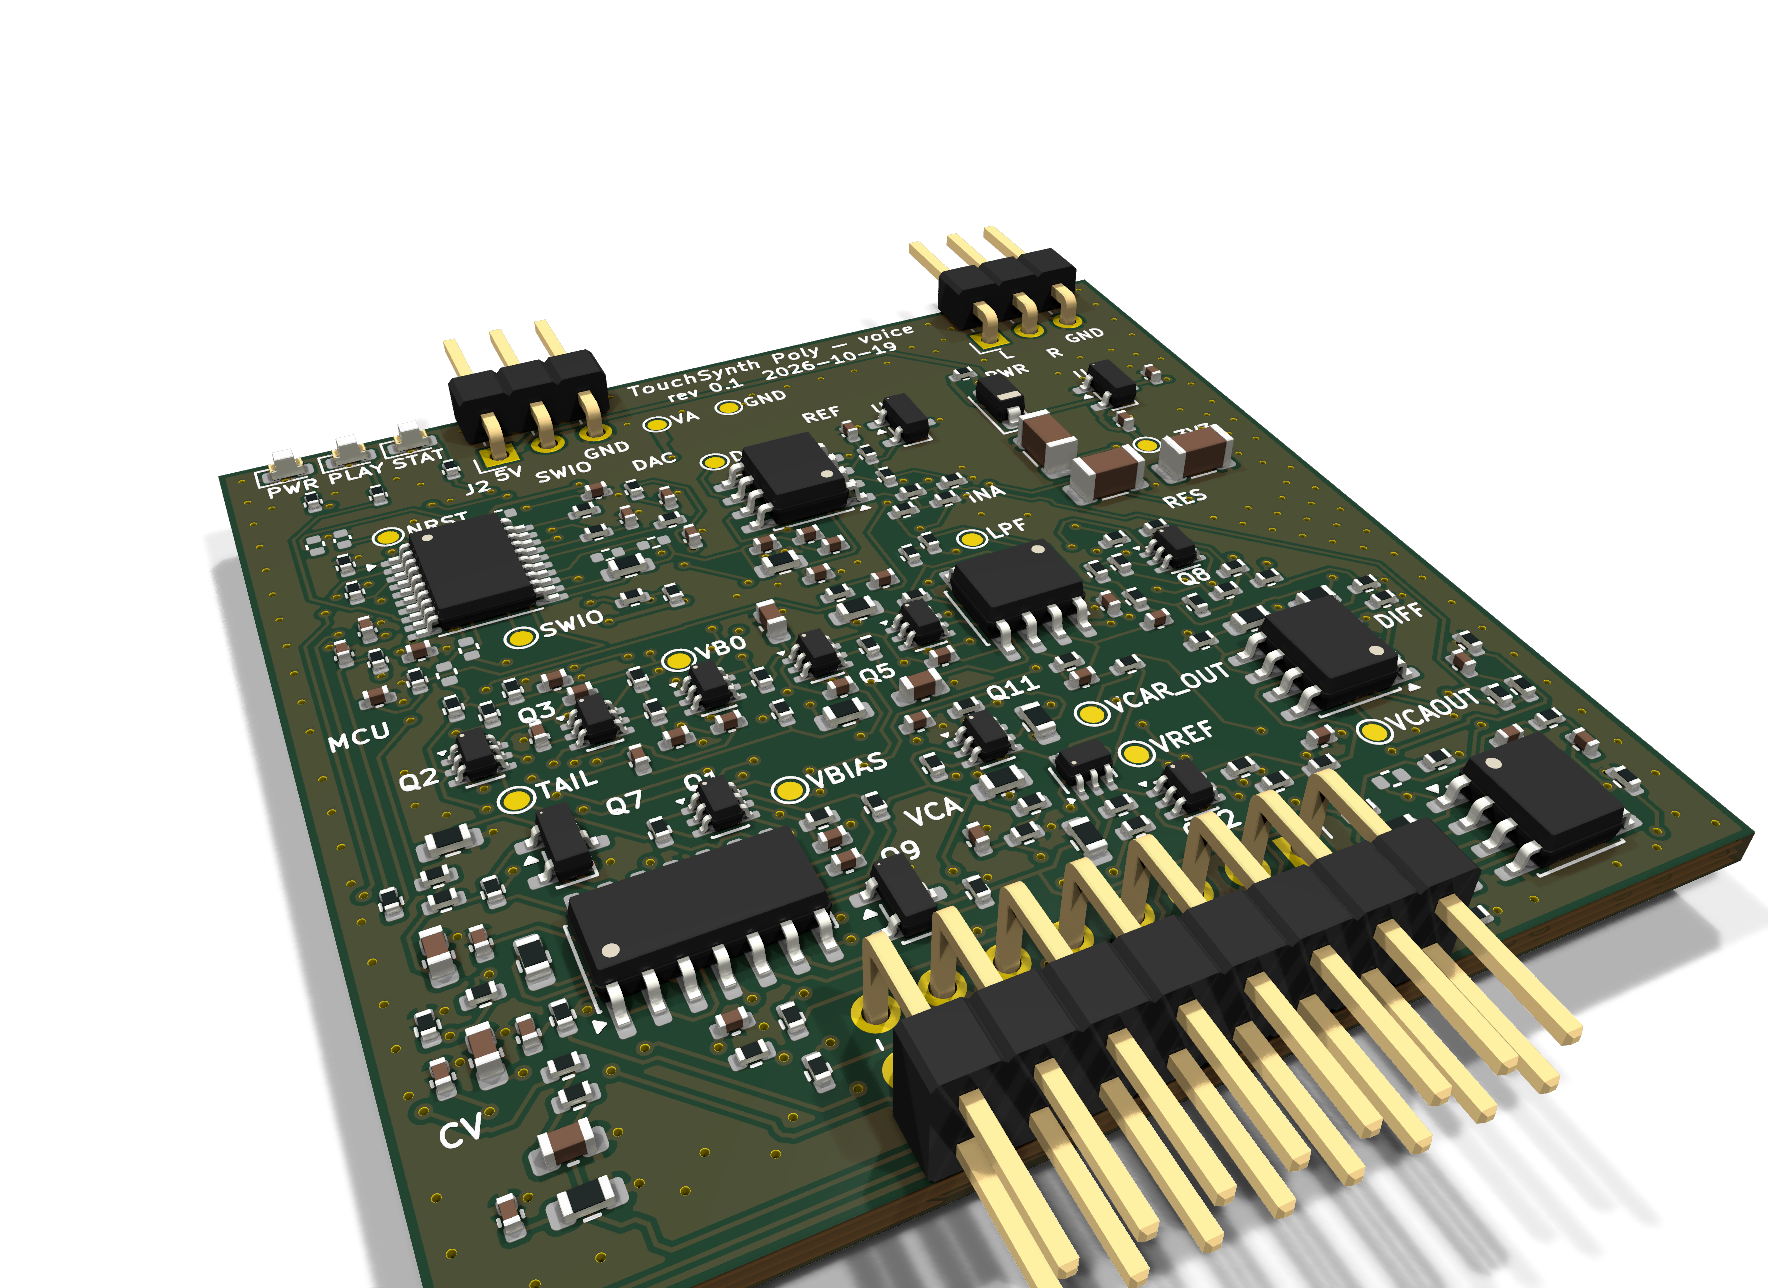
\includegraphics[width=\linewidth]{voice_pcb/render_iso.png}
    \caption{voice card, 50\,$\times$\,50\,mm, 4 layers}\end{subfigure}\hfill
  \begin{subfigure}{0.43\textwidth}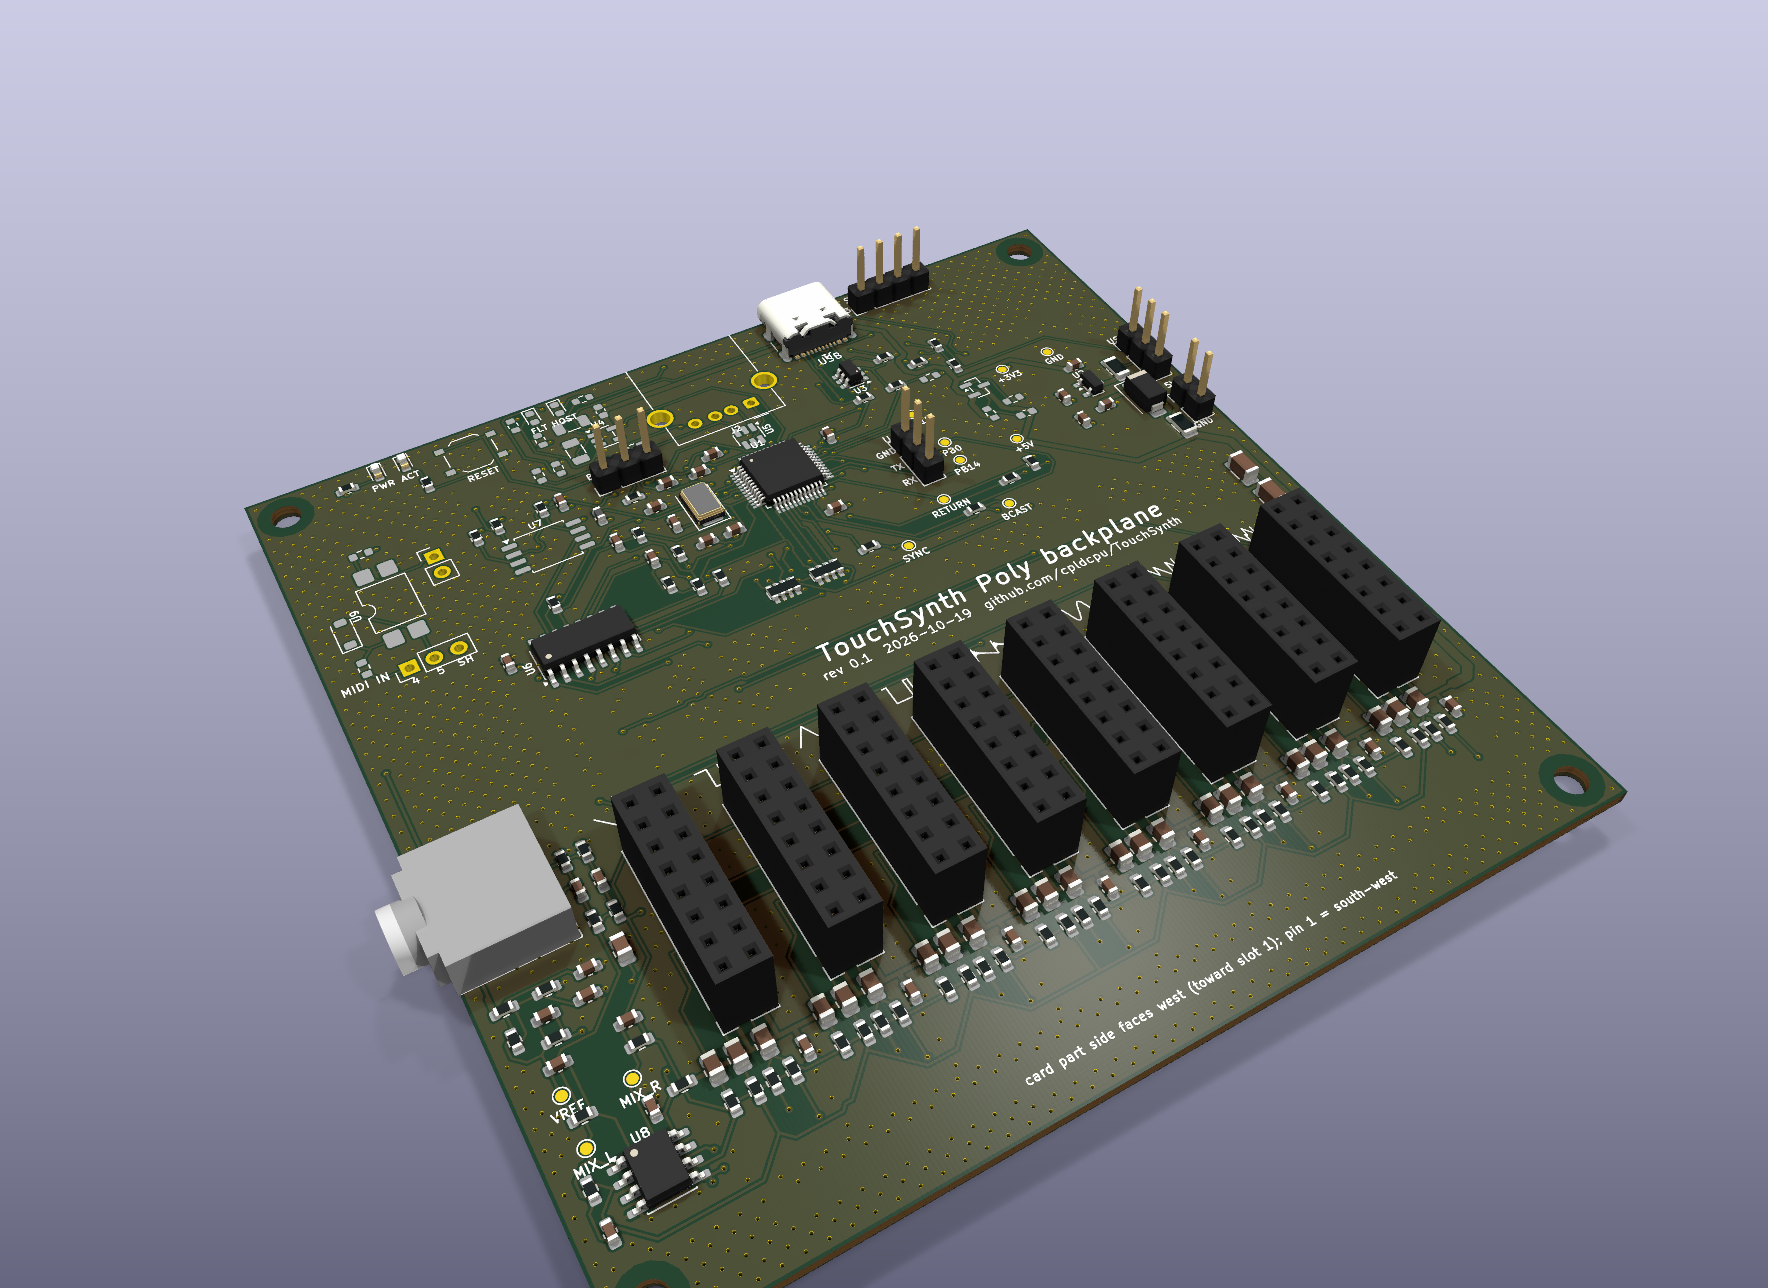
\includegraphics[width=\linewidth]{backplane_pcb/render_iso.png}
    \caption{backplane, 100\,$\times$\,100\,mm, 4 layers}\end{subfigure}
  \caption{KiCad 3D renders of the two boards, generated from the board files by \file{hw/pcb\_figures.py}.
  Not-fitted parts are left out.}
  \label{fig:hero}
\end{figure}

\clearpage
\tableofcontents
\clearpage

% =====================================================================================================================
\section{Overview}\label{sec:overview}

\subsection{What the instrument is}
TouchSynth Poly is a polyphonic analog synthesizer with 4 to 8 voices. It is played and edited from a computer
over USB, or from a class-compliant USB-MIDI keyboard. There are no controls on the instrument itself.
\begin{itemize}
  \item \textbf{Voice cards.} Each voice is an identical plug-in card of 50\,$\times$\,50\,mm. It carries:
    \begin{itemize}
      \item a CH32V006 that computes the oscillators and drives a PWM DAC and four PWM control voltages;
      \item the analog filter, resonance loop and VCA of TouchSynth rev 0.1, redesigned for \SI{5}{V};
      \item a stereo pan stage.
    \end{itemize}
    A card also runs on its own on the bench: it is powered and programmed by a WCH-LinkE and played from the
    SWIO console.
  \item \textbf{Backplane.} A board of 100\,$\times$\,100\,mm with eight slots. It carries:
    \begin{itemize}
      \item the CH32V203 controller with its crystal, the master clock of the instrument;
      \item USB-C (device: MIDI and CDC) and a USB-A host port for a keyboard (fitted; firmware in development);
      \item the voice bus;
      \item the power entry;
      \item the two-bus stereo mixer with the line output.
    \end{itemize}
\end{itemize}
The project is the successor of TouchSynth rev 0.1, a monophonic synthesizer with an analog DCO on one board, whose
report is on the \texttt{master} branch. The analog voice circuit and much of the firmware come from there; board~1 of
rev 0.1 served as the test bed for the oscillator engine, the DAC and the clock trimming.

\subsection{Constraints}
\begin{itemize}
  \item \textbf{Parts:} only JLCPCB \emph{Basic} and \emph{Promotional Extended} parts are assembled; the MCUs (own
    stock), connectors, headers and the few parts missing from the lists are hand-soldered.
  \item \textbf{MCUs:} CH32V006F8P7 (TSSOP-20, \SI{48}{MHz} from the internal HSI, \SI{8}{KB} RAM, \SI{62}{KB} flash)
    on the cards; CH32V203C8T6 (LQFP-48, \SI{144}{MHz} from an \SI{8}{MHz} crystal) on the backplane.
  \item \textbf{Supply:} a single \SI{5}{V} supply from USB-C or an external adapter, within \SI{500}{mA}.
  \item \textbf{Size:} voice cards at most 50\,$\times$\,50\,mm on 4 layers, at a slot pitch of \SI{10}{mm} (parts on one
    side, at most about \SI{6}{mm} high); backplane within 100\,$\times$\,100\,mm, planned as 2 layers, drawn and routed with 4.
  \item \textbf{Tools:} ch32fun, KiCad 10, ngspice. Schematics and boards are generated by Python scripts in
    \file{hw/} and checked against the simulation netlists.
\end{itemize}

\subsection{Requirements}
Tables~\ref{tab:reqf}--\ref{tab:reqp} summarise the requirements of \file{docs/design.md}. The status is
\emph{met} (measured on board~1 or simulated, as noted), \emph{design} (follows from the design, to be confirmed on
hardware) or \emph{open} (not yet shown).

\begin{table}[htbp]
\centering\small
\caption{Functional requirements (\file{docs/design.md} 2.1).}\label{tab:reqf}
\begin{tabularx}{\textwidth}{@{}l X >{\raggedright\arraybackslash}p{4.3cm}@{}}
\toprule
ID & Requirement & Status \\
\midrule
F1 & 4 to 8 voices on identical cards; any slot may be empty; the controller finds the populated slots at power-up
  & design (enumeration over per-slot NRST) \\
F2 & Played from a computer over USB-MIDI, class compliant & open \\
F3 & Played from a class-compliant USB-MIDI keyboard on a USB host port & open (port fitted; host driver in development, Section~\ref{sec:srsct}) \\
F4 & Configuration, presets and firmware updates over USB (CDC), cards included (SWIO from the controller)
  & open; SWIO programming through a V203 shown on the bench \\
F5 & Per voice: 3 oscillators, noise, modal drums; 4-pole ladder with resonance to self-oscillation; VCA; envelopes
  and modulation in firmware & met on board~1 (oscillators, drums, filter); on the bench card with the bus running,
  three oscillators take 23\,\% of the CPU (Section~\ref{sec:cpu}) \\
F6 & Multitimbral: up to 8 parts, each with channel, key range, voices, mode and patch & open (\file{midi.md}) \\
F7 & Stereo line out & design (pan on the card, S13) \\
F8 & Each card runs on its own (programmer power, SWIO console, own line out) & design \\
F9 & Each card calibrates itself through its audio loopback & met on board~1 (rev 0.1); to redo at \SI{5}{V} \\
F10 & Option: the mix as a USB audio input & open (ADC taps fitted) \\
F11 & Option: an effects card (reverb) in slot~1, mixing in or looping the whole mix through & design: backplane
  prepared
  (Section~\ref{sec:fxslot}) \\
\bottomrule
\end{tabularx}
\end{table}

\begin{table}[htbp]
\centering\small
\caption{Performance requirements (\file{docs/design.md} 2.2).}\label{tab:reqp}
\begin{tabularx}{\textwidth}{@{}l X l >{\raggedright\arraybackslash}p{5.0cm}@{}}
\toprule
ID & Requirement & Target & Status \\
\midrule
P1 & Pitch agreement between voices after start-up & $\leq$ 2\,cent & design: HSITRIM leaves $\leq \pm$1.8\,cent, then
  phase steps scaled to SYNC; HSI wander 0.35\,cent rms remains \\
P2 & Oscillator quality & as an analog DCO & met: equal to the DCO on board~1 (C2--C7) \\
P3 & DAC carrier at the line out & $\leq$ $-$70\,dB FS & met in simulation: \statSelevenCarrier\,dB (S11) \\
P4 & Signal-to-noise per voice & $\geq$ 65\,dB & met in simulation: \statStenSnrLo--\statStenSnrHi\,dB (S10) \\
P5 & Distortion at full drive, filter open & $\leq$ 1\,\% & met in simulation: \statStenThd\,\% (S10) \\
P6 & Cutoff range & 20\,Hz--20\,kHz & met in simulation: \statStenFcLow\,Hz--\statStenFcHigh\,kHz (S10) \\
P7 & Supply rejection 100\,Hz--10\,kHz & $\geq$ 60\,dB & met in simulation: 66--77\,dB (S10) \\
P8 & Latency, USB-MIDI note to sound & constant, $\leq$ 10\,ms & design: 6--7\,ms; bench: $D$ frames + 1--2 carrier
  periods \\
P9 & Power-up to playable, 8 cards & $\leq$ 3\,s & design: about 1\,s plus 0.3\,s per empty slot; bench: one card
  found 0.3--0.5\,s after a reset \\
P10 & Timing alignment between voices & $\leq$ 10\,\textmu s & design: a few \textmu s; bench (one card): latency
  spread 5--8\,\textmu s against SYNC, alignment between cards not yet measured \\
P11 & Long-term pitch drift between voices & none & design: locked to the controller's crystal \\
\bottomrule
\end{tabularx}
\end{table}

\subsection{System block diagram}
Figure~\ref{fig:system} shows the whole instrument. Table~\ref{tab:keyfig} lists its key figures; the numbers
marked as generated come from the design sources (\file{hw/voice.py}, \file{hw/backplane.py}) and the result files.

\begin{figure}[htbp]
\centering
\resizebox{\textwidth}{!}{%
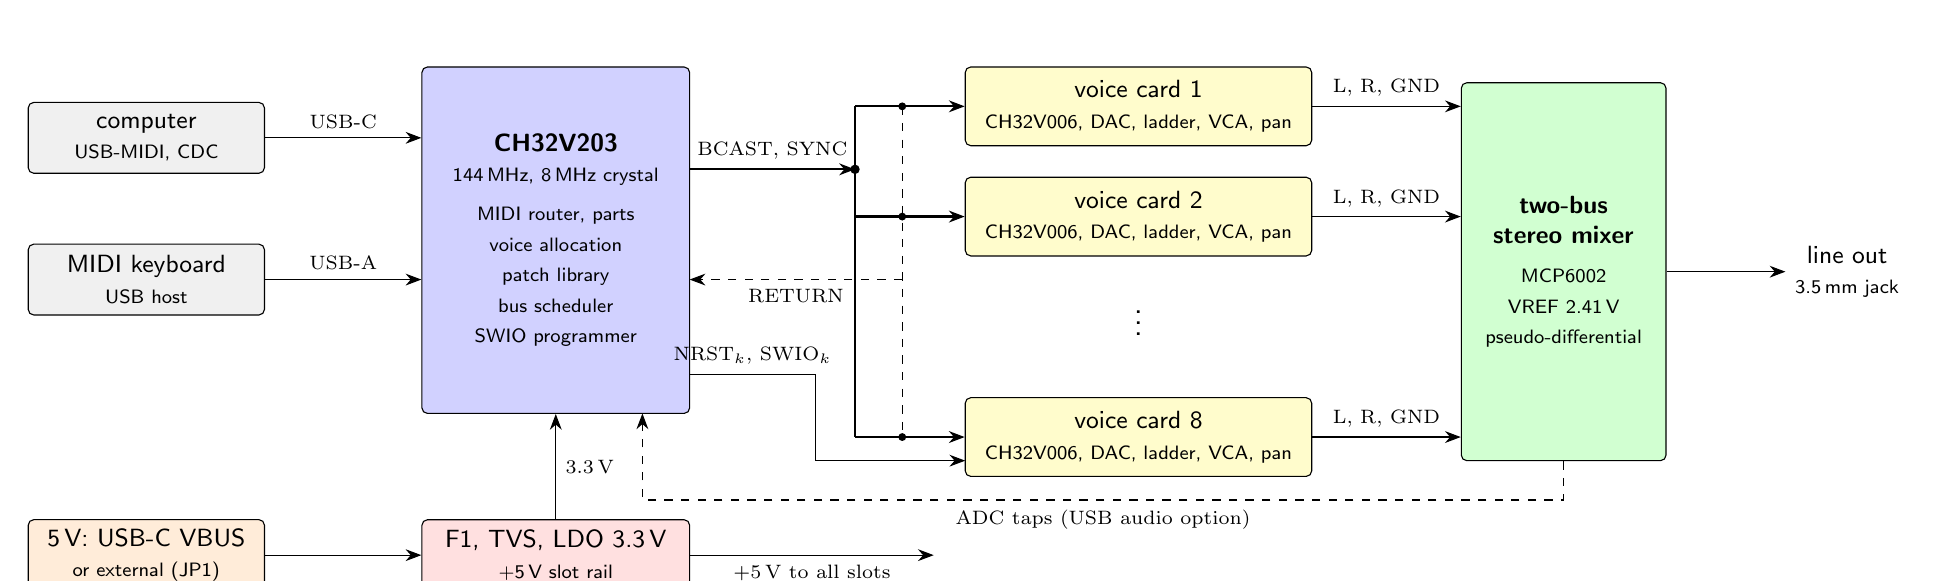
\begin{tikzpicture}[font=\small\sffamily, >={Stealth[length=2mm]},
  blk/.style={draw, rounded corners=2pt, fill=#1, minimum height=9mm, align=center}, blk/.default=white]
  \node[blk=gray!12, minimum width=30mm] (pc) at (0,2.4) {computer\\\scriptsize USB-MIDI, CDC};
  \node[blk=gray!12, minimum width=30mm] (kbd) at (0,0.6) {MIDI keyboard\\\scriptsize USB host};
  \node[blk=orange!15, minimum width=30mm] (pwr) at (0,-2.9) {5\,V: USB-C VBUS\\\scriptsize or external (JP1)};
  \node[blk=blue!18, minimum width=34mm, minimum height=44mm] (mcu) at (5.2,1.1)
    {\textbf{CH32V203}\\\scriptsize 144\,MHz, 8\,MHz crystal\\[3pt]\scriptsize MIDI router, parts\\\scriptsize voice
     allocation\\\scriptsize patch library\\\scriptsize bus scheduler\\\scriptsize SWIO programmer};
  \node[blk=red!12, minimum width=34mm] (ps) at (5.2,-2.9) {F1, TVS, LDO 3.3\,V\\\scriptsize +5\,V slot rail};
  \draw[->] (pc.east) -- node[above,font=\scriptsize]{USB-C} (pc.east -| mcu.west);
  \draw[->] (kbd.east) -- node[above,font=\scriptsize]{USB-A} (kbd.east -| mcu.west);
  \draw[->] (pwr) -- (ps);
  \draw[->] (ps.north) -- node[right,font=\scriptsize]{3.3\,V} (mcu.south);
  % cards
  \foreach \n/\y in {1/2.8, 2/1.4, 8/-1.4}
    \node[blk=yellow!20, minimum width=44mm, minimum height=10mm] (c\n) at (12.6,\y)
      {voice card \n\\\scriptsize CH32V006, DAC, ladder, VCA, pan};
  \node at (12.6,0.15) {\large$\vdots$};
  % broadcast and SYNC
  \draw[->, thick] (6.9,2.0) -- node[above,font=\scriptsize]{BCAST, SYNC} (9.0,2.0);
  \draw[thick] (9.0,2.8) -- (9.0,-1.4);
  \foreach \n in {1,2,8} \draw[->, thick] (c\n.west -| 9.0,0) -- (c\n.west);
  \fill (9.0,2.0) circle (0.6mm);
  % return
  \draw[dashed] (9.6,2.8) -- (9.6,-1.4);
  \foreach \n in {1,2,8} \fill (c\n.west -| 9.6,0) circle (0.5mm);
  \draw[->, dashed] (9.6,0.6) -- node[below,font=\scriptsize]{RETURN} (6.9,0.6);
  % NRST, SWIO
  \draw[->] (6.9,-0.6) -- node[above,font=\scriptsize]{NRST$_k$, SWIO$_k$} (8.5,-0.6) -- (8.5,-1.7) -- (10.4,-1.7);
  % mixer and out
  \node[blk=green!18, minimum width=26mm, minimum height=48mm] (mix) at (18.0,0.7)
    {\textbf{two-bus}\\\textbf{stereo mixer}\\[3pt]\scriptsize MCP6002\\\scriptsize VREF 2.41\,V\\\scriptsize
     pseudo-differential};
  \foreach \n in {1,2,8} \draw[->] (c\n.east) -- node[above,font=\scriptsize]{L, R, GND} (c\n.east -| mix.west);
  \node[align=center] (out) at (21.6,0.7) {line out\\\scriptsize 3.5\,mm jack};
  \draw[->] (mix) -- (out);
  \draw[->, dashed] (mix.south) -- (18.0,-2.2) -- node[below,font=\scriptsize]{ADC taps (USB audio option)}
    (6.3,-2.2) -- (6.3,-1.1);
  \draw[->] (ps.east) -- node[below,font=\scriptsize]{+5\,V to all slots} (10.0,-2.9);
\end{tikzpicture}}
\caption{System architecture. The controller is the only clock reference and the only bus master; the cards
receive one broadcast line and the SYNC frame clock and answer on a shared open-drain return line only when asked.
Each card returns its stereo signal and its own audio ground to the mixer.}
\label{fig:system}
\end{figure}

\begin{table}[htbp]
\centering\small
\caption{Key figures. \emph{gen.}: generated from the design sources or result files at build time.}\label{tab:keyfig}
\begin{tabularx}{\textwidth}{@{}>{\raggedright}p{7.4cm} >{\raggedright}X l@{}}
\toprule
Item & Value & Source \\
\midrule
Voices & 4--8 cards, 8 slots & design \\
Voice card: parts, nets, schematic sheets & \statVoiceParts, \statVoiceNets, \statVoiceSheets & gen. \\
Voice card: assembled parts, BOM lines, parts cost & \statVoiceAsm, \statVoiceLines, USD \statVoiceCost & gen. \\
Backplane: parts, nets, schematic sheets & \statBpParts, \statBpNets, \statBpSheets & gen. \\
Backplane: assembled parts, BOM lines, parts cost & \statBpAsm, \statBpLines, USD \statBpCost & gen. \\
Oscillators per voice & up to 3 (saw / pulse, polyBLEP), or modal drum & firmware \\
DAC & 7 bit, \SI{187.5}{kHz}, 2nd-order error feedback & firmware \\
Cutoff range (card, simulated) & \statStenFcLow\,Hz -- \statStenFcHigh\,kHz & gen.\ (S10) \\
Signal-to-noise, THD (card, simulated) & \statStenSnrLo--\statStenSnrHi\,dB, \statStenThd\,\% & gen.\ (S10) \\
DAC carrier at the line out (simulated) & \statSelevenCarrier\,dB re full scale & gen.\ (S11) \\
Stereo separation at hard pan, centre level (simulated) & \statSthirteenSep\,dB, \statSthirteenCentre\,dB per channel & gen.\ (S13) \\
Mixer: 8 cards hard-panned, in phase & \statStwelveHard\,V\sub{pp}, \statStwelveHardMargin\,dB below clipping & gen.\ (S12) \\
Voice bus & \SI{1}{Mbaud} 8N1, SYNC \SI{1}{kHz}, COBS, CRC-8 & bus.md \\
Latency MIDI $\to$ sound & 6--7\,ms, constant; alignment a few \textmu s & bus.md, bench \\
Supply & \SI{5}{V}, about 110--120\,mA for 8 cards & backplane.md \\
\bottomrule
\end{tabularx}
\end{table}

\subsection{Tool flow}
Every artefact is generated by scripts in the repository (Table~\ref{tab:tools}). For each board, one Python design
description is the single source of truth: schematic, PCB netlist and the simulation cross-check are derived from it.

\begin{table}[htbp]
\centering\small
\caption{Tool flow and where each step lives in the repository.}\label{tab:tools}
\begin{tabularx}{\textwidth}{@{}>{\raggedright}p{3.0cm} >{\raggedright}p{4.0cm} >{\raggedright\arraybackslash}X@{}}
\toprule
Step & Tool & Files \\
\midrule
Part selection & JLCPCB parts list (Basic + Promotional) & \file{parts/jlcpcb\_basic\_and\_promotional\_parts.csv}, \file{hw/lcsc.py} \\
Circuit simulation & ngspice-42 (WSL), Python & \file{sim/s10\_5v}, \file{s11\_recon}, \file{s12\_mixer}, \file{s13\_pan} \\
Behavioural model & Python + numba & \file{sim/behav/}, \file{sim/s9\_osc/} \\
Circuit description & Python & \file{hw/voice.py}, \file{hw/backplane.py} (\texttt{BOARD=backplane}) \\
Schematic & generated KiCad 10 schematic, hand-laid-out sheets & \file{hw/gen\_sch2.py}, \file{hw/layouts\_voice.py}, \file{hw/layouts\_backplane.py} \\
Checks & kicad-cli ERC, netlist and simulation cross-check & \file{hw/check\_netlist.py}, \file{hw/check\_sim.py} \\
PCB & KiCad 10 Python API, Freerouting, own maze router & \file{hw/gen\_pcb.py}, \file{hw/gen\_pcb\_bp.py}, \file{hw/pcb\_*.py} \\
Fabrication data, figures & kicad-cli & \file{hw/fab.py}, \file{hw/pcb\_figures.py} \\
Firmware & ch32fun, riscv64-unknown-elf-gcc (WSL) & \file{firmware/voice/}, \file{firmware/bench\_ctrl/} \\
Bench tests & Python, minichlink, oscilloscope over LAN & \file{tools/bustest.py}, \file{tools/buslib.py} \\
This report & Python, pdflatex & \file{docs/report/gen\_tables.py}, \file{touchsynth\_poly\_report.tex} \\
\bottomrule
\end{tabularx}
\end{table}

% =====================================================================================================================
\section{System architecture}\label{sec:arch}

\subsection{Partitioning}
Table~\ref{tab:part} gives the division of work between the controller and the cards.

\begin{table}[htbp]
\centering\small
\caption{Partitioning (\file{docs/design.md} 3.1).}\label{tab:part}
\begin{tabularx}{\textwidth}{@{}>{\raggedright}p{2.6cm} >{\raggedright}X >{\raggedright\arraybackslash}X@{}}
\toprule
Block & Responsibility & Why here \\
\midrule
Controller (backplane) & USB device and host, MIDI parsing, voice allocation, patch storage, bus master, clock
  reference, programming the cards & the only crystal; USB needs one; one place for the whole instrument's state \\
Voice card MCU & oscillators, envelopes, modulation, CV generation, self-calibration & \SI{48}{MHz} is enough for one
  voice, not for two; with the bus running, a three-oscillator voice takes 23\,\% (Section~\ref{sec:cpu}) \\
Voice card analog & reconstruction filter, expo converter, ladder, VCA, pan, loopback & the analog sound of rev 0.1;
  local references make the card independent of backplane ground \\
Mixer (backplane) & sum, line out, ADC feed & one stage for all cards, at the quiet end of the backplane \\
\bottomrule
\end{tabularx}
\end{table}

The main design choices and their basis:
\begin{itemize}
  \item \textbf{Digital oscillators on a PWM DAC instead of the analog DCO.} On board~1 the DAC saw and the DCO saw
    measure the same inharmonic content (S9, Section~\ref{sec:dac}). The DAC gives three oscillators, any waveform and
    the modal drums without extra parts.
  \item \textbf{\SI{187.5}{kHz} carrier, one sample per carrier period, second-order error feedback.} The sampling
    images, not the bit depth, limit the quality. At this rate 7 bits reach the quality of an ideal DAC in the model,
    and a \SI{31}{kHz} two-pole filter takes the carrier to \statSelevenCarrier\,dB (S11).
  \item \textbf{Single \SI{5}{V}.} Rail-to-rail MCP6002 op-amps replace the TL072s of rev 0.1. The core simulates
    within 1--2\,dB of rev 0.1 at less than half the current (S10).
  \item \textbf{UART broadcast with a SYNC line instead of SPI.} On the V006, SPI1 receive shares DMA channel~2 with
    the timer request that rev 0.1 used for the DAC; the UART receive ring runs on channel~5 beside the DAC and the CV
    burst (Section~\ref{sec:mcu}).
  \item \textbf{Synchronised HSI instead of a clock line.} Each card trims its oscillator to the SYNC pulses and scales
    its pitch to the measured frame period. A crystal-locked \SI{24}{MHz} clock line (CLK\_IN) remains as a fallback,
    fitted on demand.
  \item \textbf{Pan on the card, two mixing buses.} The card steers its VCA current into a left and a right output
    (S13); the backplane only sums (S12). Every slot is identical, and the stereo position is a firmware parameter.
\end{itemize}

\subsection{Clock and time base}\label{sec:clock}
There are two kinds of clock domain (Table~\ref{tab:clocks}).

\begin{table}[htbp]
\centering\small
\caption{Clock domains.}\label{tab:clocks}
\begin{tabularx}{\textwidth}{@{}l >{\raggedright}p{4.6cm} >{\raggedright\arraybackslash}X@{}}
\toprule
Domain & Source & Use \\
\midrule
Controller & \SI{8}{MHz} crystal, PLL $\times$18 = \SI{144}{MHz} & USB, bus baud rate, SYNC \SI{1}{kHz} (TIM1 CH1),
  \SI{24}{MHz} fallback clock (TIM3 CH4 = 144/6) \\
Each voice & own HSI, \SI{48}{MHz} after the fixed $\times$2 PLL, trimmed to SYNC & DAC carrier \SI{187.5}{kHz}, CV PWM
  \SI{46.875}{kHz}, UART divider, oscillator phase steps scaled by the measured SYNC period \\
\bottomrule
\end{tabularx}
\end{table}

\paragraph{SYNC.} The controller outputs a \SI{1}{kHz} square wave; its rising edge starts a \emph{frame}. Each card
takes its control tick (envelopes, LFOs, glide, CV laws, bus parsing) from this edge, so all cards compute on the same
ticks. Global LFOs take their phase from the frame number and stay phase-locked across voices without messages.

\paragraph{Clock trimming.} The HSI is specified at $\pm$\SI{2}{\percent}. A card first timestamps 100 SYNC periods
and sets HSITRIM; one trim step is about \SI{0.2}{\percent} (board~1: \SI{0.21}{\percent}, bench V006: $+0.19$ /
$-0.25$\,\%), so the residual is at most about $\pm$\SI{0.1}{\percent} or 1.8\,cent. Only then does it listen to the
bus: at \SI{1}{Mbaud} its USART divider is exactly 3.0 and cannot correct the clock itself. Afterwards the card keeps
measuring the SYNC period (filtered over about 64 frames) and scales its oscillators' phase steps by
48\,000\,/\,$\bar P$, so the pitch follows the crystal. What remains is the HSI's own short-term wander: board~1
showed flicker frequency noise with an Allan deviation of about $2\times10^{-4}$ from \SI{1}{ms} to \SI{0.5}{s}, i.e.
0.35\,cent rms, a slight independent wander of each voice similar to analog VCOs.

\paragraph{Presentation delay.} What a card computes in tick $n$ reaches its outputs at frame $n + D$, on every card:
CVs through a delay line, the oscillator state through a queue that the DAC renderer applies at the exact carrier
period. The controller stamps every event with its execution frame $L$ frames ahead. With $D = 4$ and $L = 2$ the
latency is 6--7\,ms and constant (details in Section~\ref{sec:bus}).

\subsection{Operating sequence}
\begin{enumerate}
  \item \textbf{Power-up:} the controller shifts zeros into the 74HC595, enables its outputs (all cards in reset)
    and starts SYNC and FRAME.
  \item \textbf{Enumeration:} slot by slot it releases NRST. The card measures SYNC, trims its HSI, starts its
    receiver and answers ASSIGN with HELLO (its 64-bit chip ID). A slot without HELLO within \SI{300}{ms} is empty.
    About \SI{1}{s} for 8 cards, plus \SI{0.3}{s} per empty slot.
  \item \textbf{Calibration} (on request): each card runs its loopback calibration; the controller keeps a copy of
    the results by chip ID.
  \item \textbf{Play:} MIDI events become timed voice messages on the broadcast line.
  \item \textbf{Update:} the controller reprograms a card over its SWIO line with an image received over CDC.
\end{enumerate}
A card that sees no SYNC within \SI{200}{ms} of reset runs standalone as a mono synth on its own HSI, controlled from
the SWIO console. This is also its state while the controller is in reset or in its bootloader: the 595 outputs are
then off, and the NRST lines float high through the cards' internal pull-ups.

\subsection{Power budget}\label{sec:power}
Table~\ref{tab:power} gives the current budget (\file{docs/backplane.md} 4.3).

\begin{table}[htbp]
\centering\small
\caption{Current budget at \SI{5}{V}.}\label{tab:power}
\begin{tabularx}{\textwidth}{@{}l r >{\raggedright\arraybackslash}X@{}}
\toprule
Load & Current & Basis \\
\midrule
8 voice cards & 80\,mA & about 10\,mA each: analog \statSthirteenCurrent\,mA (S13), MCU about 5\,mA, LEDs \\
CH32V203 at \SI{144}{MHz} & 12--20\,mA & datasheet: 11.8\,mA typical, plus USB and I/O \\
Mixer op-amps & \statStwelveSupply\,mA & S12 \\
LEDs & about 3\,mA & PWR, ACT (and HOST if fitted) \\
SWIO pull-up held low & 3.3\,mA & only while a card is being programmed \\
SPI flash (if fitted) & \textmu A standby & up to about 25\,mA while programming \\
\midrule
Synth & about 110--120\,mA & \\
Keyboard on USB-A & 50--200\,mA & limited at 0.5\,A by the TPS2051C \\
Total & at most about 425\,mA & inside a USB 2.0 port's 500\,mA \\
\bottomrule
\end{tabularx}
\end{table}

\paragraph{Inrush.} Each card filters its analog rail with \SI{22}{\ohm} and three \SI{100}{\micro F} X5R capacitors
(about \SI{35}{\micro F} each at \SI{5}{V}). Each card therefore limits its own inrush to about \SI{230}{mA},
decaying with $\tau \approx \SI{2.3}{ms}$; eight cards draw about \SI{1.8}{A} for a few milliseconds at plug-in. This
exceeds the USB attach allowance, but most ports tolerate it. The backplane keeps a P-channel soft-start switch as a
footprint, bridged by a \SI{0}{\ohm} resistor (Section~\ref{sec:bppower}). Before USB configuration the synth draws
about \SI{115}{mA} against the nominal \SI{100}{mA} limit; hosts rarely enforce it.

\paragraph{Supply margin.} The card works fully down to about \SI{4.3}{V} on its analog rail. Below that, full cutoff
combined with full resonance saturates the expo and resonance V$\to$I transistors; the audio path itself holds down
to \SI{4.0}{V}. With the \SI{22}{\ohm} rail filter (\SI{0.1}{V} drop) full function needs about \SI{4.4}{V} at the card
input, which a USB port's \SI{4.75}{V} minimum provides with typical cable loss.

\subsection{Card connector}
The card plugs into the backplane with a 2$\times$8 right-angle header on its bottom edge (Table~\ref{tab:conn}). All
logic is at \SI{3.3}{V} on both sides. Pin~6 carries the card's audio ground reference, joined on the card to the
ground pads of both output bleeders by its own track; the mixer uses it as the reference of its pseudo-differential
input.

\begin{table}[htbp]
\centering\small
\caption{Backplane connector, card side (J1 of \file{hw/voice.py}) and slot side (socket of \file{hw/backplane.py});
generated. Slot~1 differs on pins 3, 4, 14 and 15 (the effects slot, Section~\ref{sec:fxslot}).}\label{tab:conn}
% generated by gen_tables.py -- do not edit
\begin{tabular}{@{}r l l l@{}}
\toprule
Pin & Card net (J1) & Backplane net (slot $k$) & Function \\
\midrule
1 & \texttt{+5V} & \texttt{+5V} & supply \\
2 & \texttt{+5V} & \texttt{+5V} & supply \\
3 & \texttt{GND} & \texttt{GND} & ground \\
4 & \texttt{GND} & \texttt{GND} & ground \\
5 & \texttt{AUDIO\_\allowbreak{}L} & \texttt{AUDIO\_\allowbreak{}L\_\allowbreak{}k} & audio left (AC coupled, 100\,k$\Omega$ bleeder) \\
6 & \texttt{GND} & \texttt{AUDIO\_\allowbreak{}GND\_\allowbreak{}k} & audio ground reference (mixer mirror input) \\
7 & \texttt{AUDIO\_\allowbreak{}R} & \texttt{AUDIO\_\allowbreak{}R\_\allowbreak{}k} & audio right \\
8 & \texttt{GND} & \texttt{GND} & ground \\
9 & \texttt{SYNC} & \texttt{SYNC} & frame clock 1\,kHz \\
10 & \texttt{RX} & \texttt{BCAST} & broadcast in \\
11 & \texttt{TX} & \texttt{RETURN} & return (open drain) \\
12 & \texttt{NRST} & \texttt{NRST\_\allowbreak{}k} & reset / enumeration \\
13 & \texttt{GND} & \texttt{GND} & ground \\
14 & \texttt{SWIO} & \texttt{SWIO\_\allowbreak{}k} & programming \\
15 & \texttt{CLK\_\allowbreak{}IN} & \texttt{CLK} & 24\,MHz clock (option) \\
16 & \texttt{GND} & \texttt{GND} & ground \\
\bottomrule
\end{tabular}

\end{table}

% =====================================================================================================================
\section{Voice card}\label{sec:voice}

\subsection{Signal path}
Figure~\ref{fig:voicepath} shows the signal path. The firmware computes the oscillators at the carrier rate and writes
one 7-bit duty code per carrier period. A two-pole Sallen-Key filter removes the carrier, and the result drives the
ladder filter like rev 0.1's saw. Cutoff, resonance, VCA level, VCA trim and pan position are PWM outputs filtered by
RC networks. The schematic (\statVoiceSheets\ sheets) is reproduced in Appendix~\ref{app:sch}.

\begin{figure}[htbp]
\centering
\resizebox{\textwidth}{!}{%
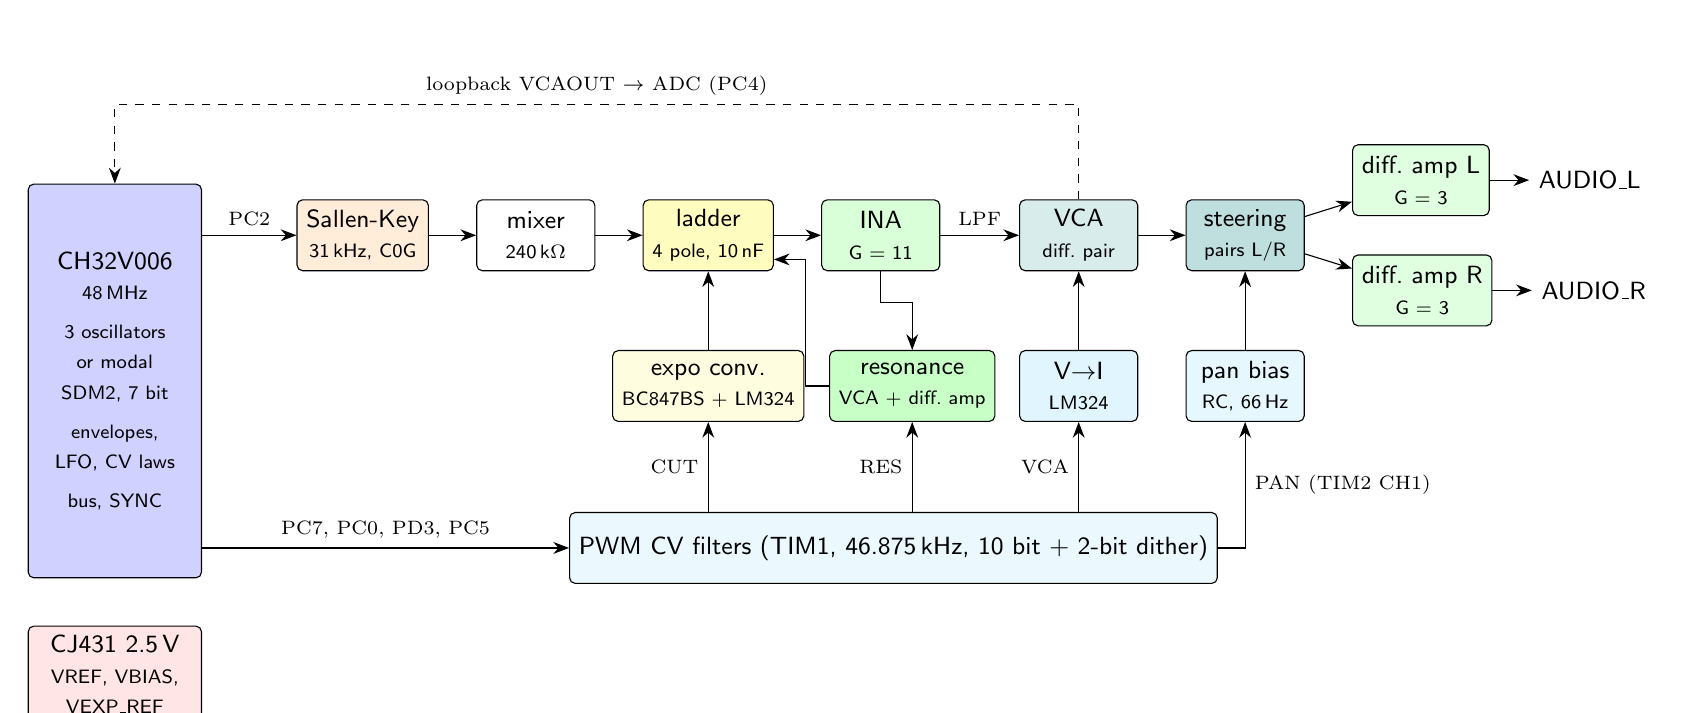
\begin{tikzpicture}[font=\small\sffamily, node distance=5mm and 6mm, >={Stealth[length=2mm]},
  blk/.style={draw, rounded corners=2pt, fill=#1, minimum height=9mm, minimum width=15mm, align=center},
  blk/.default=white]
  \node[blk=blue!18, minimum height=50mm, minimum width=22mm, align=center] (mcu) at (0,-1.6)
    {CH32V006\\\scriptsize 48\,MHz\\[3pt]\scriptsize 3 oscillators\\\scriptsize or modal\\\scriptsize SDM2, 7 bit\\[3pt]
     \scriptsize envelopes,\\\scriptsize LFO, CV laws\\[3pt]\scriptsize bus, SYNC};
  \node[blk=orange!15, right=12mm of mcu.north east, anchor=north west, yshift=-2mm] (sk) {Sallen-Key\\\scriptsize 31\,kHz, C0G};
  \node[blk=white, right=of sk] (mx) {mixer\\\scriptsize 240\,k$\Omega$};
  \node[blk=yellow!25, right=of mx] (lad) {ladder\\\scriptsize 4 pole, 10\,nF};
  \node[blk=green!15, right=of lad] (ina) {INA\\\scriptsize G = 11};
  \node[blk=teal!15, right=10mm of ina] (vca) {VCA\\\scriptsize diff.\ pair};
  \node[blk=teal!25, right=of vca] (pan) {steering\\\scriptsize pairs L/R};
  \node[blk=green!12, right=of pan, yshift=7mm] (dl) {diff.\ amp L\\\scriptsize G = 3};
  \node[blk=green!12, right=of pan, yshift=-7mm] (dr) {diff.\ amp R\\\scriptsize G = 3};
  \node[right=5mm of dl, align=left] (ol) {AUDIO\_L};
  \node[right=5mm of dr, align=left] (or) {AUDIO\_R};
  \draw[->] (sk) -- (mx); \draw[->] (mx) -- (lad); \draw[->] (lad) -- (ina); \draw[->] (ina) -- node[above,font=\scriptsize]{LPF} (vca);
  \draw[->] (vca) -- (pan); \draw[->] (pan) -- (dl); \draw[->] (pan) -- (dr); \draw[->] (dl) -- (ol); \draw[->] (dr) -- (or);
  \draw[->] (mcu.east |- sk) -- node[above,font=\scriptsize]{PC2} (sk);
  % lower row
  \node[blk=yellow!12, below=10mm of lad] (expo) {expo conv.\\\scriptsize BC847BS + LM324};
  \node[blk=green!22, below=10mm of ina, xshift=4mm] (res) {resonance\\\scriptsize VCA + diff.\ amp};
  \node[blk=cyan!12, below=10mm of vca] (vi) {V$\to$I\\\scriptsize LM324};
  \node[blk=cyan!10, below=10mm of pan] (pnet) {pan bias\\\scriptsize RC, 66\,Hz};
  \draw[->] (expo) -- (lad);
  \draw[->] (ina.south) -- ++(0,-4mm) -| (res.north);
  \draw[->] (res.west) -- ++(-3mm,0) |- ($(lad.south east)+(0,1.5mm)$);
  \draw[->] (vi) -- (vca); \draw[->] (pnet) -- (pan);
  % CV networks
  \node[blk=cyan!8, minimum width=80mm] (cvf) at ($(expo.south)!0.5!(vi.south)+(0,-16mm)$) {PWM CV filters (TIM1, 46.875\,kHz, 10 bit + 2-bit dither)};
  \draw[->] (cvf.north -| expo) -- node[left,font=\scriptsize]{CUT} (expo);
  \draw[->] (cvf.north -| res) -- node[left,font=\scriptsize]{RES} (res);
  \draw[->] (cvf.north -| vi) -- node[left,font=\scriptsize]{VCA} (vi);
  \draw[->] (cvf.east) -| node[pos=0.75,right,font=\scriptsize]{PAN (TIM2 CH1)} (pnet.south);
  \draw[->] (mcu.east |- cvf) -- node[above,font=\scriptsize]{PC7, PC0, PD3, PC5} (cvf.west);
  % loopback
  \draw[->, dashed] (vca.north) ++(0,0) -- ++(0,12mm) -| node[pos=0.25,above,font=\scriptsize]{loopback VCAOUT $\to$ ADC (PC4)} (mcu.north);
  % references
  \node[blk=red!10, below=6mm of mcu, minimum width=22mm] (ref) {CJ431 2.5\,V\\\scriptsize VREF, VBIAS,\\\scriptsize VEXP\_REF};
\end{tikzpicture}}
\caption{Voice card signal path. Dashed: the audio loopback used for calibration. Not drawn: the VCA trim (PC6, into
the VCA's second input) and the DAC low byte of the dual-PWM option.}
\label{fig:voicepath}
\end{figure}

\subsection{Digital oscillators and the PWM DAC (S9)}\label{sec:dac}
\paragraph{DAC.} TIM2 counts up and down over $2\times128$ ticks at \SI{48}{MHz}, a \SI{187.5}{kHz} carrier with
129 duty levels; the pulses are centred on the bottom of the count, so the signal does not modulate the pulse
position. The firmware computes one sample per carrier period and quantises it to 7 bits with second-order error
feedback (noise transfer function $(1-z^{-1})^2$).
\begin{itemize}
  \item \textbf{Loading (format 4):} in centre-aligned mode 2 a CH3 compare at 64 requests DMA1 channel~1 once per
    period, on the up-count only. The DMA writes the next code into the CH2 preload, which the update at the top of the
    count loads, so the pulse around the bottom stays symmetric. One byte per period: \SI{187500}{transfers/s}.
  \item \textbf{Start sequence:} TIM2 is reset through RCC and configured while stopped; the preloads are loaded with
    UG and the flags cleared; the DMA channel is armed and CC3DE set with the counter at 0; CEN comes last. On board~1,
    1000 starts in format~4 and 470 in format~3 showed no transfer before the first compare and exactly one entry at
    the first request; the read-back was exact over 2.0\,M and 0.96\,M requests.
  \item \textbf{Dual-PWM option:} TIM2 CH4 (PC1) drives a low byte into the filter input through
    \SI{1.33}{M\ohm} (\SI{1}{M\ohm} + \SI{330}{k\ohm}, not fitted) next to the high byte's \SI{11}{k\ohm}: 7 + 7 bits on
    the same carrier. A TIM2 DMA burst from the same request writes [high, 64, low] (format~3). The low-byte span is
    about 6\,\% larger than one high-byte step, so no tolerance leaves a gap; the firmware splits each sample with a
    ratio measured through the card's own loopback (null method, \file{docs/spec.md} 3.5).
\end{itemize}

\paragraph{Oscillators.} Up to three saw or pulse oscillators per voice (a pulse is the difference of two saws), each
with a two-point polyBLEP at the wrap; noise comes from an LFSR. A modal engine (resonator banks for drums, in fixed
point) renders \SI{15.625}{kHz} samples and interpolates them over 12 carrier periods. The rev 0.1 analog DCO, sub and
noise outputs are gone.

\paragraph{S9: DAC against DCO.} The behavioural model compared the analog DCO with several DAC variants on the same
filter, VCA and output (Table~\ref{tab:s9}, Figure~\ref{fig:s9}). The metric is the inharmonic content of a scale note
(aliasing and quantisation noise relative to the total, \SIrange{20}{20000}{Hz}). The rev 0.1 DAC mode (\SI{15.6}{kHz}
samples, interpolated) aliases at $-20$ to $-35$\,dB. One sample per carrier period at \SI{187.5}{kHz} with
second-order shaping comes within a few dB of the DCO. In the three-oscillator voice (Table~\ref{tab:s9moog}) the
\SI{93.75}{kHz} variants stay at $-22$ to $-38$\,dB whatever their resolution, because their sample-and-hold images
pass the filter; the \SI{187.5}{kHz} carrier reaches $-67$ to $-87$\,dB.

\begin{table}[htbp]
\centering\small
\caption{S9: inharmonic content [dB re total] of an open-filter saw in the behavioural model
(\file{docs/results/s9\_osc.csv}); generated. The card uses (h).}\label{tab:s9}
% generated by gen_tables.py -- do not edit
\begin{tabular}{@{}l l rrrr@{}}
\toprule
& Oscillator source & G2 & C4 & C6 & C7 \\
\midrule
(a) & analog DCO (rev 0.1) & $-$83.6 & $-$66.1 & $-$59.7 & $-$56.4 \\
(b) & DAC 15.6\,kHz samples, 8 bit, interpolated (rev 0.1) & $-$35.5 & $-$31.4 & $-$24.8 & $-$20.9 \\
(c) & 93.75\,kHz, 8 bit, one sample per period & $-$56.0 & $-$52.4 & $-$47.4 & $-$45.6 \\
(d) & as before + 2-pole filter & $-$58.7 & $-$55.0 & $-$49.8 & $-$47.7 \\
(e) & 93.75\,kHz dual PWM 16 bit + filter & $-$60.6 & $-$56.3 & $-$50.3 & $-$48.0 \\
(f) & 375\,kHz, 6 bit, SDM2, interpolated + filter & $-$62.1 & $-$58.3 & $-$53.7 & $-$53.3 \\
(g) & 187.5\,kHz, 7 bit, SDM2 & $-$69.4 & $-$63.0 & $-$59.2 & $-$58.3 \\
(h) & 187.5\,kHz, 7 bit, SDM2 + filter & $-$72.4 & $-$65.0 & $-$60.6 & $-$59.8 \\
\bottomrule
\end{tabular}

\end{table}

\begin{table}[htbp]
\centering\small
\caption{S9b: residual [dB] of a three-oscillator voice against an ideal DAC with the same filter
(\file{docs/results/s9\_moog.csv}); generated.}\label{tab:s9moog}
% generated by gen_tables.py -- do not edit
\begin{tabular}{@{}l r r r r@{}}
\toprule
Segment & 93.75\,kHz, SDM1 & 93.75\,kHz, SDM2 & 93.75\,kHz dual & 187.5\,kHz, SDM2 \\
\midrule
bass & $-$37.9 & $-$37.9 & $-$37.9 & $-$87.4 \\
lead & $-$22.4 & $-$22.4 & $-$22.4 & $-$66.7 \\
open & $-$26.8 & $-$26.8 & $-$26.8 & $-$69.5 \\
\bottomrule
\end{tabular}

\end{table}

\begin{figure}[p]
\centering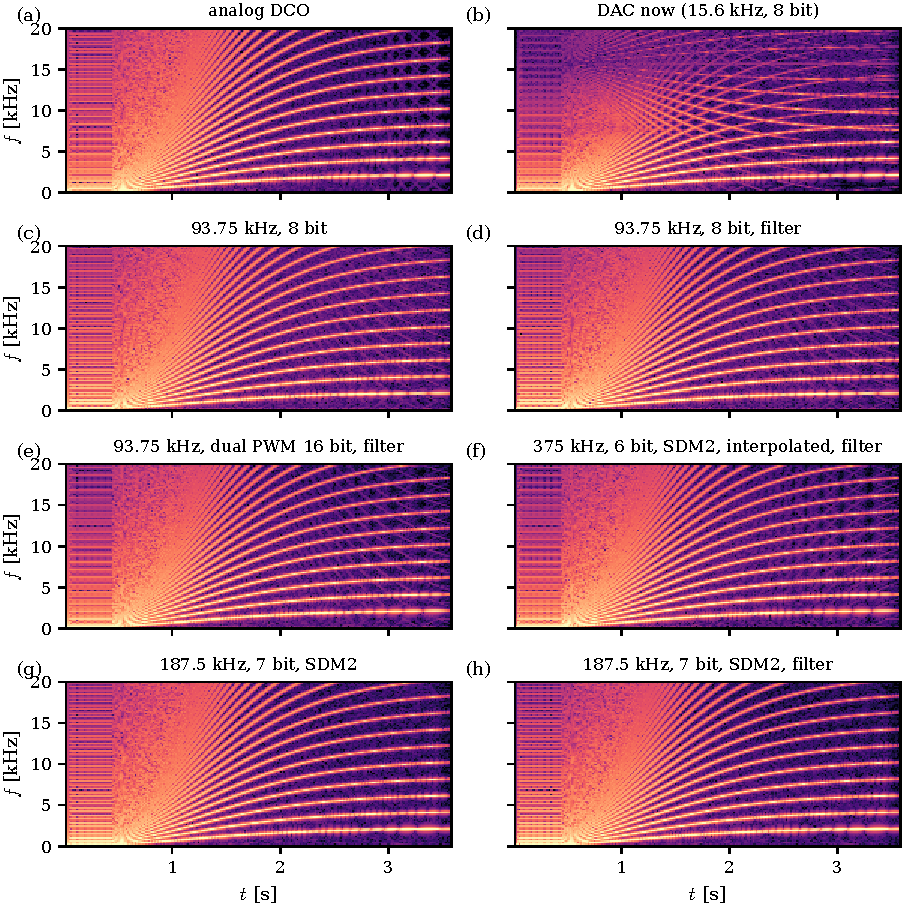
\includegraphics[width=0.92\textwidth]{s9_osc.pdf}
\caption{S9: spectrograms of the open-filter program (scale, glide C3$\to$C7) for the oscillator variants of
Table~\ref{tab:s9} in the behavioural model.}\label{fig:s9}
\end{figure}

\paragraph{Board~1.} The DAC was implemented on board~1 (rev 0.1 hardware, CH32V006), with the pulse output as the
DAC pin and the ladder as the only reconstruction filter. Saws from C2 to C7 through the open filter show the same
inharmonic content from the DCO and the DAC within about $\pm$2\,dB, and the same floor with the VCA closed
(Table~\ref{tab:hwdac}, Figure~\ref{fig:s9hw}). The DAC is about 3\,dB quieter there because board~1 feeds it through
\SI{470}{k\ohm}; the card uses \SI{240}{k\ohm} for the drive of rev 0.1's saw.

\begin{table}[htbp]
\centering\small
\caption{Board~1: saw C2--C7 from the analog DCO and from the PWM DAC, filter open
(\file{docs/results/hw\_board1\_dco\_vs\_dac.csv}); generated.}\label{tab:hwdac}
% generated by gen_tables.py -- do not edit
\begin{tabular}{@{}l r r r r r r@{}}
\toprule
& \multicolumn{3}{c}{analog DCO} & \multicolumn{3}{c}{PWM DAC} \\
\cmidrule(lr){2-4}\cmidrule(l){5-7}
Note & $f_0$ [Hz] & rms [mV] & inharm.\ [dB] & $f_0$ [Hz] & rms [mV] & inharm.\ [dB] \\
\midrule
C2 & 64.92 & 337 & $-$36.8 & 64.97 & 234 & $-$41.7 \\
C3 & 129.85 & 339 & $-$31.9 & 129.84 & 234 & $-$34.1 \\
C4 & 259.74 & 338 & $-$33.5 & 259.74 & 233 & $-$32.6 \\
C5 & 519.47 & 334 & $-$29.5 & 519.62 & 230 & $-$30.9 \\
C6 & 1039.06 & 325 & $-$32.0 & 1039.35 & 223 & $-$30.5 \\
C7 & 2079.16 & 309 & $-$36.1 & 2078.40 & 211 & $-$37.5 \\
\bottomrule
\end{tabular}

\end{table}

\begin{figure}[htbp]
\centering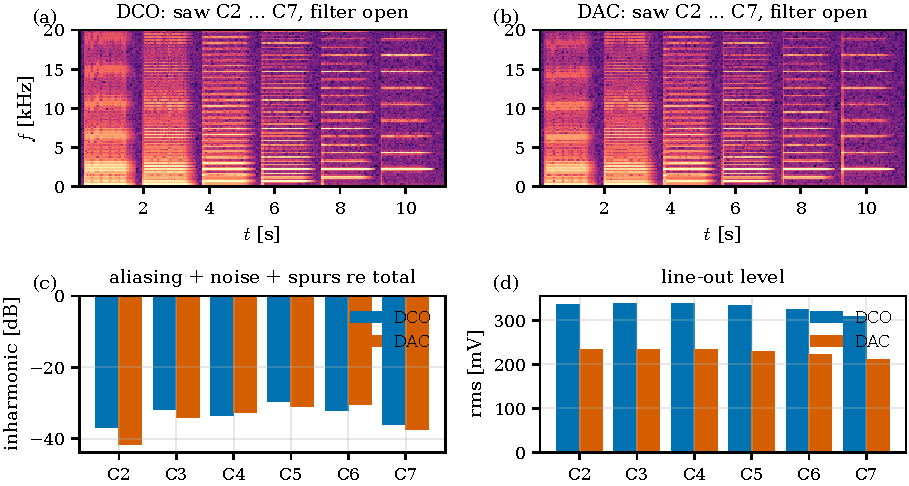
\includegraphics[width=0.92\textwidth]{s9_hwcmp.pdf}
\caption{Board~1: (a, b) spectrograms of the saw scale C2--C7 from the DCO and from the DAC; (c) inharmonic content;
(d) line-out level.}\label{fig:s9hw}
\end{figure}

\subsection{Reconstruction filter (S11)}
The DAC pin swings \SIrange{0}{3.3}{V}. A unity-gain Sallen-Key filter (one half of an MCP6002) removes the carrier
(Figure~\ref{fig:sk}):
\begin{itemize}
  \item \textbf{Values:} \SI{11}{k\ohm} / \SI{11}{k\ohm}, $C_1 = 2\times\SI{330}{pF}$ (feedback),
    $C_2 = \SI{330}{pF}$, all C0G. This is a Butterworth response at \SI{31}{kHz}; the simulated design used
    \SI{10}{k\ohm}, \SI{750}{pF}, \SI{375}{pF} (\SI{30}{kHz}). The C0G values on the JLCPCB lists near this range are
    \SI{100}{pF}, \SI{330}{pF} and \SI{2.2}{nF}, which set the values.
  \item \textbf{Result (S11):} the \SI{187.5}{kHz} carrier at \statSelevenCarrier\,dB re full scale at the line out,
    against \statSelevenCarrierNone\,dB without the filter; droop \statSelevenDroopTen\,dB at \SI{10}{kHz} and
    \statSelevenDroopTwenty\,dB at \SI{20}{kHz} (Table~\ref{tab:s11}).
  \item \textbf{Mixer resistor:} \SI{240}{k\ohm} (E24; S11 computed \statSelevenRmix\,k$\Omega$) gives the DAC's
    \SI{3.3}{V_{pp}} full scale the drive of rev 0.1's saw (\SI{2}{V_{pp}} through \SI{150}{k\ohm}).
  \item \textbf{Why not \SI{93.75}{kHz}:} that carrier would leave \statSelevenCarrierLow\,dB at the line out through
    the same filter. The dual-PWM option therefore runs on the \SI{187.5}{kHz} carrier as well.
  \item \textbf{Fixed cutoff:} the firmware shapes everything below Nyquist; the filter only removes carrier and
    images, so a voltage-controlled reconstruction filter is not needed.
\end{itemize}

\begin{figure}[htbp]
\centering
\begin{circuitikz}[scale=0.8, transform shape, font=\small]
  \draw (0,0) node[left]{PC2 (PWM\_DAC)} to[R, l=11\,k$\Omega$, o-*] (2.6,0) coordinate(sk1)
        to[R, l=11\,k$\Omega$, -*] (5.2,0) coordinate(sk2) -- (6.0,0) coordinate(pin);
  \draw (sk2) to[C, l_=330\,pF] (5.2,-2) node[ground]{};
  \draw (7.2,-0.5) node[op amp, noinv input up](OA){\scriptsize MCP6002};
  \draw (pin) |- (OA.+);
  \draw (OA.-) -- ++(-0.4,0) |- (8.8,-2.0) -- (8.8,-0.5);
  \draw (OA.out) -- (8.8,-0.5) node[circ]{} -- (9.6,-0.5) coordinate(daf);
  \draw (sk1) -- (2.6,1.6) to[C, l=2 $\times$ 330\,pF] (8.8,1.6) -- (8.8,-0.5);
  \draw (daf) node[above]{DAC\_F} to[R, l=240\,k$\Omega$, *-*] (12.2,-0.5) coordinate(mix) node[above]{MIX}
        to[C, l=1\,\textmu F, -o] (14.6,-0.5) node[right]{ladder BIN1};
  \draw (mix) to[R, l_=10\,k$\Omega$, -o] (12.2,-2.6) node[below]{VB0};
\end{circuitikz}
\caption{Reconstruction filter and mixer into the ladder input (all filter capacitors C0G). The dual-PWM low byte
joins at the first node through \SI{1.33}{M\ohm} (not fitted).}
\label{fig:sk}
\end{figure}

\begin{table}[htbp]
\centering\small
\caption{S11: carrier at the line out [dB re a full-scale tone] and in-band droop [dB] for reconstruction filter
variants on the \SI{5}{V} core (\file{docs/results/s11\_recon.csv}); generated.}\label{tab:s11}
% generated by gen_tables.py -- do not edit
\begin{tabular}{@{}l r r r r@{}}
\toprule
& \multicolumn{2}{c}{Carrier at the line out} & \multicolumn{2}{c}{Droop} \\
\cmidrule(lr){2-3}\cmidrule(l){4-5}
Filter & 93.75\,kHz & 187.5\,kHz & 10\,kHz & 20\,kHz \\
\midrule
none (DAC through $R_\mathrm{mix}$ only) & $-$18.3\,dB & $-$41.6\,dB & -- & -- \\
Sallen-Key 30\,kHz (as built: 31\,kHz) & $-$38.9\,dB & $-$74.1\,dB & $-$0.04 & $-$0.79 \\
Sallen-Key 25\,kHz & $-$42.0\,dB & $-$76.3\,dB & $-$0.09 & $-$1.54 \\
Sallen-Key 20\,kHz & $-$45.9\,dB & $-$78.1\,dB & $-$0.25 & $-$3.11 \\
Sallen-Key 15\,kHz & $-$50.7\,dB & $-$79.1\,dB & $-$0.79 & $-$6.35 \\
RC 25\,kHz + Sallen-Key 30\,kHz & $-$51.9\,dB & $-$92.0\,dB & $-$1.68 & $-$5.97 \\
RC 20\,kHz + Sallen-Key 25\,kHz & $-$56.4\,dB & $-$96.0\,dB & $-$2.46 & $-$8.05 \\
\bottomrule
\end{tabular}

\end{table}

\subsection{The \SI{5}{V} ladder core (S10)}
The analog core of rev 0.1 ran from \SIrange{8.6}{11.6}{V} with TL072s and a \SI{4.5}{V} reference. S10 redesigned it
for \SI{5}{V} in steps (variants v5, v5r, v5m) and checked the card as built (v5c). The changes:
\begin{itemize}
  \item \textbf{Op-amps:} MCP6002 (rail-to-rail) for the VREF buffer, the instrumentation amplifier, the difference
    amplifiers and the reconstruction filter (four packages including the pan stage); the LM324 keeps the three
    V$\to$I converters and buffers VBIAS.
  \item \textbf{References:} VREF = \SI{2.5}{V} from a CJ431 (fed by \SI{1}{k\ohm} from the analog rail, then
    \SI{10}{k\ohm} / \SI{10}{\micro F}, buffered); VEXP\_REF = \SI{1.25}{V} (VREF/2) at the expo reference transistor's
    collector; VBIAS = \SI{1.0}{V}, buffered by the LM324's fourth unit. The buffer is needed: the expo divider's CV
    current would move a bare divider by up to \SI{0.6}{V}.
  \item \textbf{CV range:} the MCU runs at \SI{3.3}{V}, so the PWM CVs span \SIrange{0}{3.3}{V}. The expo divider is
    \SI{18}{k\ohm} / \SI{1.5}{k\ohm} to VBIAS; the linear networks end in \SI{12}{k\ohm} (resonance) and \SI{3}{k\ohm}
    (VCA).
  \item \textbf{Ladder:} four poles with \SI{10}{nF} (rev 0.1: \SI{33}{nF}) and \SI{470}{k\ohm} from VREF for the expo
    reference current, so the same cutoffs are reached at a third of the tail current and the expo op-amp keeps room
    at the top. Bias chain \SI{620}{\ohm} / 4$\times$\SI{1.5}{k\ohm} / \SI{3.3}{k\ohm} from the analog rail: VB0 =
    \SI{1.66}{V}, stage spacing \SI{0.76}{V}, so the rungs keep about \SI{0.1}{V} of reverse $V_\mathrm{CB}$ (at
    \SI{0.6}{V} spacing they touch saturation and distort).
  \item \textbf{Instrumentation amplifier:} two MCP6002 units, gain 11, output referenced to VREF. Its inputs sit at
    \SIrange{4.04}{4.24}{V} over the whole cutoff range, above the MCP6002's input-stage transition (typically near
    $V_\mathrm{DD} - \SI{1.1}{V}$).
  \item \textbf{Analog rail:} VA behind \SI{22}{\ohm} and $3\times\SI{100}{\micro F}$ X5R 1206 (no \SI{220}{\micro F}
    part on the lists; about \SI{35}{\micro F} each at \SI{5}{V}).
\end{itemize}
Table~\ref{tab:s10} compares rev 0.1 with the \SI{5}{V} core and the card as built; Figure~\ref{fig:s10} shows the
cutoff law and the distortion. The card covers \statStenFcLow\,Hz to \statStenFcHigh\,kHz, self-oscillates from the
same resonance CV as rev 0.1, and stays within about 1--2\,dB of it, at \statStenCurrent\,mA analog current instead of
\SI{9.1}{mA}. The vendor MCP6002 macromodel used for v5m and v5c (Microchip MCP6001/2/4, REV G) is licensed for use
with Microchip parts and is not in the repository; it has one NMOS input pair and therefore no input crossover and no
distortion detail.

\begin{table}[htbp]
\centering\small
\caption{S10: the analog core at \SI{5}{V} against rev 0.1 (\file{docs/results/s10\_5v.csv}); generated. CV values
are fractions of the PWM full scale expressed on a \SI{5}{V} scale; drive levels are saw equivalents
(\SI{2}{V_{pp}} = full DAC scale).}\label{tab:s10}
\setlength{\tabcolsep}{4pt}
% generated by gen_tables.py -- do not edit
\begin{tabular}{@{}l rrrr@{}}
\toprule
Quantity & \shortstack[r]{v12\\[-1pt]\footnotesize rev 0.1, 8.6\,V} & \shortstack[r]{v5m\\[-1pt]\footnotesize 5\,V, MCP6002 model} & \shortstack[r]{v5c\\[-1pt]\footnotesize card as built} & \shortstack[r]{v5c46\\[-1pt]\footnotesize card at 4.6\,V} \\
\midrule
$-3$\,dB cutoff, CV\sub{CUT} = 0 & 20.1\,Hz & 18.9\,Hz & 18.8\,Hz & 18.8\,Hz \\
$-3$\,dB cutoff, CV\sub{CUT} = full scale & 20.2\,kHz & 30.6\,kHz & 30.4\,kHz & 30.4\,kHz \\
resonance peak, CV\sub{RES} = 2.5 (5\,V scale) & 19.6\,dB & 22.6\,dB & 22.7\,dB & 22.8\,dB \\
self-oscillation threshold (5\,V scale) & 3.1 & 3.0 & 3.0 & 3.0 \\
THD at 2\,V\sub{pp} saw-equivalent drive & 0.58\,\% & 0.44\,\% & 0.47\,\% & 0.47\,\% \\
line out at that drive & 1.20\,V\sub{pp} & 1.37\,V\sub{pp} & 1.46\,V\sub{pp} & 1.46\,V\sub{pp} \\
signal-to-noise, filter open & 69.8\,dB & 68.2\,dB & 68.8\,dB & 68.8\,dB \\
supply rejection, 100\,Hz & $-$80\,dB & $-$61\,dB & $-$69\,dB & $-$69\,dB \\
\quad 1\,kHz & $-$84\,dB & $-$65\,dB & $-$66\,dB & $-$66\,dB \\
\quad 10\,kHz & $-$71\,dB & $-$78\,dB & $-$77\,dB & $-$77\,dB \\
smallest $V_\mathrm{CE}$ over the CV corners & 0.73\,V & 0.51\,V & 0.50\,V & 0.37\,V \\
analog supply current & 9.1\,mA & 3.6\,mA & 4.0\,mA & 3.9\,mA \\
\bottomrule
\end{tabular}

\end{table}

\begin{figure}[htbp]
\centering
\resizebox{\textwidth}{!}{% generated by gen_tables.py -- do not edit
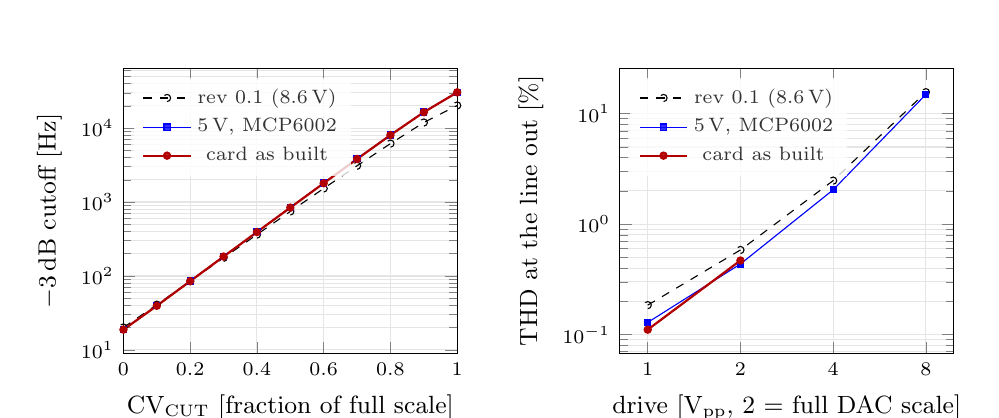
\begin{tikzpicture}
\begin{semilogyaxis}[width=0.48\textwidth,height=5.2cm,xlabel={CV\sub{CUT} [fraction of full scale]},ylabel={$-3$\,dB cutoff [Hz]},xmin=0,xmax=1,grid=both,grid style={black!10},legend pos=north west,legend style={font=\scriptsize,draw=none,fill=white,fill opacity=0.8},tick label style={font=\scriptsize},label style={font=\small}]
\addplot[black,dashed,mark=o,mark size=1.3pt] coordinates {(0.00,20.1) (0.10,40.9) (0.20,84.9) (0.30,175.9) (0.40,363.0) (0.50,746.2) (0.60,1526.9) (0.70,3095.1) (0.80,6165.3) (0.90,11899.0) (1.00,20224.2)}; \addlegendentry{rev 0.1 (8.6\,V)}
\addplot[blue,mark=square*,mark size=1.1pt] coordinates {(0.00,18.9) (0.10,39.7) (0.20,85.5) (0.30,184.0) (0.40,394.8) (0.50,845.6) (0.60,1807.7) (0.70,3844.7) (0.80,8083.7) (0.90,16497.1) (1.00,30572.8)}; \addlegendentry{5\,V, MCP6002}
\addplot[red!70!black,thick,mark=*,mark size=1.1pt] coordinates {(0.00,18.8) (0.10,39.5) (0.20,85.1) (0.30,183.0) (0.40,392.5) (0.50,840.9) (0.60,1797.2) (0.70,3823.5) (0.80,8039.5) (0.90,16407.3) (1.00,30449.1)}; \addlegendentry{card as built}
\end{semilogyaxis}
\begin{semilogyaxis}[xshift=0.52\textwidth,width=0.48\textwidth,height=5.2cm,xlabel={drive [V\sub{pp}, 2 = full DAC scale]},ylabel={THD at the line out [\%]},xmode=log,log basis x=2,xtick={1,2,4,8},xticklabels={1,2,4,8},grid=both,grid style={black!10},legend pos=north west,legend style={font=\scriptsize,draw=none,fill=white,fill opacity=0.8},tick label style={font=\scriptsize},label style={font=\small}]
\addplot[black,dashed,mark=o,mark size=1.3pt] coordinates {(1,0.185) (2,0.584) (4,2.478) (8,15.651)}; \addlegendentry{rev 0.1 (8.6\,V)}
\addplot[blue,mark=square*,mark size=1.1pt] coordinates {(1,0.129) (2,0.436) (4,2.046) (8,14.934)}; \addlegendentry{5\,V, MCP6002}
\addplot[red!70!black,thick,mark=*,mark size=1.1pt] coordinates {(1,0.111) (2,0.469)}; \addlegendentry{card as built}
\end{semilogyaxis}
\end{tikzpicture}
}
\caption{S10: (left) $-3$\,dB cutoff versus CV\sub{CUT}; (right) THD at the line out versus drive, filter open
(generated from \file{docs/results/s10\_5v.csv}).}\label{fig:s10}
\end{figure}

\subsection{Resonance}
The resonance loop is a voltage-controlled amplifier of its own, as in rev 0.1:
\begin{itemize}
  \item the filter output (LPF) is AC coupled through \SI{1}{\micro F} and \SI{120}{k\ohm} into a BC847BS differential
    pair biased from VB2;
  \item its tail current comes from CV\sub{RES} through an LM324 V$\to$I converter (\SI{12}{k\ohm} last network stage,
    $R_E$ = \SI{3.6}{k\ohm});
  \item the collectors (\SI{4.7}{k\ohm}) feed an MCP6002 unity difference amplifier, whose output returns through
    \SI{4.7}{\micro F} and \SI{22}{k\ohm} into the ladder's second input. The difference amplifier removes the
    common-mode step of the collectors when the tail current changes. Its inputs sit at
    \SIrange{3.2}{3.75}{V}, below the MCP6002 input transition.
\end{itemize}

\subsection{VCA and trim}
\begin{itemize}
  \item \textbf{Core:} a BC847BS pair, input attenuated by \SI{33}{k\ohm} into \SI{1}{k\ohm} to VCA\_BIAS = \SI{1.89}{V}
    (\SI{2.4}{k\ohm} / \SI{7.5}{k\ohm} from VREF). The low base bias leaves room for the steering pairs stacked on
    the collectors.
  \item \textbf{Tail:} an LM324 V$\to$I converter ($R_E$ = \SI{1.2}{k\ohm}, \SI{0.6}{mA} full scale, as before). A
    \SI{240}{k\ohm} resistor from VREF to the emitter makes the current truly zero at CV = 0 despite the op-amp
    offset.
  \item \textbf{Trim:} rev 0.1 trimmed the CV feed-through with an 8-bit R-2R DAC on a 74HC595. The card uses the
    former CV\sub{AMP} PWM channel (TIM1 CH1, PC6) through $2\times$(\SI{10}{k\ohm}, \SI{1}{\micro F}) and
    \SI{680}{k\ohm} into the second base, with \SI{5.1}{M\ohm} from the first base to ground: about
    $\pm$\SI{2.4}{mV} at the pair input around mid scale. S13 found the nulling trim at about \SI{0.92}{V} and a
    residual of \SI{0.03}{mV} for the mono VCA.
  \item \textbf{Difference amplifiers:} the VCA difference amplifiers have matched \SI{33}{k\ohm} from both inputs to
    ground. This keeps their inputs at \SIrange{2.44}{3.13}{V}, below the MCP6002 input transition, which they would
    otherwise cross during every attack (an offset step of about \SI{1.6}{mV} at the output).
  \item \textbf{Loopback:} \SI{10}{k\ohm} / \SI{15}{k\ohm} with \SI{1}{nF} from VCAOUT (left channel) to PC4 (ADC A2)
    for the calibration.
\end{itemize}

\subsection{Stereo pan stage (S13)}\label{sec:pan}
S13 compared two ways to give each card a stereo output (Table~\ref{tab:s13}):
\begin{itemize}
  \item \textbf{A, current steering (built):} two more BC847BS pairs sit on the VCA collectors (Figure~\ref{fig:pan}).
    The L transistors' bases are at VREF, the R transistors' bases at PAN\_B = VREF $-143 \ldots +149$\,mV, set by
    the PC5 PWM (TIM2 CH1) through \SI{27}{k\ohm}, with \SI{24}{k\ohm} to +3V3, \SI{3}{k\ohm} to VREF and
    \SI{1}{\micro F} (\SI{66}{Hz}, centre at 49\,\% duty). The left output receives $\alpha\,\Delta I$, the right
    $(1-\alpha)\,\Delta I$: a linear law.
  \item \textbf{B, a second VCA:} a complete second pair with its own CV.
\end{itemize}
A was chosen: one envelope CV (the fine 10 + 2-bit channel), calibration from the existing loopback and fewer parts.
Its costs:
\begin{itemize}
  \item the VCA is re-biased (bases at \SI{1.89}{V});
  \item a fourth MCP6002 is needed (the R difference amplifier; its other unit is a spare follower);
  \item the linear pan law is corrected in firmware: CV\sub{VCA} is raised towards the centre for constant power and
    capped at 70.6\,\% at hard pan;
  \item a steering-pair mismatch gives a click at the centre, about \statSthirteenClick\,mV per mV of mismatch (opposite
    in L and R), and none at hard pan.
\end{itemize}
Both difference amplifiers run at a gain of 3.0 (\SI{10}{k\ohm} / \SI{30}{k\ohm}) and drive the outputs through
\SI{100}{\ohm} and \SI{10}{\micro F} with a \SI{100}{k\ohm} bleeder. Simulated at \SI{5}{V}: centre
\statSthirteenCentre\,dB per channel, separation \statSthirteenSep\,dB, THD \statSthirteenThd\,\%, SNR
\statSthirteenSnr\,dB, \statSthirteenCurrent\,mA analog current, \statSthirteenParts\ parts added.

\begin{figure}[htbp]
\centering
\begin{circuitikz}[scale=0.64, transform shape, font=\small]
  % VCA pair
  \draw (0,0) node[npn](QA1){} (8.1,0) node[npn, xscale=-1](QA2){};
  \draw (QA1.E) -- ++(0,-0.5) coordinate(e1) -- (e1 -| QA2.E) coordinate(e2) -- (QA2.E);
  \draw ($(e1)!0.5!(e2)$) node[circ]{} to[I, l_=$I_\mathrm{tail}$ (CV\sub{VCA})] ++(0,-2.0) node[ground]{};
  \draw (QA1.B) -- ++(-0.6,0) node[left]{\shortstack[r]{VCA\_IN1\\(audio, 1.89\,V)}};
  \draw (QA2.B) -- ++(0.6,0) node[right]{\shortstack[l]{VCA\_IN2\\(trim)}};
  % steering pairs on each collector
  \draw (QA1.C) -- ++(0,0.4) coordinate(c1);
  \draw (-1.4,2.1) node[npn](SL1){} (1.4,2.1) node[npn, xscale=-1](SR1){};
  \draw (SL1.E) |- (c1); \draw (SR1.E) |- (c1);
  \draw (QA2.C) -- ++(0,0.4) coordinate(c2);
  \draw (6.7,2.1) node[npn](SL2){} (9.5,2.1) node[npn, xscale=-1](SR2){};
  \draw (SL2.E) |- (c2); \draw (SR2.E) |- (c2);
  \draw (SL1.B) -- ++(-0.3,0) node[left]{VREF};
  \draw (SR1.B) -- ++(0.3,0) node[right]{PAN\_B};
  \draw (SL2.B) -- ++(-0.3,0) node[left]{VREF};
  \draw (SR2.B) -- ++(0.3,0) node[right]{PAN\_B};
  \foreach \t/\l in {SL1/L1, SR1/R1, SL2/L2, SR2/R2}
    \draw (\t.C) -- ++(0,0.4) node[above]{\l};
  \node[draw, rounded corners=2pt, align=left, font=\scriptsize, anchor=west] at (12.0,1.0)
    {L1, L2, R1, R2: 4.7\,k$\Omega$ to VA\\
     L1 $-$ L2 $\to$ difference amp L (G = 3) $\to$ AUDIO\_L\\
     R1 $-$ R2 $\to$ difference amp R (G = 3) $\to$ AUDIO\_R\\[2pt]
     PAN\_B = VREF $-$143 \ldots\ +149\,mV:\\
     PC5 PWM $\to$ 27\,k$\Omega$, 24\,k$\Omega$ to +3V3,\\
     3\,k$\Omega$ to VREF, 1\,\textmu F};
\end{circuitikz}
\caption{Stereo pan stage (S13 variant A, simplified): two steering pairs on the VCA collectors divide each collector
current between the left and the right load resistors.}
\label{fig:pan}
\end{figure}

\begin{table}[htbp]
\centering\small
\caption{S13: pan stage variants at \SI{5}{V}, one card (\file{docs/results/s13\_pan.csv}); generated. The click is the
step at the line out when the VCA opens, per \SI{1}{mV} of steering-pair mismatch (A) or for an untrimmed second VCA
(B).}\label{tab:s13}
% generated by gen_tables.py -- do not edit
\begin{tabular}{@{}l r r@{}}
\toprule
Quantity & A: current steering (built) & B: second VCA \\
\midrule
Parts added to the card & 22 & 26 \\
Area (courtyards) & 135\,mm\textsuperscript{2} (5.4\,\%) & 159\,mm\textsuperscript{2} (6.4\,\%) \\
Centre: level per channel & $-$3.5\,dB & $-$3.2\,dB \\
Centre: total power & $-$0.45\,dB & $-$0.22\,dB \\
Channel separation, hard pan & 48\,dB & 98\,dB \\
THD, centre (full drive) & 0.47\,\% & 0.47\,\% \\
SNR, centre & 68.8\,dB & 68.8\,dB \\
Supply rejection 100\,Hz / 1\,kHz & $-$77 / $-$67\,dB & $-$70 / $-$66\,dB \\
Click per mV of pair mismatch (CV step) & 28\,mV (centre) & 79\,mV (R VCA, untrimmed) \\
Smallest $V_\mathrm{CE}$, 5.0 / 4.6\,V & 0.49 / 0.36\,V & 0.49 / 0.36\,V \\
Analog supply current & 4.7\,mA & 5.0\,mA \\
\bottomrule
\end{tabular}

\end{table}

\begin{figure}[htbp]
\centering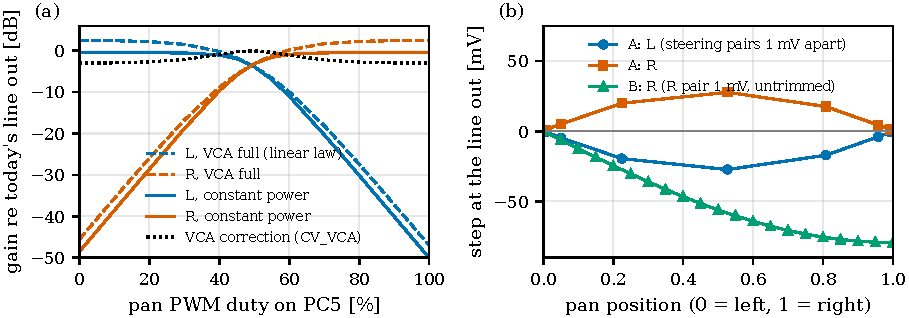
\includegraphics[width=\textwidth]{s13_pan.pdf}
\caption{S13: (a) pan law of variant A over the PC5 duty, with the VCA at full level (linear law) and with the
firmware's constant-power correction; (b) the step at the line out when the VCA opens, for \SI{1}{mV} of mismatch.}
\label{fig:s13}
\end{figure}

\subsection{References and supply}
\begin{itemize}
  \item \textbf{\SI{5}{V} input:} from the backplane (pins 1/2), or from the programmer's \SI{5}{V} through a B5819W
    Schottky diode (no back-feeding into the backplane). On programmer power the card runs at about \SI{4.6}{V};
    S10 (v5c46) shows the same figures there, with the smallest $V_\mathrm{CE}$ at \SI{0.37}{V}.
  \item \textbf{Analog rail VA:} \SI{22}{\ohm} + $3\times\SI{100}{\micro F}$. \SI{47}{\ohm} would halve the inrush but
    cost \SI{0.22}{V} permanently, so \SI{22}{\ohm} stays.
  \item \textbf{MCU:} XC6206 \SI{3.3}{V} LDO. The PWM outputs are duty $\times\,V_\mathrm{DD}$, so the CVs and the DAC
    depend on this rail; their ratios to VREF are absorbed by the calibration.
  \item \textbf{CJ431 pinout:} the SOT-23 CJ431 has the TL432 pinout (1 REF, 2 K, 3 A), not KiCad's TL431DBZ; the
    schematic uses the TL432 symbol.
  \item \textbf{Supply rejection} of the card as built: $-69$ / $-66$ / $-77$\,dB at \SI{100}{Hz} / \SI{1}{kHz} /
    \SI{10}{kHz} (S10 v5c); the CJ431 filter gains 8\,dB at \SI{100}{Hz}.
\end{itemize}

\subsection{MCU pin map}\label{sec:mcu}
The board~1 pin functions carry over: TIM1 and TIM2 keep remap~2 (TIM1\_RM = 0010, TIM2\_RM = 010), USART1 its default
pins. All 18 GPIO of the TSSOP-20 are assigned (Table~\ref{tab:pinsvoice}). Reset is PD7; PA4 is bonded to the same
pin inside the package and is never configured as an output. KiCad's CH32V003 TSSOP-20 symbol fits, as the pinout is
the same.

\begin{table}[htbp]
\centering\footnotesize
\setlength{\tabcolsep}{3.5pt}
\caption{Voice card MCU (\statVoiceMcu, TSSOP-20) pin map: nets from \file{hw/voice.py}, port names from the KiCad
symbol; generated.}\label{tab:pinsvoice}
% generated by gen_tables.py -- do not edit
\begin{tabular}{@{}r l l l @{\hspace{1.2em}} r l l l@{}}
\toprule
Pin & Port & Net & Function & Pin & Port & Net & Function \\
\midrule
1 & PD4 & \texttt{SYNC\_\allowbreak{}IN} & SYNC in (EXTI) & 20 & PD3 & \texttt{PWM\_\allowbreak{}VCA} & TIM1 CH4 $\to$ CV\sub{VCA} \\
2 & PD5 & \texttt{TX\_\allowbreak{}OUT} & USART1 TX $\to$ return line & 19 & PD2 & \texttt{ST\_\allowbreak{}RAIL} & ADC A3: self-test VA/2 \\
3 & PD6 & \texttt{RX\_\allowbreak{}IN} & USART1 RX $\leftarrow$ broadcast & 18 & PD1 & \texttt{SWIO} & SWIO \\
4 & PD7 & \texttt{NRST} & reset (backplane) & 17 & PC7 & \texttt{PWM\_\allowbreak{}CUT} & TIM1 CH2 $\to$ CV\sub{CUT} \\
5 & PA1 & \texttt{CLK\_\allowbreak{}SEL} & clock in (XI, DNP link) & 16 & PC6 & \texttt{PWM\_\allowbreak{}TRIM} & TIM1 CH1 $\to$ VCA trim \\
6 & PA2 & \texttt{ST\_\allowbreak{}VB0} & ADC A0: self-test VB0 & 15 & PC5 & \texttt{PWM\_\allowbreak{}PAN} & TIM2 CH1 $\to$ pan bias \\
7 & VSS & \texttt{GND} & ground & 14 & PC4 & \texttt{ADC\_\allowbreak{}AUDIO} & ADC A2 $\leftarrow$ loopback \\
8 & PD0 & \texttt{LED\_\allowbreak{}PLAY} & LED PLAY & 13 & PC3 & \texttt{LED\_\allowbreak{}STAT} & LED STAT \\
9 & VDD & \texttt{+3V3} & supply & 12 & PC2 & \texttt{PWM\_\allowbreak{}DAC} & TIM2 CH2 $\to$ PWM DAC \\
10 & PC0 & \texttt{PWM\_\allowbreak{}RES} & TIM1 CH3 $\to$ CV\sub{RES} & 11 & PC1 & \texttt{PWM\_\allowbreak{}LO} & TIM2 CH4: DAC low byte \\
\bottomrule
\end{tabular}

\end{table}

\paragraph{DMA.} The V006 has seven DMA channels with fixed request mappings (reference manual table 8-2). The card
uses:
\begin{itemize}
  \item channel~1: the DAC (TIM2 CC3 request, once per carrier period); the ADC therefore runs without DMA;
  \item channel~5: the USART1 receive ring of the voice bus (it shares channel~5 with TIM1\_UP);
  \item channel~4: USART1 transmit (replies on the return line);
  \item channel~2: the CV dither burst (card build): with CCDS = 1 the TIM1 CC1 request comes at each update and
    starts a 4-register burst (CH1CVR--CH4CVR) from a 16-halfword circular table. It replaces the \SI{46.875}{kHz}
    interrupt (about 7\,k cycles per buffer half); board~1 keeps the interrupt for its noise output. (An earlier
    board~1 experiment used channel~6 on the CC3 request.)
\end{itemize}
All three DMA uses (DAC, CV burst, UART ring) ran together on board~1 during a tune: 1353 of 1353 bytes received, no
UART errors, no DAC overruns, CV pattern intact.

\subsection{PCB}\label{sec:voicepcb}
The card is 50\,$\times$\,50\,mm with four layers (Table~\ref{tab:stackvoice}), all parts on the top side:
\begin{itemize}
  \item \textbf{Orientation:} the backplane connector sits centred on the bottom edge. Seen from the part side with the
    connector down, pin~1 is on the right, so the supply and audio pins (1--8) and the analog core are on the right,
    the bus pins (9--16) and the MCU on the left.
  \item \textbf{Top edge:} the three LEDs (power, playing, status), the 1$\times$3 programming header (+5\,V, SWIO, GND,
    the rev 0.1 order) and the 1$\times$3 line-out header (L, R, GND), both right-angle.
  \item \textbf{Passives:} 0402 where the JLCPCB lists have the value; 0603 did not fit (ten parts found no place).
    Values missing in 0402 (\SI{11}{k\ohm}, \SI{240}{k\ohm}, \SI{3.6}{k\ohm}, \SI{620}{\ohm},
    \SI{680}{k\ohm}, \SI{3}{k\ohm}, \SI{30}{k\ohm}, \SI{5.1}{M\ohm}), the \SI{33}{nF} and the \SI{10}{\micro F} bias
    capacitors stay 0603. \statVoiceTp\ test points.
  \item \textbf{Routing:} Freerouting with repair passes and pre-routes (SWIO along the left and bottom edges, the
    VCA collectors into the steering pairs). The routed board has \statVoiceFootprints\ footprints,
    \statVoiceSegments\ track segments (\statVoiceLenF\,m on F.Cu, \statVoiceLenB\,m on B.Cu) and \statVoiceVias\
    vias. The KiCad DRC reports 0 errors and 0 unconnected pads; the remaining warnings are the three locally
    modified header footprints.
  \item \textbf{Known weak spot:} VREF (\SI{128}{mm}) and the VBIAS divider node (\SI{102}{mm}) are long tracks; a
    VREF region on In2 is a candidate for the next revision.
\end{itemize}

\begin{table}[htbp]
\centering\small
\caption{Voice card layer stack (JLCPCB standard 4-layer, 1.6\,mm).}\label{tab:stackvoice}
\begin{tabularx}{\textwidth}{@{}l X@{}}
\toprule
Layer & Use \\
\midrule
F.Cu & all parts, signals \\
In1.Cu & solid GND \\
In2.Cu & supply planes: VA under the analog part, +3V3 under the MCU and the top edge, +5V in a strip along the right
  and bottom edges \\
B.Cu & signals only \\
\bottomrule
\end{tabularx}
\end{table}

\begin{figure}[p]
\centering
\begin{subfigure}{0.48\textwidth}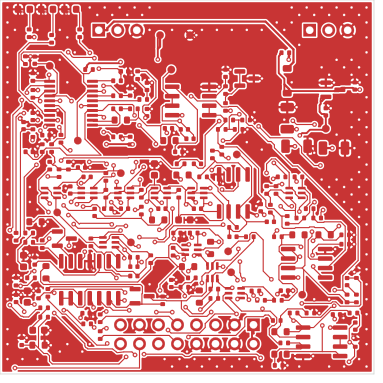
\includegraphics[width=\linewidth]{voice_pcb/fcu.png}\caption{F.Cu}\end{subfigure}\hfill
\begin{subfigure}{0.48\textwidth}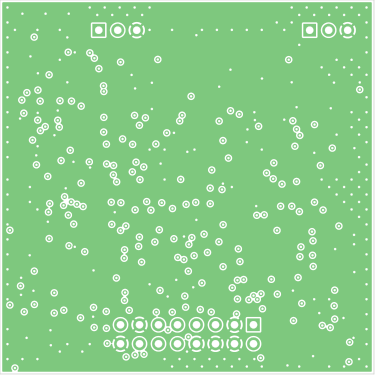
\includegraphics[width=\linewidth]{voice_pcb/in1.png}\caption{In1.Cu (GND)}\end{subfigure}\\[6pt]
\begin{subfigure}{0.48\textwidth}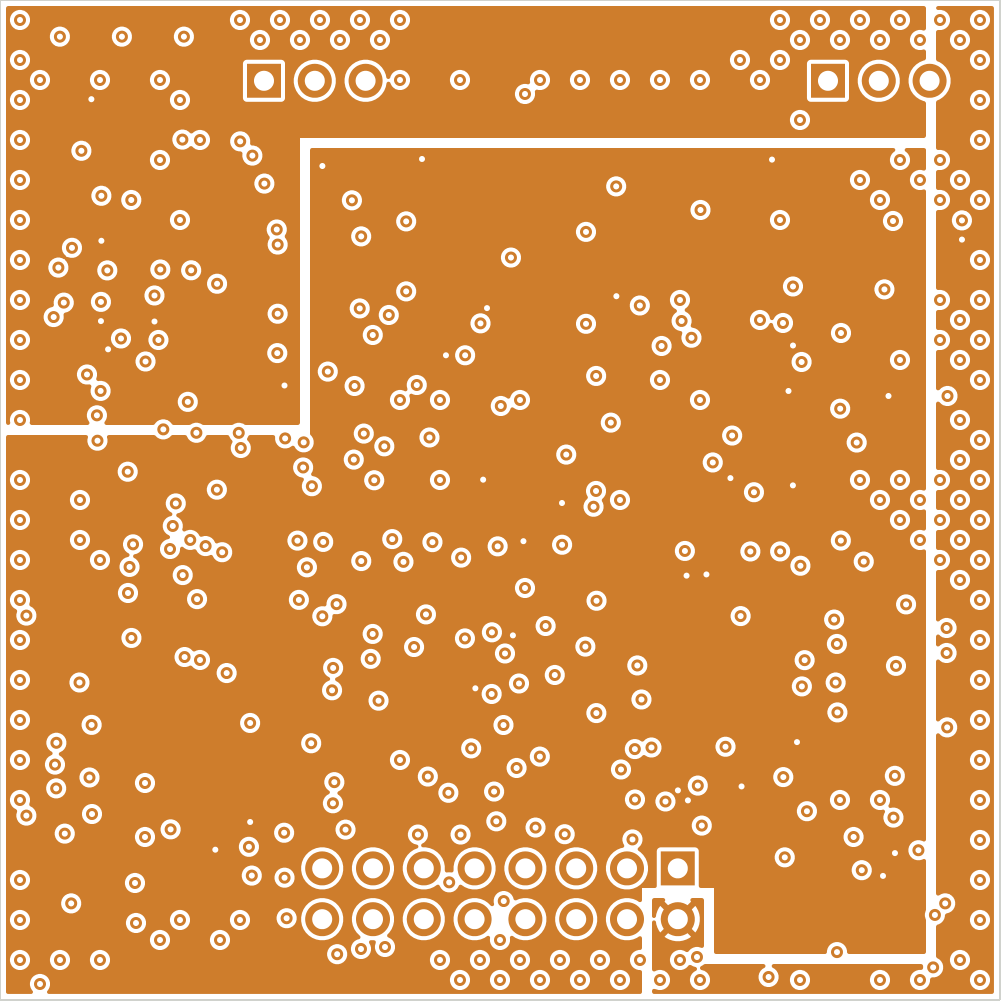
\includegraphics[width=\linewidth]{voice_pcb/in2.png}\caption{In2.Cu (VA / +3V3 / +5V)}\end{subfigure}\hfill
\begin{subfigure}{0.48\textwidth}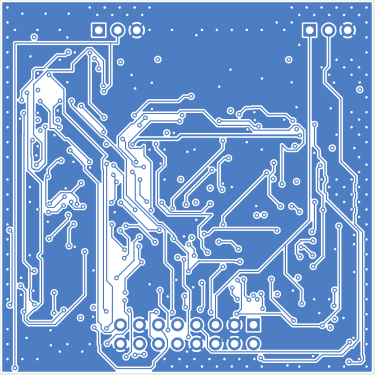
\includegraphics[width=\linewidth]{voice_pcb/bcu.png}\caption{B.Cu}\end{subfigure}
\caption{Voice card copper layers, seen from the top (\file{docs/figures/voice\_pcb/}).}\label{fig:voicelayers}
\end{figure}

\begin{figure}[p]
\centering
\begin{subfigure}{0.48\textwidth}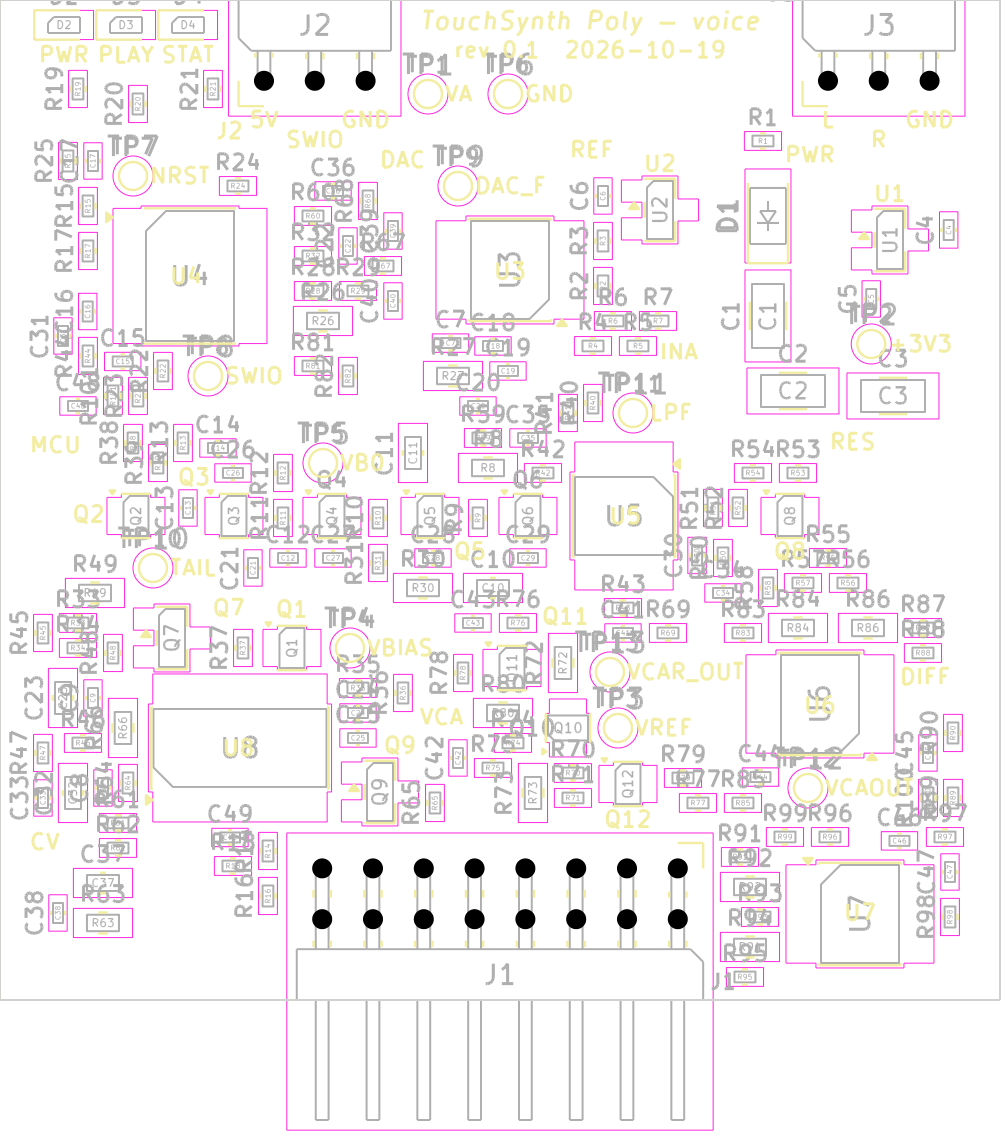
\includegraphics[width=\linewidth]{voice_pcb/place.png}\caption{placement (silk, fab, courtyards)}\end{subfigure}\hfill
\begin{subfigure}{0.48\textwidth}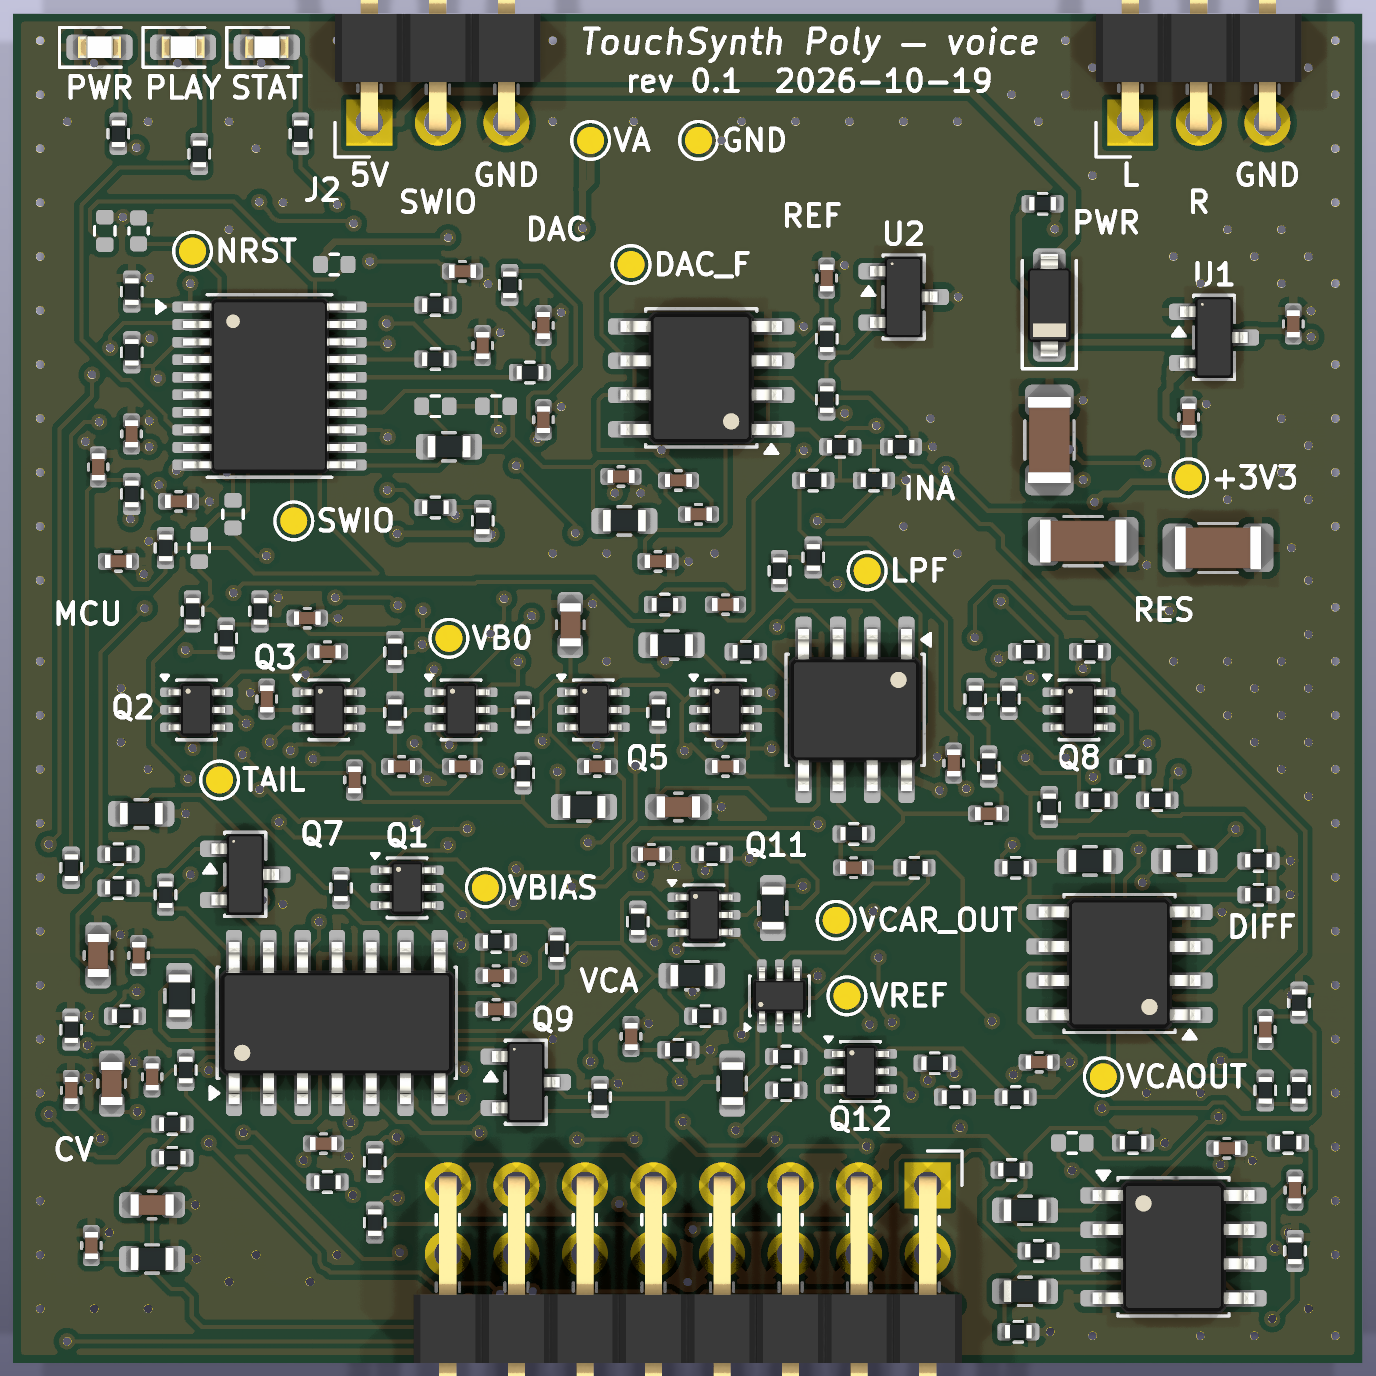
\includegraphics[width=\linewidth]{voice_pcb/render_top.png}\caption{3D render, top}\end{subfigure}\\[6pt]
\begin{subfigure}{0.48\textwidth}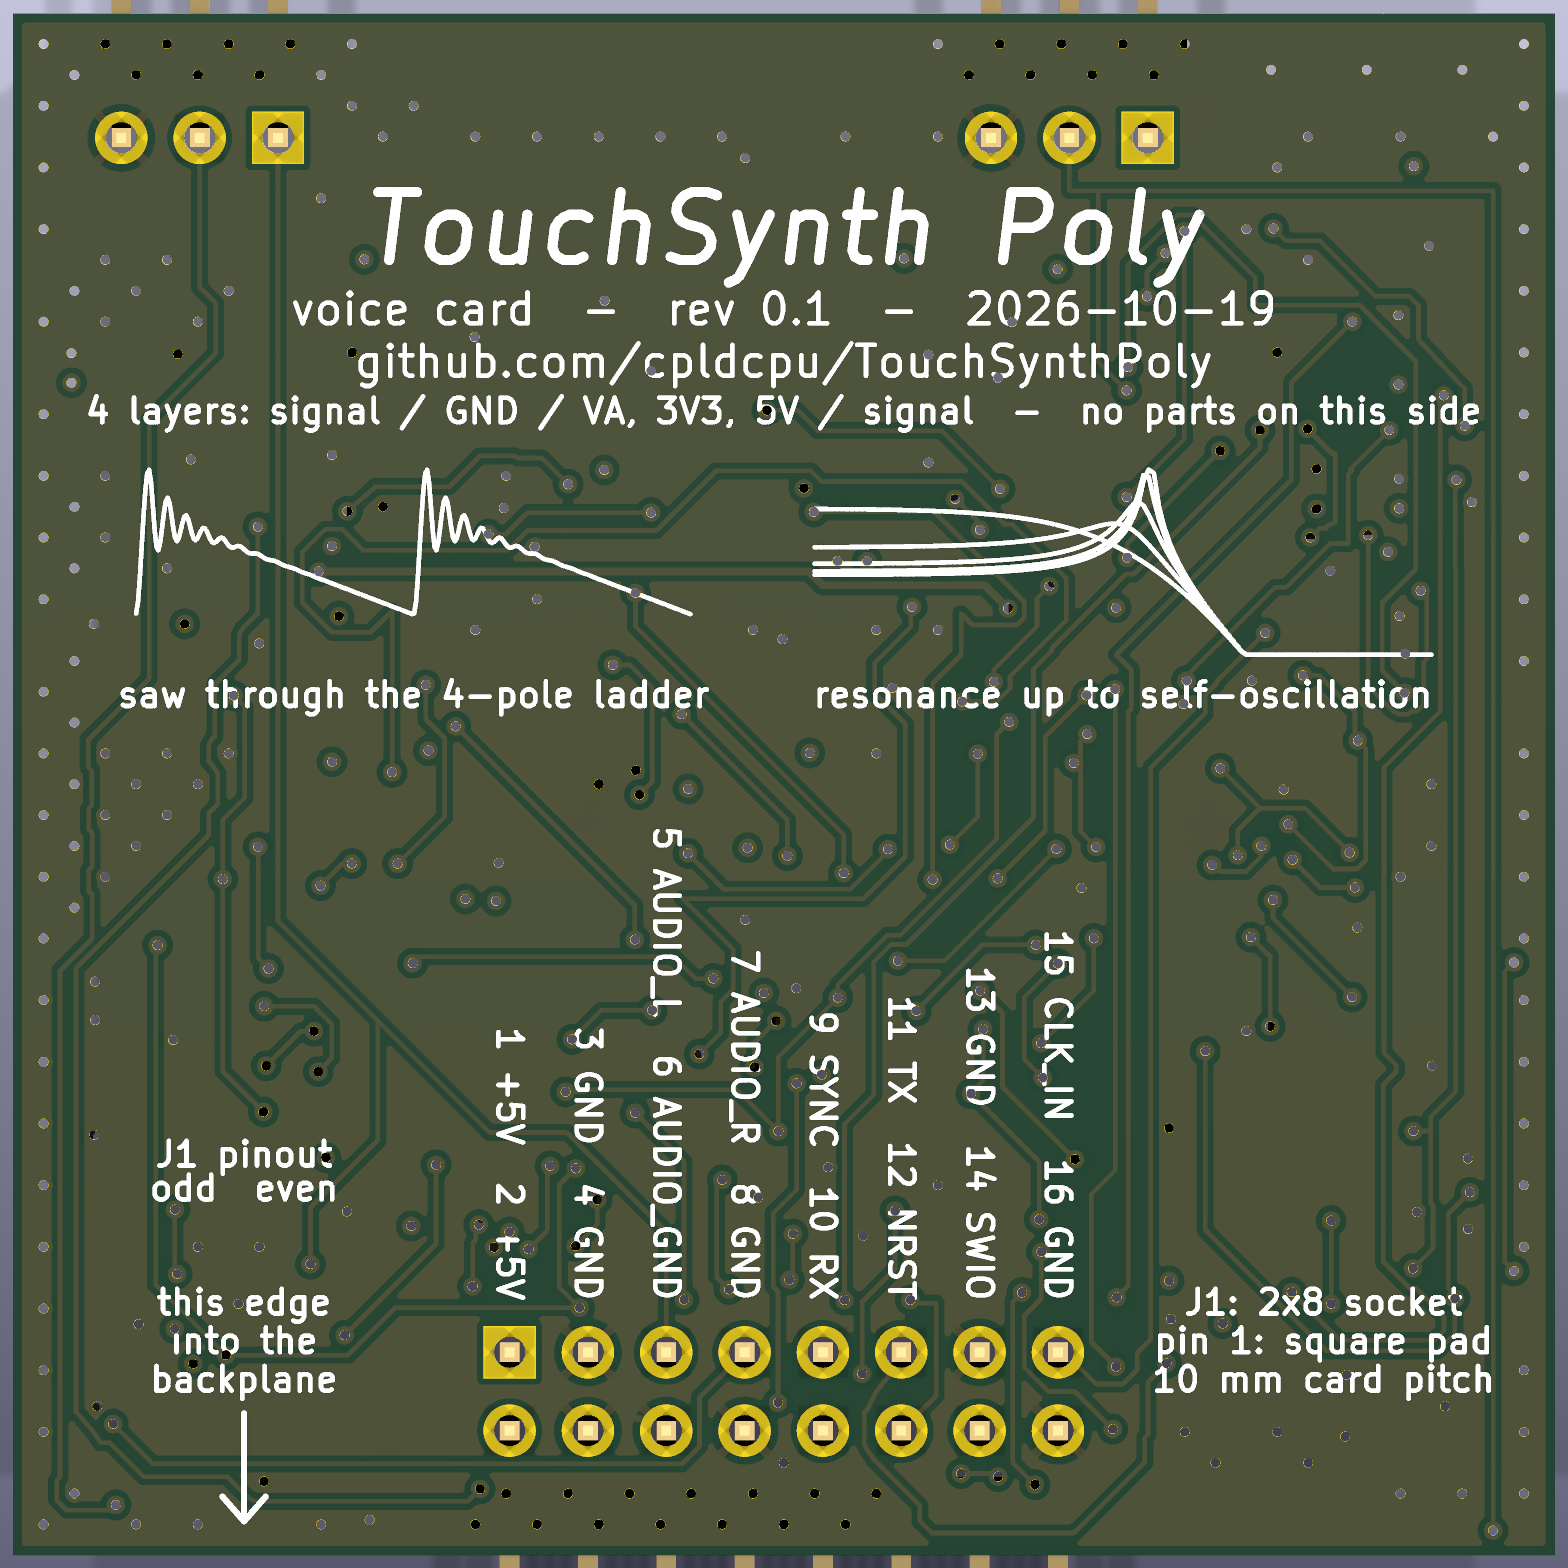
\includegraphics[width=\linewidth]{voice_pcb/render_bottom.png}\caption{3D render, bottom}\end{subfigure}\hfill
\begin{subfigure}{0.48\textwidth}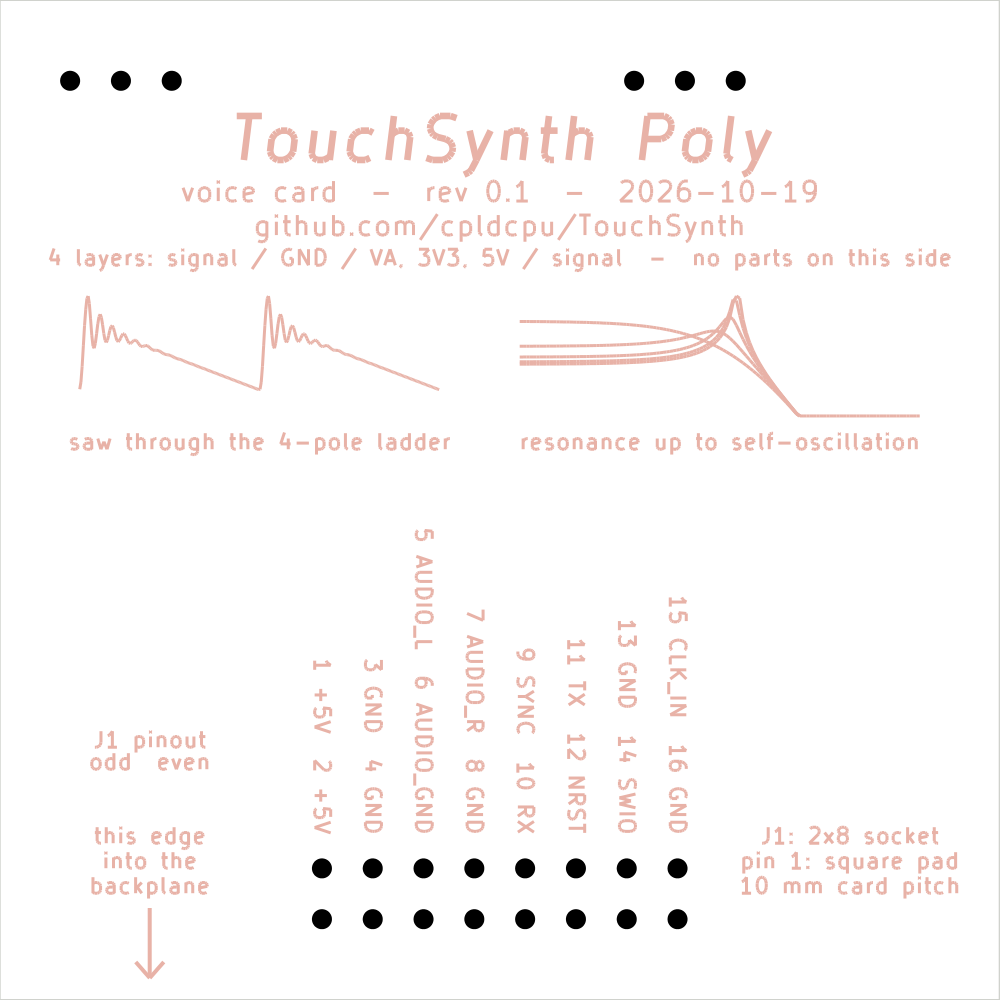
\includegraphics[width=\linewidth]{voice_pcb/bsilk.png}\caption{bottom silkscreen (seen from the back)}\end{subfigure}
\caption{Voice card placement and renders.}\label{fig:voicerender}
\end{figure}

% =====================================================================================================================
\section{Backplane}\label{sec:bp}

\subsection{Overview}
The backplane (\file{hw/backplane.py}, \statBpSheets\ schematic sheets, \statBpParts\ parts) carries the controller,
power, USB, the voice bus with eight slots and the mixer (Figure~\ref{fig:bpblock}). The sensitive parts stay small
and local: the cards bring their own references and regulators, so the backplane carries only \SI{5}{V}, ground and
line-level audio. The design follows \file{docs/backplane.md}, status 0.3.

\begin{figure}[htbp]
\centering
\resizebox{\textwidth}{!}{%
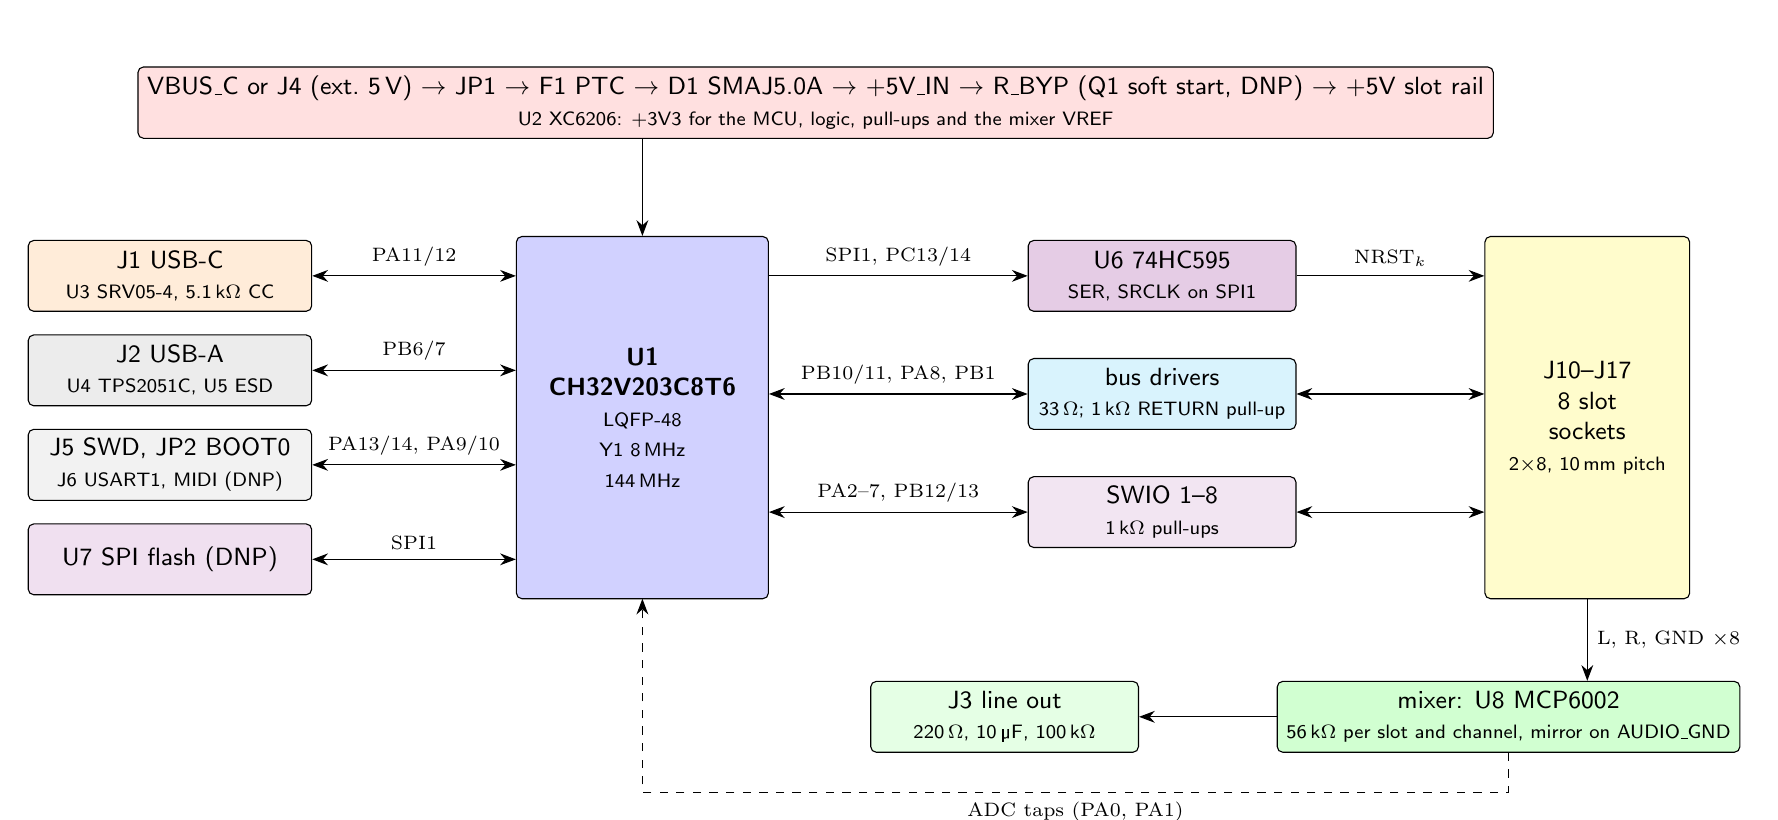
\begin{tikzpicture}[font=\small\sffamily, >={Stealth[length=2mm]},
  blk/.style={draw, rounded corners=2pt, fill=#1, minimum height=9mm, align=center}, blk/.default=white,
  lab/.style={font=\scriptsize, above}]
  \node[blk=red!12, minimum width=150mm] (pwr) at (8.2,4.0)
    {VBUS\_C or J4 (ext.\ 5\,V) $\to$ JP1 $\to$ F1 PTC $\to$ D1 SMAJ5.0A $\to$ +5V\_IN $\to$ R\_BYP (Q1 soft start, DNP)
     $\to$ +5V slot rail\\\scriptsize U2 XC6206: +3V3 for the MCU, logic, pull-ups and the mixer VREF};
  \node[blk=blue!18, minimum width=32mm, minimum height=46mm] (mcu) at (6,0)
    {\textbf{U1}\\\textbf{CH32V203C8T6}\\\scriptsize LQFP-48\\\scriptsize Y1 8\,MHz\\\scriptsize 144\,MHz};
  \node[blk=orange!15, minimum width=36mm] (usbc) at (0,1.8) {J1 USB-C\\\scriptsize U3 SRV05-4, 5.1\,k$\Omega$ CC};
  \node[blk=gray!15, minimum width=36mm] (usba) at (0,0.6) {J2 USB-A\\\scriptsize U4 TPS2051C, U5 ESD};
  \node[blk=gray!10, minimum width=36mm] (prog) at (0,-0.6) {J5 SWD, JP2 BOOT0\\\scriptsize J6 USART1, MIDI (DNP)};
  \node[blk=violet!12, minimum width=36mm] (flash) at (0,-1.8) {U7 SPI flash (DNP)};
  \draw[<->] (usbc.east) -- node[lab]{PA11/12} (usbc.east -| mcu.west);
  \draw[<->] (usba.east) -- node[lab]{PB6/7} (usba.east -| mcu.west);
  \draw[<->] (prog.east) -- node[lab]{PA13/14, PA9/10} (prog.east -| mcu.west);
  \draw[<->] (flash.east) -- node[lab]{SPI1} (flash.east -| mcu.west);
  \node[blk=violet!20, minimum width=34mm] (sr) at (12.6,1.8) {U6 74HC595\\\scriptsize SER, SRCLK on SPI1};
  \node[blk=cyan!15, minimum width=34mm] (bus) at (12.6,0.3) {bus drivers\\\scriptsize 33\,$\Omega$; 1\,k$\Omega$ RETURN pull-up};
  \node[blk=violet!10, minimum width=34mm] (swio) at (12.6,-1.2) {SWIO 1--8\\\scriptsize 1\,k$\Omega$ pull-ups};
  \draw[->] (sr.west -| mcu.east) -- node[lab]{SPI1, PC13/14} (sr.west);
  \draw[<->] (bus.west -| mcu.east) -- node[lab]{PB10/11, PA8, PB1} (bus.west);
  \draw[<->] (swio.west -| mcu.east) -- node[lab]{PA2--7, PB12/13} (swio.west);
  \node[blk=yellow!20, minimum width=26mm, minimum height=46mm] (slots) at (18.0,0)
    {J10--J17\\8 slot\\sockets\\\scriptsize 2$\times$8, 10\,mm pitch};
  \draw[->] (sr.east) -- node[lab]{NRST$_k$} (sr.east -| slots.west);
  \draw[<->] (bus.east) -- (bus.east -| slots.west);
  \draw[<->] (swio.east) -- (swio.east -| slots.west);
  \node[blk=green!18, minimum width=44mm] (mix) at (17.0,-3.8) {mixer: U8 MCP6002\\\scriptsize 56\,k$\Omega$ per slot and
    channel, mirror on AUDIO\_GND};
  \draw[->] (slots.south -| 18.0,0) -- node[right,font=\scriptsize]{L, R, GND $\times$8} (mix.north -| 18.0,0);
  \node[blk=green!10, minimum width=34mm] (out) at (10.6,-3.8) {J3 line out\\\scriptsize 220\,$\Omega$, 10\,\textmu F,
    100\,k$\Omega$};
  \draw[->] (mix) -- (out);
  \draw[->, dashed] (mix.south) -- ++(0,-0.5) -| node[pos=0.25,below,font=\scriptsize]{ADC taps (PA0, PA1)} (6.0,-2.3);
  \draw[->] (pwr.south -| 6.0,0) -- (mcu.north);
\end{tikzpicture}}
\caption{Backplane blocks with the controller pins they use.}
\label{fig:bpblock}
\end{figure}

\subsection{Controller and pin map}
The CH32V203C8T6 (\SI{64}{KB} flash, \SI{20}{KB} SRAM) runs from its \SI{8}{MHz} crystal at \SI{144}{MHz}: HCLK
\SI{144}{MHz}, PCLK1 = PCLK2 = \SI{72}{MHz}, so USART3 divides exactly to \SI{1}{Mbaud} and TIM3 gives exactly
\SI{24}{MHz} for the clock option. \statBpGpioUsed\ of its 37 GPIO are used; \statBpGpioFree\ (PC15, PB0, PB14) are
left as test pads. Table~\ref{tab:pinsbp} gives the pin map; the full rationale is in \file{docs/backplane.md}~3.
The main decisions:
\begin{itemize}
  \item \textbf{Bench pins kept:} USART3 (PB10 TX, PB11 RX) for the bus, SYNC on PA8 (TIM1 CH1), USART1 (PA9/PA10)
    free for the bootloader and a debug UART, SWD on PA13/PA14.
  \item \textbf{CLK\_IN from a timer, not MCO:} MCO exists only on PA8 (taken by SYNC) and can only give 8 or
    \SI{72}{MHz}. The V006's PLL is a fixed $\times$2, so a card on the external clock needs \SI{24}{MHz}: TIM3 CH4 on
    PB1 with ARR = 5 gives exactly that, locked to the crystal.
  \item \textbf{SPI1 remap 1} (PA15, PB3, PB4, PB5) for the flash and the 74HC595, so that the default SPI1 pins
    PA4--PA7 stay free for SWIO.
  \item \textbf{BOOT1 (PB2)} must be low at reset for the bootloader, so it drives the activity LED with a
    \SI{10}{k\ohm} pull-down; a slot line or VBUS\_DET cannot sit there.
  \item \textbf{PC13--PC15} source no current and switch at \SI{2}{MHz} at most; they carry the 595's latch and output
    enable only.
  \item \textbf{MIDI DIN} (not fitted) shares USART1 RX (PA10) with the debug header through jumper JP3, as none of the
    free pins is a USART RX.
  \item \textbf{5\,V tolerance:} the USB pins are protected by SRV05-4 arrays; SYNC, RETURN and SWIO 7/8 are on 5\,V
    tolerant pins, SWIO 1--6 are not. Only a card plugged in reversed could drive them; the card guides are meant to
    prevent that mechanically.
\end{itemize}

\begin{table}[htbp]
\centering\scriptsize
\setlength{\tabcolsep}{2.6pt}
\caption{Controller (CH32V203C8T6, LQFP-48) pin map: nets from \file{hw/backplane.py}, port names from the KiCad
symbol; generated.}\label{tab:pinsbp}
% generated by gen_tables.py -- do not edit
\begin{tabular}{@{}r l l l @{\hspace{1em}} r l l l@{}}
\toprule
Pin & Port & Net & Use & Pin & Port & Net & Use \\
\midrule
1 & VBAT & \texttt{+3V3} & supply & 25 & PB12 & \texttt{SWIO\_\allowbreak{}7} & SWIO slot 7 \\
2 & PC13 & \texttt{SR\_\allowbreak{}LATCH} & 595 latch (RCLK) & 26 & PB13 & \texttt{SWIO\_\allowbreak{}8} & SWIO slot 8 \\
3 & PC14 & \texttt{SR\_\allowbreak{}OE\_\allowbreak{}N} & 595 output enable & 27 & PB14 & \texttt{PB14} & free (test pad) \\
4 & PC15 & \texttt{PC15} & free (test pad) & 28 & PB15 & \texttt{VBUS\_\allowbreak{}DET} & USB-C VBUS sense \\
5 & OSC\_IN & \texttt{OSC\_\allowbreak{}IN} & 8\,MHz crystal & 29 & PA8 & \texttt{SYNC\_\allowbreak{}O} & TIM1 CH1: SYNC 1\,kHz \\
6 & OSC\_OUT & \texttt{OSC\_\allowbreak{}OUT} & 8\,MHz crystal & 30 & PA9 & \texttt{UART\_\allowbreak{}TX} & USART1 TX (J6) \\
7 & NRST & \texttt{MCU\_\allowbreak{}NRST} & MCU reset & 31 & PA10 & \texttt{UART\_\allowbreak{}RX} & USART1 RX (J6, MIDI) \\
8 & VSSA & \texttt{GND} & ground & 32 & PA11 & \texttt{USBD\_\allowbreak{}DM} & USB device D$-$ \\
9 & VDDA & \texttt{VDDA} & analog supply (ferrite) & 33 & PA12 & \texttt{USBD\_\allowbreak{}DP} & USB device D+ \\
10 & PA0 & \texttt{ADC\_\allowbreak{}L} & ADC1 IN0 $\leftarrow$ mix L & 34 & SWDIO & \texttt{SWDIO} & SWD (J5) \\
11 & PA1 & \texttt{ADC\_\allowbreak{}R} & ADC2 IN1 $\leftarrow$ mix R & 35 & VSS & \texttt{GND} & ground \\
12 & PA2 & \texttt{SWIO\_\allowbreak{}1} & SWIO slot 1 & 36 & VDD & \texttt{+3V3} & supply \\
13 & PA3 & \texttt{SWIO\_\allowbreak{}2} & SWIO slot 2 & 37 & SWCLK & \texttt{SWCLK} & SWD (J5) \\
14 & PA4 & \texttt{SWIO\_\allowbreak{}3} & SWIO slot 3 & 38 & PA15 & \texttt{FLASH\_\allowbreak{}CS\_\allowbreak{}N} & flash CS (GPIO) \\
15 & PA5 & \texttt{SWIO\_\allowbreak{}4} & SWIO slot 4 & 39 & PB3 & \texttt{SPI\_\allowbreak{}SCK} & SPI1 SCK: flash, 595 \\
16 & PA6 & \texttt{SWIO\_\allowbreak{}5} & SWIO slot 5 & 40 & PB4 & \texttt{SPI\_\allowbreak{}MISO} & SPI1 MISO: flash \\
17 & PA7 & \texttt{SWIO\_\allowbreak{}6} & SWIO slot 6 & 41 & PB5 & \texttt{SPI\_\allowbreak{}MOSI} & SPI1 MOSI: flash, 595 \\
18 & PB0 & \texttt{PB0} & free (test pad) & 42 & PB6 & \texttt{USBH\_\allowbreak{}DM} & USB host D$-$ \\
19 & PB1 & \texttt{CLK\_\allowbreak{}O} & TIM3 CH4: 24\,MHz (option) & 43 & PB7 & \texttt{USBH\_\allowbreak{}DP} & USB host D+ \\
20 & PB2 & \texttt{LED\_\allowbreak{}ACT} & activity LED (BOOT1) & 44 & BOOT0 & \texttt{BOOT0} & boot select (JP2) \\
21 & PB10 & \texttt{BCAST\_\allowbreak{}O} & USART3 TX: broadcast & 45 & PB8 & \texttt{HOST\_\allowbreak{}EN} & host switch enable \\
22 & PB11 & \texttt{RETURN} & USART3 RX: return line & 46 & PB9 & \texttt{HOST\_\allowbreak{}FLT\_\allowbreak{}N} & host switch fault \\
23 & VSS & \texttt{GND} & ground & 47 & VSS & \texttt{GND} & ground \\
24 & VDD\_VIO & \texttt{+3V3} & supply & 48 & VDD & \texttt{+3V3} & supply \\
\bottomrule
\end{tabular}

\end{table}

\subsection{Power entry and soft-start option}\label{sec:bppower}
\begin{itemize}
  \item \textbf{Source:} USB-C VBUS (sink, \SI{5.1}{k\ohm} on CC1 and CC2) or an external \SI{5}{V} adapter on J4,
    selected by a 3-pin jumper JP1. A jumper instead of diodes avoids a diode drop, which the cards' supply margin
    could not afford. With the external supply selected, VBUS only feeds the VBUS sense divider (self-powered device).
  \item \textbf{Protection:} a \SI{0.75}{A} PTC (hand-soldered; none on the lists) followed by an SMAJ5.0A TVS: an
    overvoltage or a reversed external supply makes the TVS conduct and the PTC trip.
  \item \textbf{\SI{3.3}{V}:} an XC6206 (\SI{200}{mA}, load about \SI{30}{mA}) from +5V\_IN for the MCU, the logic, the
    pull-ups and the mixer's VREF.
  \item \textbf{Slot rail:} $2\times\SI{47}{\micro F}$ at the rail and \SI{10}{\micro F} at each socket.
  \item \textbf{Soft start (not fitted):} an AO3401A P-channel MOSFET between +5V\_IN and the slot rail, bridged by a
    \SI{0}{\ohm} 1206 resistor R\_BYP. If a port or hub drops out at plug-in, R\_BYP is removed and Q1 fitted with
    $R_{GS} = \SI{1}{M\ohm}$, $R_G = \SI{220}{k\ohm}$ to ground and $C_{GD} = \SI{100}{nF}$. By hand estimate the drain
    then ramps at about \SI{116}{V/s} (\SI{5}{V} in about \SI{40}{ms}), the charging current of the slot capacitance
    (about \SI{0.95}{mF}) stays near \SI{110}{mA}, and $R_{DS(on)}$ of about \SI{60}{m\ohm} costs \SI{30}{mV} at
    \SI{0.5}{A}. This estimate is to be simulated before the option is used (proposed S14).
  \item \textbf{VBUS sense:} \SI{22}{k\ohm} / \SI{33}{k\ohm} to PB15 (\SI{3.0}{V} at \SI{5.0}{V}), so the device
    enables its D+ pull-up only with a computer present.
\end{itemize}

\subsection{USB device and host}
\begin{itemize}
  \item \textbf{Device} on USBD (PA11/PA12) through \SI{0}{\ohm} series positions: a composite of class-compliant
    USB-MIDI, CDC (configuration, presets, firmware, a bridge to each card's console) and, as an option, UAC1 audio
    input of the mix. Full speed needs no controlled impedance at this length. The USBD D+ pull-up is inside the
    chip: the USBD driver enumerated on it alone against the V203's own USBFS host (bench, 20 October); a
    \SI{1.5}{k\ohm} footprint stays as an unfitted fallback.
  \item \textbf{Host} on USBFS (PB6/PB7), so device and host run at the same time. The port is fitted (since 20 October
    2026; it was first left unfitted): TPS2051C current-limited switch (SOT-23-5, fixed \SI{0.5}{A}, hand-soldered: no such
    switch on the lists), USB-A receptacle, ESD array, $2\times\SI{47}{\micro F}$ on VBUS\_HOST (about
    \SI{40}{\micro F} at \SI{5}{V} against the \SI{120}{\micro F} USB 2.0 asks for), enable (PB8, \SI{100}{k\ohm}
    pull-down: off until the firmware decides) and fault (PB9, open drain, red LED). Host-mode pull-downs on D+/D$-$
    exist inside: on the development board's USBFS (the same pins) they measure about 13--15\,k$\Omega$ against a
    PC's pull-downs; the two \SI{15}{k\ohm} footprints stay unfitted.
\end{itemize}

\subsection{Voice bus drivers, NRST and SWIO}
\begin{itemize}
  \item \textbf{Broadcast} (USART3 TX, push-pull) and \textbf{SYNC} (TIM1 CH1) through \SI{33}{\ohm} series resistors
    to every slot; the \textbf{return line} (USART3 RX) with a \SI{1}{k\ohm} pull-up (the cards drive it open drain;
    about \SI{0.3}{\micro s} rise time on \SI{150}{pF}, against a \SI{1}{\micro s} bit). The \SI{24}{MHz} CLK line has
    its own \SI{33}{\ohm} resistor and is off by default.
  \item \textbf{NRST through a 74HC595} (Table~\ref{tab:slots}). The eight NRST lines come from the outputs of U6, whose
    SER and SRCLK share SPI1 with the flash; RCLK and OE are GPIOs. The outputs drive NRST directly, without series
    resistors or pull-downs. At power-up the storage register is undefined, so a \SI{10}{k\ohm} pull-up on OE keeps
    the outputs off until the firmware has shifted zeros in and drives OE low. While the controller is in reset, in
    its bootloader or halted, the NRST lines float and the cards run standalone; the firmware takes them back through
    the 595 or over SWIO. Every flash transfer also clocks the 595's shift register, so the firmware always shifts all
    8 bits directly before a latch.
  \item \textbf{SWIO:} each slot has its own SWIO line from a controller GPIO with a \SI{1}{k\ohm} pull-up: the card has
    none, and the one-wire protocol samples about \SI{0.6}{\micro s} after each edge. On the bench, without a pull-up,
    every read returned 0. Until the controller programs the cards, each card's own programming header stays
    reachable at its top edge; there is no SWIO header on the backplane.
\end{itemize}

\begin{table}[htbp]
\centering\small
\caption{Slot lines (generated from \file{hw/backplane.py}).}\label{tab:slots}
% generated by gen_tables.py -- do not edit
\begin{tabular}{@{}l l l l l@{}}
\toprule
Slot & Socket & NRST (pin 12) & SWIO (pin 14) & SWIO pull-up \\
\midrule
1 & J10 & U6 QA (pin 15) & PA2 (pin 12) & RN1, 1\,k$\Omega$ \\
2 & J11 & U6 QB (pin 1) & PA3 (pin 13) & RN1, 1\,k$\Omega$ \\
3 & J12 & U6 QC (pin 2) & PA4 (pin 14) & RN1, 1\,k$\Omega$ \\
4 & J13 & U6 QD (pin 3) & PA5 (pin 15) & RN1, 1\,k$\Omega$ \\
5 & J14 & U6 QE (pin 4) & PA6 (pin 16) & RN2, 1\,k$\Omega$ \\
6 & J15 & U6 QF (pin 5) & PA7 (pin 17) & RN2, 1\,k$\Omega$ \\
7 & J16 & U6 QG (pin 6) & PB12 (pin 25) & RN2, 1\,k$\Omega$ \\
8 & J17 & U6 QH (pin 7) & PB13 (pin 26) & RN2, 1\,k$\Omega$ \\
\bottomrule
\end{tabular}

\end{table}

\subsection{Two-bus stereo mixer (S12)}\label{sec:mixer}
Figure~\ref{fig:mixer} shows one channel with one slot. Two MCP6002 inverting summing amplifiers (one package, U8) add
the left and the right outputs of all slots. Every slot has the same seven parts; the pan is on the cards.
\begin{itemize}
  \item \textbf{Per slot:} AUDIO\_L and AUDIO\_R each through \SI{10}{\micro F} and \SI{56}{k\ohm} into the L and R
    summing nodes. The input capacitors keep the cards' \SI{100}{k\ohm} output bleeders off the \SI{2.4}{V} summing
    nodes; without them the outputs would sit at \SI{4.9}{V} (S12).
  \item \textbf{Pseudo-differential input:} AUDIO\_GND of each slot goes through one \SI{10}{\micro F} (shared by L and R)
    to node $Y_k$, and from there through \SI{56}{k\ohm} to each amplifier's + input. Each + input has
    \SI{20}{k\ohm}\,$\parallel$\,\SI{47}{pF} to VREF, mirroring the feedback network $R_F$ = \SI{20}{k\ohm}\,$\parallel$\,\SI{47}{pF}. Hence
    \begin{equation}
      v_\mathrm{out} = V_\mathrm{REF} - 0.357 \sum_k \left(v_{\mathrm{AUDIO},k} - v_{\mathrm{AUDIO\_GND},k}\right)
    \end{equation}
    for any set of populated slots: ground currents along the backplane do not add to the audio.
  \item \textbf{Gain:} \statStwelveGain\ per card, sized so that 8 cards hard-panned in phase at the capped level
    (\statStwelveCardHard\,V\sub{pp} each) give \statStwelveHard\,V\sub{pp}, \statStwelveHardMargin\,dB below clipping.
    Without the firmware cap on CV\sub{VCA} (\statStwelveCardUncapped\,V\sub{pp} per card) 8 hard-panned cards would
    clip.
  \item \textbf{Op-amp rail:} \SI{47}{\ohm} + \SI{22}{\micro F} from the slot rail. The MCP6002 rejects supply noise
    poorly at the noise gain of 3.9 that eight inputs give.
  \item \textbf{Line out} on the west edge: \SI{220}{\ohm} + \SI{10}{\micro F} per channel to a \SI{3.5}{mm} stereo jack,
    \SI{100}{k\ohm} bleeder. The mixer, the line-out stage and the jack sit together at the west end of the slot row,
    so the line-out run is short.
  \item \textbf{ADC taps} (USB audio option): \SI{15}{k\ohm} / \SI{27}{k\ohm} with \SI{330}{pF} C0G at PA0 / PA1. The
    V203's two ADCs in dual mode at \SI{384}{kHz}, decimated by 8, keep the \SI{187.5}{kHz} carrier out of the band
    (\SI{-111}{dBFS}). The internal ADC limits this path to about \SI{60}{dB} signal-to-noise for one centred card.
\end{itemize}

\begin{figure}[htbp]
\centering
\begin{circuitikz}[scale=0.72, transform shape, font=\small]
  \draw (8,0) node[op amp](OA){\scriptsize U8A};
  % inverting side
  \draw (OA.-) -- (6.4,0.5) coordinate(nm);
  \draw (nm) to[R, l_=56\,k$\Omega$, *-] (4.0,0.5) to[C, l_=10\,\textmu F, -o] (1.4,0.5) node[left]{AUDIO\_L$_k$};
  \draw (nm) -- (6.4,2.0) to[R, l=20\,k$\Omega$] (9.8,2.0) -- (9.8,0);
  \draw (6.4,2.0) -- (6.4,3.4) to[C, l=47\,pF] (9.8,3.4) -- (9.8,2.0);
  \draw (OA.out) -- (9.8,0) node[circ]{} -- (10.6,0) node[circ]{} node[above]{MIX\_L};
  % non-inverting side
  \draw (OA.+) -- (6.4,-0.5) coordinate(np);
  \draw (np) to[R, l=56\,k$\Omega$, *-*] (4.0,-0.5) coordinate(y) to[C, l=10\,\textmu F, -o] (1.4,-0.5)
        node[left]{AUDIO\_GND$_k$};
  \node[above left] at (y) {$Y_k$};
  \draw (y) to[R, l=56\,k$\Omega$, -o] (4.0,-3.0) node[below]{to R+};
  \draw (np) -- (6.4,-1.4) coordinate(vt);
  \draw (vt) to[R, l_=20\,k$\Omega$] (6.4,-3.4) coordinate(vr);
  \draw (vt) -- (7.8,-1.4) to[C, l=47\,pF] (7.8,-3.4) -- (vr);
  \draw (vr) node[circ]{};
  \node[left] at (6.3,-3.75) {VREF};
  % VREF generation: +3V3 -> 10k -> (27k, 10u) -> 10k -> VREF (10u)
  \draw (vr) -- (6.4,-4.2) to[C, l_=10\,\textmu F] (6.4,-5.9) node[ground]{};
  \draw (6.4,-4.2) to[R, l=10\,k$\Omega$, *-*] (9.4,-4.2) coordinate(va) to[R, l=10\,k$\Omega$, -o] (12.6,-4.2)
        node[right]{+3V3};
  \draw (va) to[R, l_=27\,k$\Omega$] (9.4,-5.9) node[ground]{};
  \draw (va) -- (10.8,-4.2) to[C, l=10\,\textmu F] (10.8,-5.9) node[ground]{};
  % output
  \draw (10.6,0) to[R, l=220\,$\Omega$] (12.8,0) to[C, l=10\,\textmu F, -*] (15.0,0) -- (15.6,0) node[right]{LINE\_L (J3)};
  \draw (15.0,0) to[R, l=100\,k$\Omega$] (15.0,-2.0) node[ground]{};
  % per-slot box
  \draw[dashed, blue!60!black, rounded corners] (-2.9,-3.9) rectangle (5.2,1.5);
  \node[blue!60!black, font=\scriptsize, anchor=north west] at (-2.8,-4.0) {per slot $k$ = 1\ldots8 (R channel alike)};
\end{circuitikz}
\caption{Mixer, left channel, one slot drawn. AUDIO\_L of every slot sums into the $-$ input; AUDIO\_GND of every slot
is mirrored onto the $+$ input through the same resistor value, and node $Y_k$ also feeds the right channel's $+$
input. VREF comes from the controller's +3V3 through two RC stages, unbuffered. The ADC tap (\SI{15}{k\ohm} /
\SI{27}{k\ohm}, \SI{330}{pF}) on MIX\_L is not drawn.}
\label{fig:mixer}
\end{figure}

\paragraph{Simulation (S12).} Table~\ref{tab:s12} and Figure~\ref{fig:s12} give the results of the two-bus mixer with
all 8 slots populated. The mirror network rejects ground differences by \SI{65}{dB} nominally at \SI{1}{kHz}; with
1\,\% resistors the worst case is about \SI{29}{dB} and the typical case \SI{45}{dB}. The shared \SI{10}{\micro F}
mirror capacitor per slot is needed: \SI{4.7}{\micro F} would halve the low-frequency ground rejection. With separate
L and R pins the crosstalk between the channels is below \SI{-105}{dB}, with or without empty slots.

\begin{table}[htbp]
\centering\small
\caption{S12: two-bus mixer, 8 slots (\file{docs/results/s12\_mixer\_2bus.csv}); generated.}\label{tab:s12}
% generated by gen_tables.py -- do not edit
\begin{tabular}{@{}l l@{}}
\toprule
Quantity & Simulated \\
\midrule
Gain per card (56\,k$\Omega$ into 20\,k$\Omega$) & 0.357 \\
8 cards hard left, in phase, capped level & 3.95\,V\sub{pp}, 1.96\,dB below clipping \\
8 cards centred & 2.79\,V\sub{pp} per channel, 5.0\,dB below clipping \\
1\,\% THD reached at & 1.25 $\times$ the capped card level \\
Response at 20\,Hz / 20\,kHz & $-$0.04 / $-$0.09\,dB \\
Mixer noise, 1 / 8 slots fitted & 6.7 / 17.0\,\textmu V (adds 0.1 / 0.6\,dB) \\
Ground rejection, nominal, 1\,kHz (8 cards) & $-$65\,dB \\
Ground rejection, 1\,\% resistors: typical / worst & $-$45 / $-$29\,dB \\
Ground rejection, worst, $\pm$20\,\% capacitors, 20\,Hz & $-$26\,dB \\
L/R crosstalk, 8 cards, 1\,kHz / 20\,kHz & $-$112 / $-$110\,dB \\
Supply rejection (5\,V) 100\,Hz / 1\,kHz / 10\,kHz & $-$73 / $-$71 / $-$71\,dB \\
Supply current (op-amps, 5\,V) & 0.34\,mA \\
ADC tap: one centred card / 8 hard-panned & $-$23.3 / $-$2.3\,dBFS \\
ADC tap: 187.5\,kHz carrier, SNR one card (384\,kHz) & $-$111\,dBFS, 60\,dB \\
Parts: per slot / 8 slots / common & 7 / 56 / 30 \\
\bottomrule
\end{tabular}

\end{table}

\begin{figure}[htbp]
\centering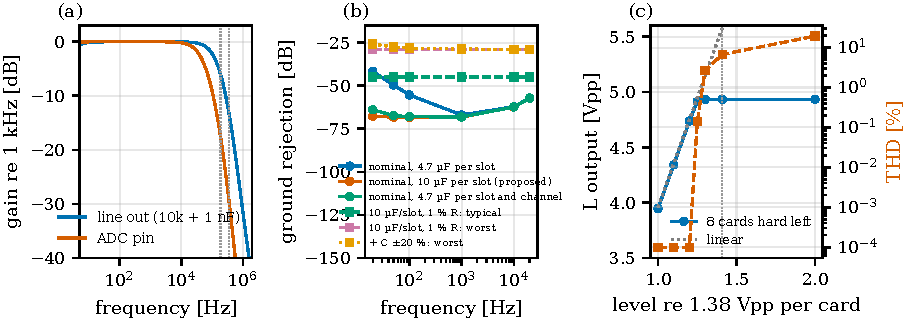
\includegraphics[width=\textwidth]{s12_mixer_2bus.pdf}
\caption{S12, two buses: (a) response to the line out and to the ADC pin; (b) ground rejection of the mirror
variants, nominal and with 1\,\% resistors and $\pm$20\,\% capacitors; (c) the L output with 8 hard-panned cards in
phase versus their level, and its THD.}\label{fig:s12}
\end{figure}

\paragraph{VREF from +3V3 with two RC stages.} Revision 0.2 of the backplane had its own CJ431 reference
(\SI{2.5}{V} from the \SI{5}{V}, \SI{10}{k\ohm} / \SI{10}{\micro F}) and an MCP6002 follower. In 0.3 VREF is a divider
from the controller's \SI{3.3}{V} LDO, \SI{10}{k\ohm} / \SI{27}{k\ohm} with \SI{10}{\micro F}, followed by a second
\SI{10}{k\ohm} / \SI{10}{\micro F} stage: \statStwelveVref\,V, corners at 2.2 and \SI{1.6}{Hz}, unbuffered. The
reasoning:
\begin{itemize}
  \item the summing amplifiers' + inputs are VREF's only DC load (picoamperes; the mirror network is AC coupled), so no
    buffer is needed;
  \item VREF reaches the line out about 1:1 (divided by 3.9 through $R_F'$, then the noise gain of 3.9), so its
    noise and ripple matter;
  \item the LDO rejects low-frequency ripple of the \SI{5}{V}; the two RC stages take out the MCU's own load steps on
    +3V3 (USB frames and the SYNC tick at \SI{1}{kHz}, the activity LED);
  \item the ADC tap's DC then follows the ADC's own \SI{3.3}{V} reference.
\end{itemize}
S12 compared the variants (Table~\ref{tab:vref}, Figure~\ref{fig:vref}). Two stages give \SI{-72}{dB} at \SI{100}{Hz}
and \SI{-112}{dB} at \SI{1}{kHz} from +3V3 to the line out, against \SI{-36}{dB} / \SI{-56}{dB} with one stage. From
the \SI{5}{V} rail, all three variants reach \SIrange{-69}{-73}{dB}; the reference without the CJ431 is
slightly better, because the CJ431's own supply rejection no longer enters. At a \SI{4.6}{V} supply all three
variants keep 8 hard-panned cards undistorted at the capped level. The CJ431, its feed resistor and the follower
are saved.

\begin{table}[htbp]
\centering\small
\caption{S12: the mixer's reference variants (\file{docs/results/s12\_mixer\_2bus.csv}); generated. Ripple
transfer to the line out in dB; ``--'': not applicable.}\label{tab:vref}
% generated by gen_tables.py -- do not edit
\begin{tabular}{@{}l r r r@{}}
\toprule
Reference & \shortstack[r]{+3V3, two\\RC stages\\(built)} & \shortstack[r]{+3V3, one\\RC stage} & \shortstack[r]{CJ431 +\\follower\\(rev 0.2)} \\
\midrule
VREF & 2.41\,V & 2.41\,V & 2.50\,V \\
ADC tap, DC & 1.55\,V & 1.55\,V & 1.61\,V \\
+3V3 ripple $\to$ line out, 20\,Hz & $-$45\,dB & $-$22\,dB & -- \\
\quad 100\,Hz & $-$72\,dB & $-$36\,dB & -- \\
\quad 1\,kHz & $-$112\,dB & $-$56\,dB & -- \\
\quad 10\,kHz & $-$152\,dB & $-$76\,dB & -- \\
5\,V ripple $\to$ line out, 100\,Hz & $-$73\,dB & $-$73\,dB & $-$71\,dB \\
\quad 1\,kHz & $-$71\,dB & $-$71\,dB & $-$69\,dB \\
\quad 10\,kHz & $-$71\,dB & $-$71\,dB & $-$69\,dB \\
Output noise, 8 slots & 17.0\,\textmu V & 17.0\,\textmu V & 17.5\,\textmu V \\
THD at 4.6\,V, 8 cards at 1.0 / 1.2$\times$ & $<$0.01 / 4.5\,\% & $<$0.01 / 4.5\,\% & $<$0.01 / 5.9\,\% \\
\bottomrule
\end{tabular}

\end{table}

\begin{figure}[htbp]
\centering
% generated by gen_tables.py -- do not edit
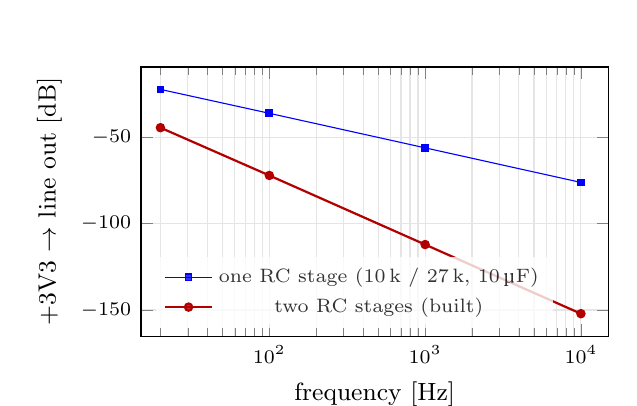
\begin{tikzpicture}
\begin{semilogxaxis}[width=0.62\textwidth,height=5.0cm,xlabel={frequency [Hz]},ylabel={+3V3 $\to$ line out [dB]},grid=both,grid style={black!10},xmin=15,xmax=15000,legend pos=south west,legend style={font=\scriptsize,draw=none,fill=white,fill opacity=0.8},tick label style={font=\scriptsize},label style={font=\small}]
\addplot[blue,mark=square*,mark size=1.2pt] coordinates {(20,-22.3609) (100,-36.1908) (1000,-56.1846) (10000,-76.1926)}; \addlegendentry{one RC stage (10\,k / 27\,k, 10\,\textmu F)}
\addplot[red!70!black,thick,mark=*,mark size=1.3pt] coordinates {(20,-44.5064) (100,-72.1612) (1000,-112.148) (10000,-152.156)}; \addlegendentry{two RC stages (built)}
\end{semilogxaxis}
\end{tikzpicture}

\caption{Ripple on +3V3 at the line out for one and two RC stages in the VREF divider (generated from
\file{docs/results/s12\_mixer\_2bus.csv}).}\label{fig:vref}
\end{figure}

\subsection{Effects slot}\label{sec:fxslot}
Slot~1 can hold an effects card (reverb and similar; a separate future board in the card format, for example a
CH32V307 with an ES8388 codec) instead of a voice. A reverb cannot run on a card (\SI{8}{KB} of RAM) or on the
controller, and there is no room for an extra header, so the slot is made convertible
(\file{docs/backplane.md} 5.1). Pins 15 and 14 of slot~1 carry CLK and SWIO\_1 through \SI{0}{\ohm} (R79, R81,
fitted) or the stereo mix through \SI{220}{\ohm} (R80, R82, not fitted): converting means swapping those four
0603 parts. Slot~1's pins 3 and 4, GND on every other slot, carry the effects card's loop-through return; a voice
card grounds them harmlessly, since they only reach two not-fitted \SI{220}{\ohm} positions (R83, R84) into the
line-out stage, and slot~1 keeps GND on pins 8, 13 and 16. The card has everything else in the slot: +5\,V, BCAST and SYNC for control and tempo, NRST, and its
audio pins into the mixer. Two uses, chosen in the effects card's firmware:
\begin{itemize}
  \item \textbf{mixing in:} the effect returns through the slot's audio pins like a voice. The send then contains the
    return (one summing stage), so the card keeps the loop gain (mixer $0.357\times$ wet level $\times$ its own
    gain) below about 0.5 without relying on any cancellation, may cancel its own return digitally (fixed codec
    delay), and limits the wet path;
  \item \textbf{loop-through:} the card mutes its audio pins and drives dry plus effect on pins 3 and 4, which then
    feed the line-out stage instead of the mixer (R83, R84 fitted; the line-out \SI{220}{\ohm} R71, R75 removed).
    There is no loop at all, and the instrument keeps its one line out.
\end{itemize}
With an effects card fitted the instrument has at most 7 voices; the controller finds it by enumeration (a
capability bit in HELLO) and maps MIDI CC~91 (reverb level) to it.

\subsection{Mechanics and floorplan}
\begin{itemize}
  \item \textbf{Slots:} slot $k$ has its socket centre at $x_k = 20 + 10(k-1)$\,mm along the south part of the board.
    The cards stand over the slot row and cover \SI{50}{mm} of its depth; the controller strip of about \SI{42}{mm}
    along the rear edge stays uncovered.
  \item \textbf{Orientation:} socket pin~1 is at the south-west corner of each socket; the cards' part side faces west
    (toward slot~1 and the mixer). The supply and audio end of every socket faces away from the controller strip, the
    bus end towards it. The card-plane offset from the socket centre line (about \SI{3.3}{mm}) assumes standard
    right-angle header geometry and is still to be checked with the chosen parts.
  \item \textbf{Card guides:} two 3D-printed slotted rails along the slot row, at the cards' side edges. The grooves
    sit at the card plane, so a card turned by \SI{180}{\degree} does not enter them. For the first build the headers
    alone hold the cards; four M3 holes are provided.
  \item \textbf{Zones:} analog in the west (mixer common block, line-out jack on the west edge), USB and power in the
    east, the MCU in between. The USB-A and USB-C receptacles and the SWD header sit on the rear edge, the power entry
    (JP1, J4) on the east edge. The summing nodes run along the slot row as a band on the bottom layer, the L$-$/L+ and R+/R$-$ tracks
    side by side so that pickup is common to both inputs, with guard tracks.
\end{itemize}
Figure~\ref{fig:floorbp} is drawn from the placement script; it shows the placement regions and anchored parts as
they stand when this report is built.

\begin{figure}[htbp]
\centering
% generated by gen_tables.py -- do not edit
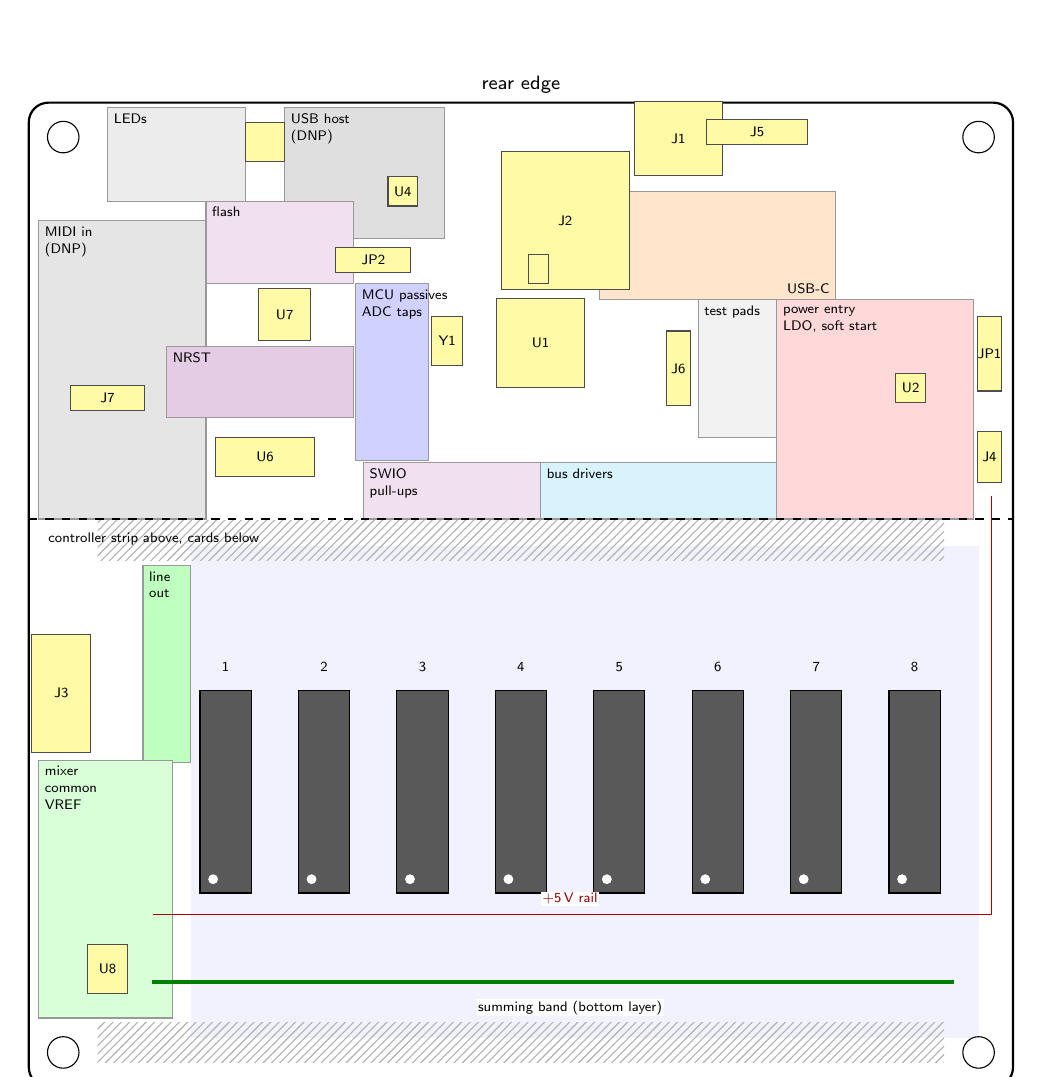
\begin{tikzpicture}[x=0.125cm,y=-0.125cm,font=\scriptsize\sffamily]
\draw[thick,rounded corners=0.25cm] (0,0) rectangle (100,100);
\fill[blue!5] (16.5,45) rectangle (96.5,95);
\fill[pattern=north east lines,pattern color=black!30] (7,42.5) rectangle (93,46.5);
\fill[pattern=north east lines,pattern color=black!30] (7,93.5) rectangle (93,97.5);
\filldraw[fill=gray!15,draw=black!40] (8,0.5) rectangle (22,10);
\node[align=left,anchor=north west,inner sep=1pt,font=\tiny\sffamily] at (8.3,0.8) {LEDs};
\filldraw[fill=gray!25,draw=black!40] (26,0.5) rectangle (42.2,13.8);
\node[align=left,anchor=north west,inner sep=1pt,font=\tiny\sffamily] at (26.3,0.8) {USB host\\(DNP)};
\filldraw[fill=gray!20,draw=black!40] (1,12) rectangle (18,42.3);
\node[align=left,anchor=north west,inner sep=1pt,font=\tiny\sffamily] at (1.3,12.3) {MIDI in\\(DNP)};
\filldraw[fill=violet!12,draw=black!40] (18,10) rectangle (33,18.4);
\node[align=left,anchor=north west,inner sep=1pt,font=\tiny\sffamily] at (18.3,10.3) {flash};
\filldraw[fill=violet!20,draw=black!40] (14,24.8) rectangle (33,32);
\node[align=left,anchor=north west,inner sep=1pt,font=\tiny\sffamily] at (14.3,25.1) {NRST};
\filldraw[fill=blue!18,draw=black!40] (33.2,18.4) rectangle (40.6,36.4);
\node[align=left,anchor=north west,inner sep=1pt,font=\tiny\sffamily] at (33.5,18.7) {MCU passives\\ADC taps};
\filldraw[fill=violet!12,draw=black!40] (34,36.6) rectangle (52,42.3);
\node[align=left,anchor=north west,inner sep=1pt,font=\tiny\sffamily] at (34.3,36.9) {SWIO\\pull-ups};
\filldraw[fill=cyan!15,draw=black!40] (52,36.6) rectangle (76,42.3);
\node[align=left,anchor=north west,inner sep=1pt,font=\tiny\sffamily] at (52.3,36.9) {bus drivers};
\filldraw[fill=gray!10,draw=black!40] (68,20) rectangle (76,34);
\node[align=left,anchor=north west,inner sep=1pt,font=\tiny\sffamily] at (68.3,20.3) {test pads};
\filldraw[fill=orange!20,draw=black!40] (58,9) rectangle (82,20);
\node[align=right,anchor=south east,inner sep=1pt,font=\tiny\sffamily] at (81.7,19.7) {USB-C};
\filldraw[fill=red!15,draw=black!40] (76,20) rectangle (96,42.3);
\node[align=left,anchor=north west,inner sep=1pt,font=\tiny\sffamily] at (76.3,20.3) {power entry\\LDO, soft start};
\filldraw[fill=green!25,draw=black!40] (11.6,47) rectangle (16.4,67);
\node[align=left,anchor=north west,inner sep=1pt,font=\tiny\sffamily] at (11.9,47.3) {line\\out};
\filldraw[fill=green!15,draw=black!40] (1,66.8) rectangle (14.6,93);
\node[align=left,anchor=north west,inner sep=1pt,font=\tiny\sffamily] at (1.3,67.1) {mixer\\common\\VREF};
\filldraw[fill=yellow!35,draw=black!70] (47.5,19.9) rectangle (56.5,28.9);
\node[align=center,font=\tiny\sffamily,inner sep=0pt] at (52,24.4) {U1};
\filldraw[fill=yellow!35,draw=black!70] (19,34) rectangle (29,38);
\node[align=center,font=\tiny\sffamily,inner sep=0pt] at (24,36) {U6};
\filldraw[fill=yellow!35,draw=black!70] (23.35,18.85) rectangle (28.65,24.15);
\node[align=center,font=\tiny\sffamily,inner sep=0pt] at (26,21.5) {U7};
\filldraw[fill=yellow!35,draw=black!70] (6,85.5) rectangle (10,90.5);
\node[align=center,font=\tiny\sffamily,inner sep=0pt] at (8,88) {U8};
\filldraw[fill=yellow!35,draw=black!70] (61.5,-0.075) rectangle (70.5,7.425);
\node[align=center,font=\tiny\sffamily,inner sep=0pt] at (66,3.675) {J1};
\filldraw[fill=yellow!35,draw=black!70] (48,5) rectangle (61,19);
\node[align=center,font=\tiny\sffamily,inner sep=0pt] at (54.5,12) {J2};
\filldraw[fill=yellow!35,draw=black!70] (0.3,54) rectangle (6.3,66);
\node[align=center,font=\tiny\sffamily,inner sep=0pt] at (3.3,60) {J3};
\filldraw[fill=yellow!35,draw=black!70] (68.9,1.75) rectangle (79.1,4.25);
\node[align=center,font=\tiny\sffamily,inner sep=0pt] at (74,3) {J5};
\filldraw[fill=yellow!35,draw=black!70] (96.35,33.45) rectangle (98.85,38.55);
\node[align=center,font=\tiny\sffamily,inner sep=0pt] at (97.6,36) {J4};
\filldraw[fill=yellow!35,draw=black!70] (96.35,21.7) rectangle (98.85,29.3);
\node[align=center,font=\tiny\sffamily,inner sep=0pt] at (97.6,25.5) {JP1};
\filldraw[fill=yellow!35,draw=black!70] (64.75,23.2) rectangle (67.25,30.8);
\node[align=center,font=\tiny\sffamily,inner sep=0pt] at (66,27) {J6};
\filldraw[fill=yellow!35,draw=black!70] (4.2,28.75) rectangle (11.8,31.25);
\node[align=center,font=\tiny\sffamily,inner sep=0pt] at (8,30) {J7};
\filldraw[fill=yellow!35,draw=black!70] (31.2,14.75) rectangle (38.8,17.25);
\node[align=center,font=\tiny\sffamily,inner sep=0pt] at (35,16) {JP2};
\filldraw[fill=yellow!35,draw=black!70] (40.9,21.7) rectangle (44.1,26.7);
\node[align=center,font=\tiny\sffamily,inner sep=0pt] at (42.5,24.2) {Y1};
\filldraw[fill=yellow!35,draw=black!70] (88.1,27.5) rectangle (91.1,30.5);
\node[align=center,font=\tiny\sffamily,inner sep=0pt] at (89.6,29) {U2};
\filldraw[fill=yellow!35,draw=black!70] (22,2) rectangle (26,6);
\filldraw[fill=yellow!35,draw=black!70] (36.5,7.5) rectangle (39.5,10.5);
\node[align=center,font=\tiny\sffamily,inner sep=0pt] at (38,9) {U4};
\filldraw[fill=yellow!35,draw=black!70] (50.8,15.4) rectangle (52.8,18.4);
\filldraw[fill=black!65,draw=black] (17.4,59.72) rectangle (22.6,80.3);
\node[font=\tiny\sffamily] at (20,57.32) {1};
\fill[white] (18.73,78.9) circle (0.5);
\filldraw[fill=black!65,draw=black] (27.4,59.72) rectangle (32.6,80.3);
\node[font=\tiny\sffamily] at (30,57.32) {2};
\fill[white] (28.73,78.9) circle (0.5);
\filldraw[fill=black!65,draw=black] (37.4,59.72) rectangle (42.6,80.3);
\node[font=\tiny\sffamily] at (40,57.32) {3};
\fill[white] (38.73,78.9) circle (0.5);
\filldraw[fill=black!65,draw=black] (47.4,59.72) rectangle (52.6,80.3);
\node[font=\tiny\sffamily] at (50,57.32) {4};
\fill[white] (48.73,78.9) circle (0.5);
\filldraw[fill=black!65,draw=black] (57.4,59.72) rectangle (62.6,80.3);
\node[font=\tiny\sffamily] at (60,57.32) {5};
\fill[white] (58.73,78.9) circle (0.5);
\filldraw[fill=black!65,draw=black] (67.4,59.72) rectangle (72.6,80.3);
\node[font=\tiny\sffamily] at (70,57.32) {6};
\fill[white] (68.73,78.9) circle (0.5);
\filldraw[fill=black!65,draw=black] (77.4,59.72) rectangle (82.6,80.3);
\node[font=\tiny\sffamily] at (80,57.32) {7};
\fill[white] (78.73,78.9) circle (0.5);
\filldraw[fill=black!65,draw=black] (87.4,59.72) rectangle (92.6,80.3);
\node[font=\tiny\sffamily] at (90,57.32) {8};
\fill[white] (88.73,78.9) circle (0.5);
\draw[red!70!black,line width=0.6pt] (97.8,40) -- (97.8,82.5) -- (12.6,82.5);
\draw[green!50!black,line width=1.2pt] (12.5,89.35) -- (94,89.35);
\node[font=\tiny\sffamily,fill=white,inner sep=0.5pt] at (55,91.95) {summing band (bottom layer)};
\node[font=\tiny\sffamily,red!60!black,fill=white,inner sep=0.5pt] at (55,80.9) {+5\,V rail};
\draw (3.5,3.5) circle (1.6);
\draw (96.5,3.5) circle (1.6);
\draw (3.5,96.5) circle (1.6);
\draw (96.5,96.5) circle (1.6);
\draw[dashed] (0,42.3) -- (100,42.3);
\node[anchor=west,font=\tiny\sffamily] at (1,44.3) {controller strip above, cards below};
\node[anchor=south,font=\scriptsize\sffamily] at (50,0) {rear edge};
\end{tikzpicture}

\caption{Backplane floorplan (KiCad orientation: rear edge at the top), generated from \file{hw/pcb\_place\_bp.py}:
placement regions, anchored ICs and connectors (yellow), the 8 slot sockets (pin~1 marked), card area (light blue),
card-guide bands (hatched), the +5\,V trunk and rail and the summing band.}
\label{fig:floorbp}
\end{figure}

\subsection{PCB}
The backplane is a 4-layer board of 100\,$\times$\,100\,mm (JLCPCB, \SI{1.6}{mm}). It was planned as a 2-layer
board; routed on two layers, the area around the MCU left a few nets open in every run (+3V3 to the VDD pins, the
SPI and SWD lines) and the bottom pour broke into islands there, so the stack became:
\begin{itemize}
  \item \textbf{F.Cu:} all parts and most signals; ground fill in the free areas.
  \item \textbf{In1:} GND, solid over the whole board.
  \item \textbf{In2:} +3V3 under the controller strip, GND under the slot area, so the summing band on B.Cu sits
    directly against ground.
  \item \textbf{B.Cu:} signals and the summing band; ground fill. +5\,V stays on its pre-routed trunk and rail
    (110\,mA).
\end{itemize}
The other layout rules of \file{docs/backplane.md}~7 carry over:
\begin{itemize}
  \item \textbf{Bus in the socket field:} each bus track runs in its own gap between socket pin positions (SYNC 4|5,
    BCAST 5|6, RETURN 6|7, CLK 7|8), so each reaches its pin with a short jog and no crossing.
  \item \textbf{Separation:} the analog zone (mixer, line out, summing band) in the west and south; the USB ports, the
    power entry and the LDO in the north and east; the MCU in the middle of the controller strip with a free fan-out
    zone around it.
  \item \textbf{Placement by function:} one region per function (power, USB, SPI flash and 595, ADC dividers, bus
    resistors, SWIO pull-ups, MIDI option), explicit anchors for connectors, ICs and decoupling. The flash and the 595
    sit together west of the MCU, the crystal at its west pins, the UART header east of it.
  \item \textbf{Scripted placement and pre-routes} (\file{hw/pcb\_place\_bp.py}, \file{hw/gen\_pcb\_bp.py}): the
    \SI{5}{V} trunk and rail, the bus tracks in the socket field, the per-slot audio fan-out and the summing band are
    laid before Freerouting runs; GND connects through the planes and stitching vias.
\end{itemize}
\textbf{Result:} \statBpSegments{} track segments, \statBpLenF{}\,m on F.Cu and \statBpLenB{}\,m on B.Cu, \statBpVias{} vias
(\statBpGndVias{} of them GND); DRC with schematic parity: 0 violations, 0 unconnected pads, no isolated copper. As a check, the same placement routed on two layers (\texttt{BP\_LAYERS=2}) leaves a
single connection open (+3V3 at one MCU supply pin) with 7\,\% more track: the placement is sound, and the four
layers buy solid planes, short return paths and a ground reference for the summing band.
Figures~\ref{fig:bplayers} and~\ref{fig:bprender} show the board as generated by \file{hw/pcb\_figures.py}.

\begin{figure}[p]
\centering
\begin{subfigure}{0.43\textwidth}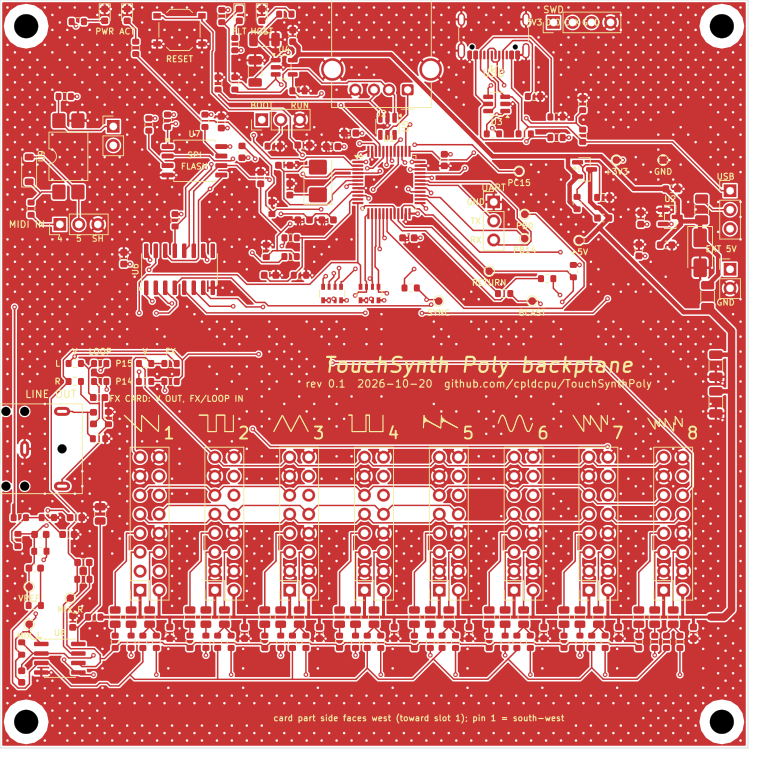
\includegraphics[width=\linewidth]{backplane_pcb/top.png}\caption{F.Cu with silkscreen}\end{subfigure}\hfill
\begin{subfigure}{0.43\textwidth}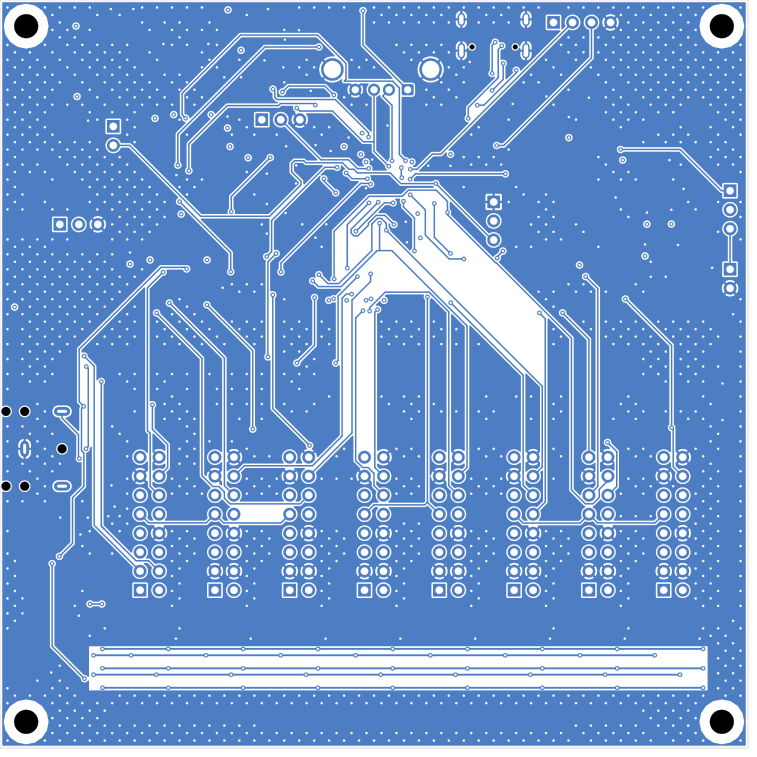
\includegraphics[width=\linewidth]{backplane_pcb/bcu.png}\caption{B.Cu}\end{subfigure}\\[6pt]
\begin{subfigure}{0.43\textwidth}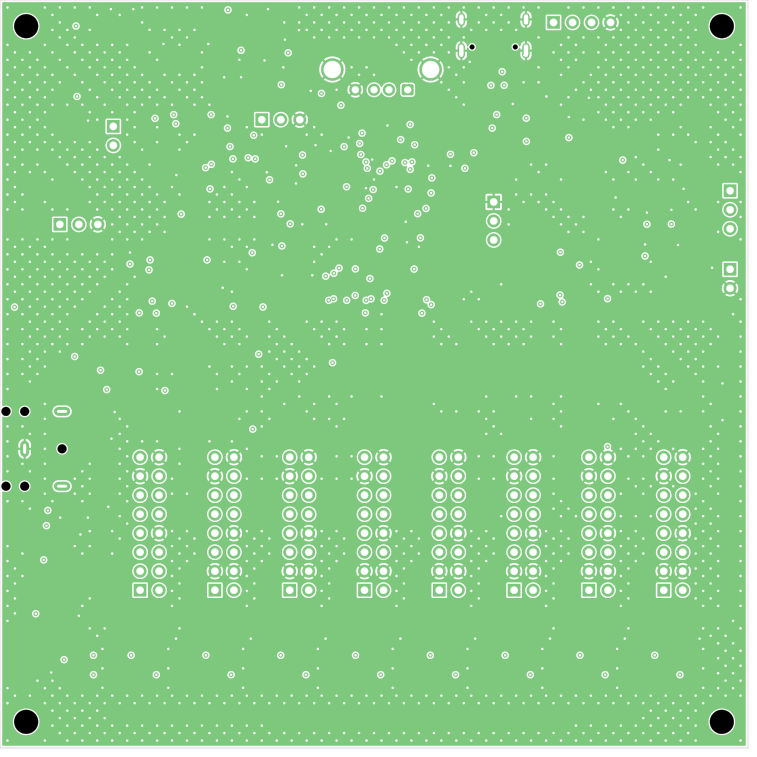
\includegraphics[width=\linewidth]{backplane_pcb/in1.png}\caption{In1: GND}\end{subfigure}\hfill
\begin{subfigure}{0.43\textwidth}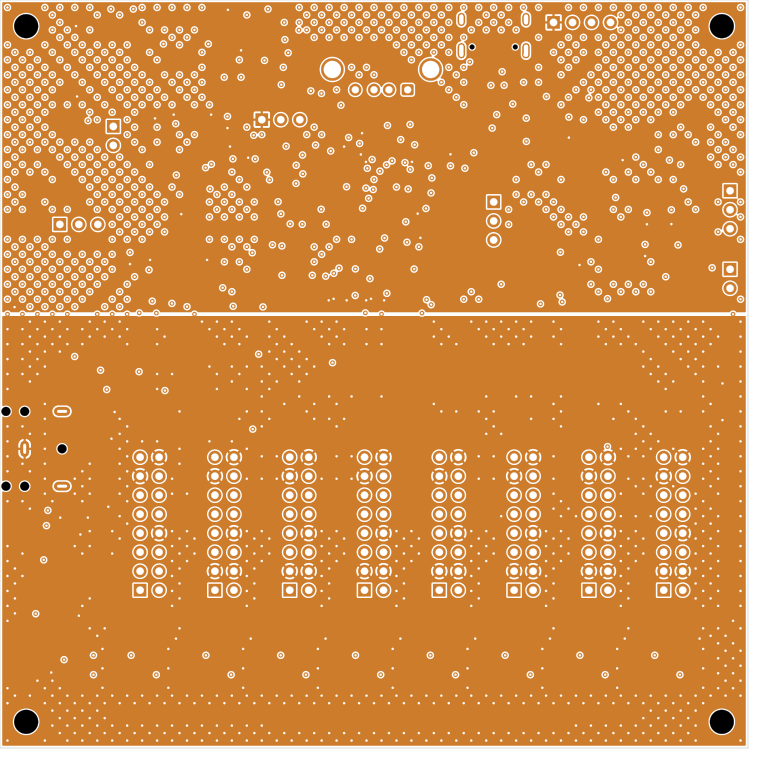
\includegraphics[width=\linewidth]{backplane_pcb/in2.png}\caption{In2: +3V3 (strip), GND (slots)}\end{subfigure}\\[6pt]
\begin{subfigure}{0.43\textwidth}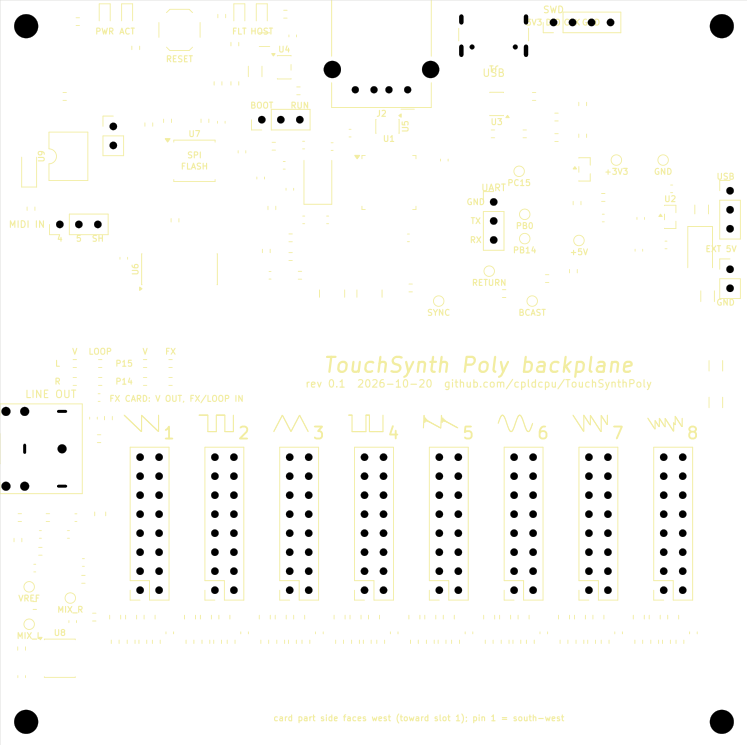
\includegraphics[width=\linewidth]{backplane_pcb/silk.png}\caption{top silkscreen}\end{subfigure}\hfill
\begin{subfigure}{0.43\textwidth}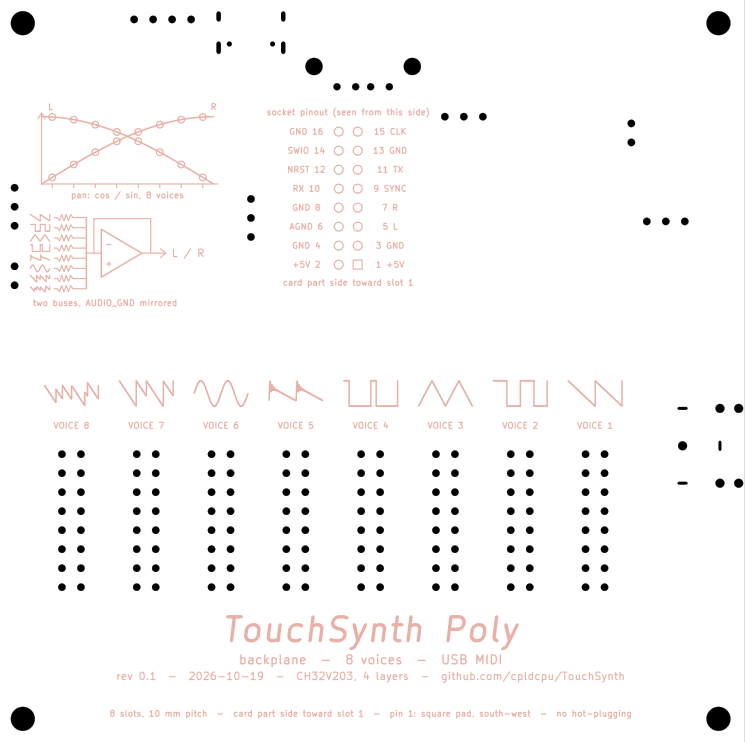
\includegraphics[width=\linewidth]{backplane_pcb/bsilk.png}\caption{bottom silkscreen (seen from the back)}\end{subfigure}
\caption{Backplane layers, seen from the top unless noted (\file{docs/figures/backplane\_pcb/}, generated by
\file{hw/pcb\_figures.py}).}\label{fig:bplayers}
\end{figure}

\begin{figure}[p]
\centering
\begin{subfigure}{0.64\textwidth}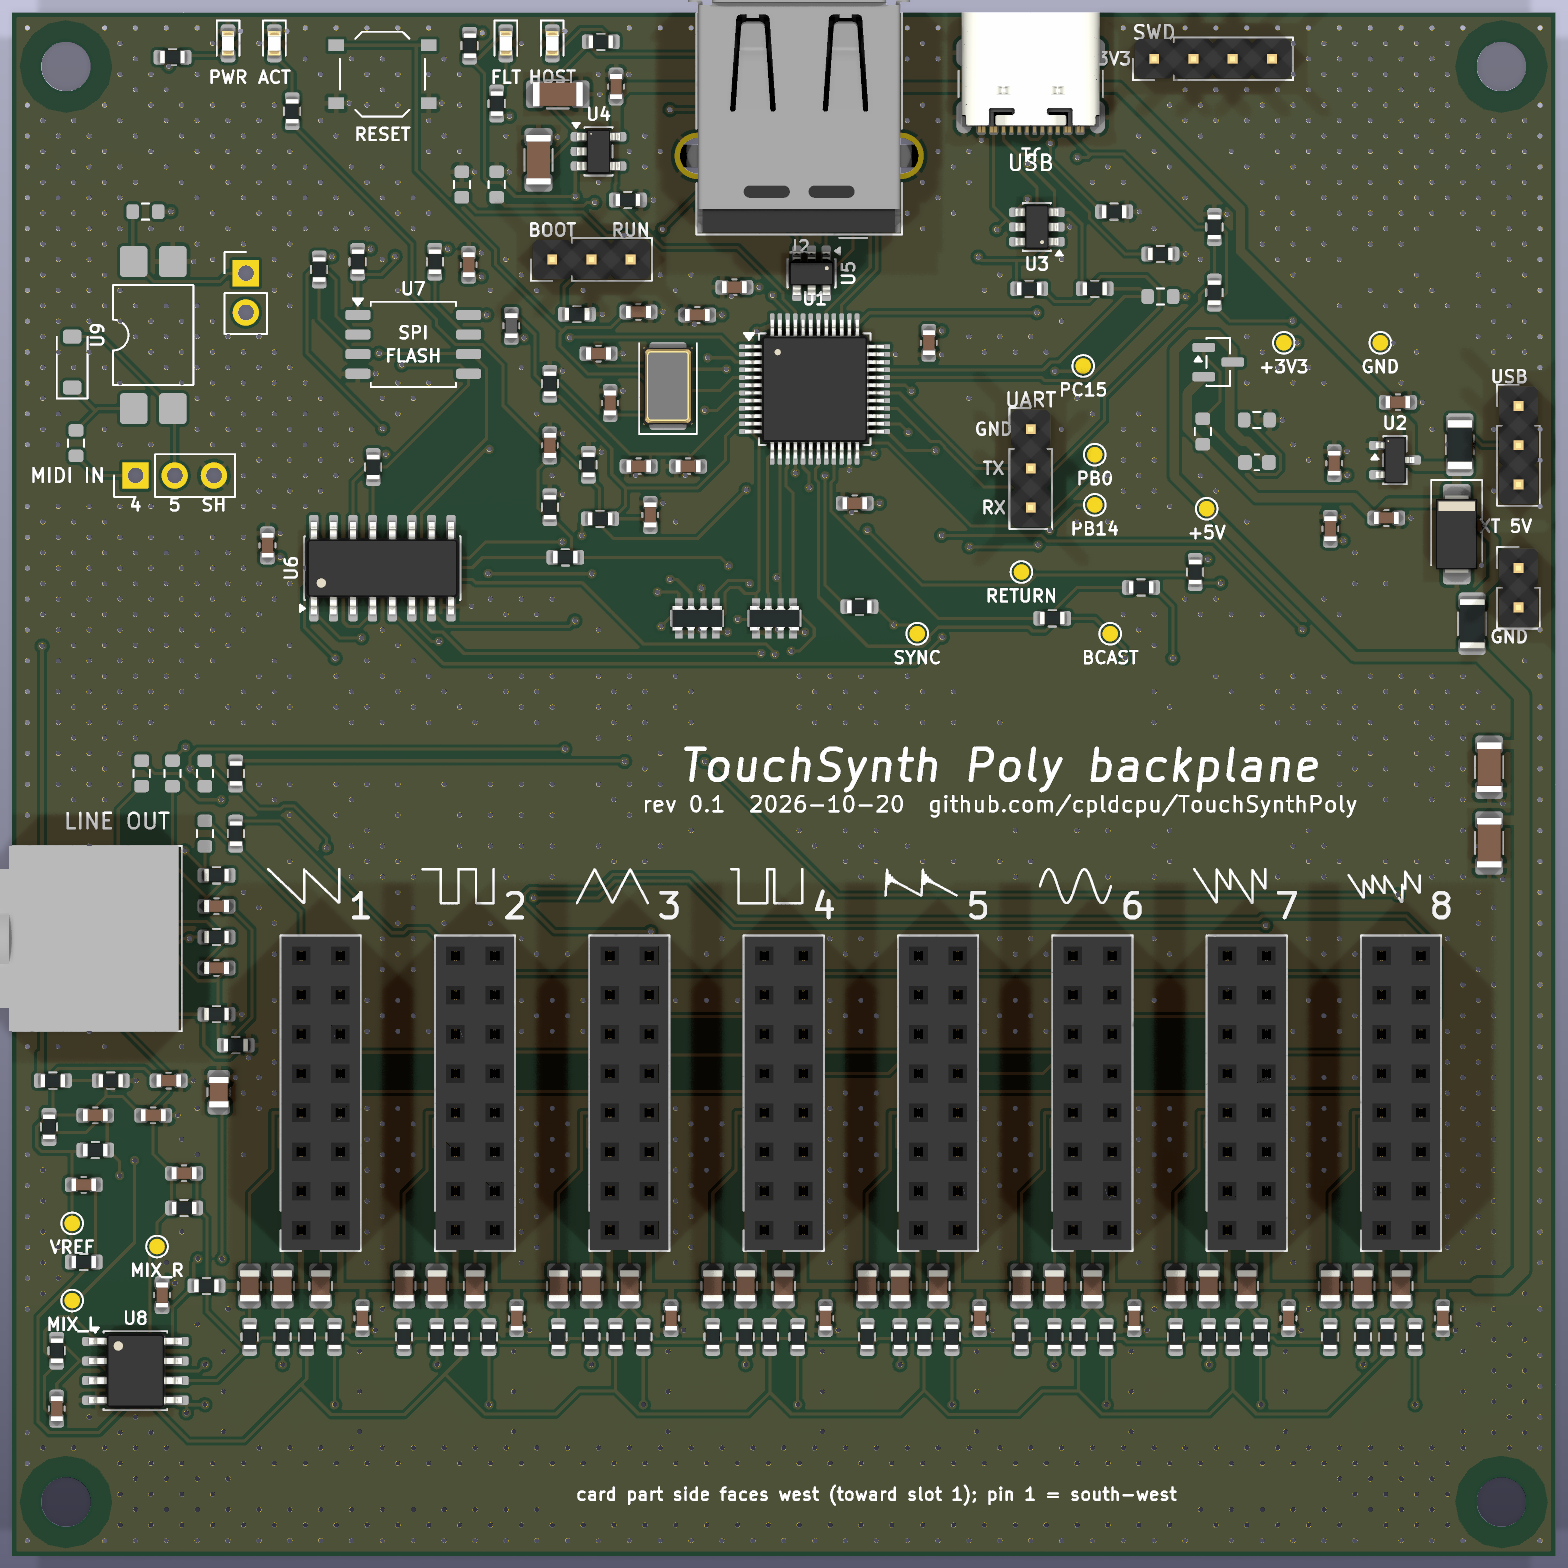
\includegraphics[width=\linewidth]{backplane_pcb/render_top.png}\caption{top}\end{subfigure}\\[6pt]
\begin{subfigure}{0.64\textwidth}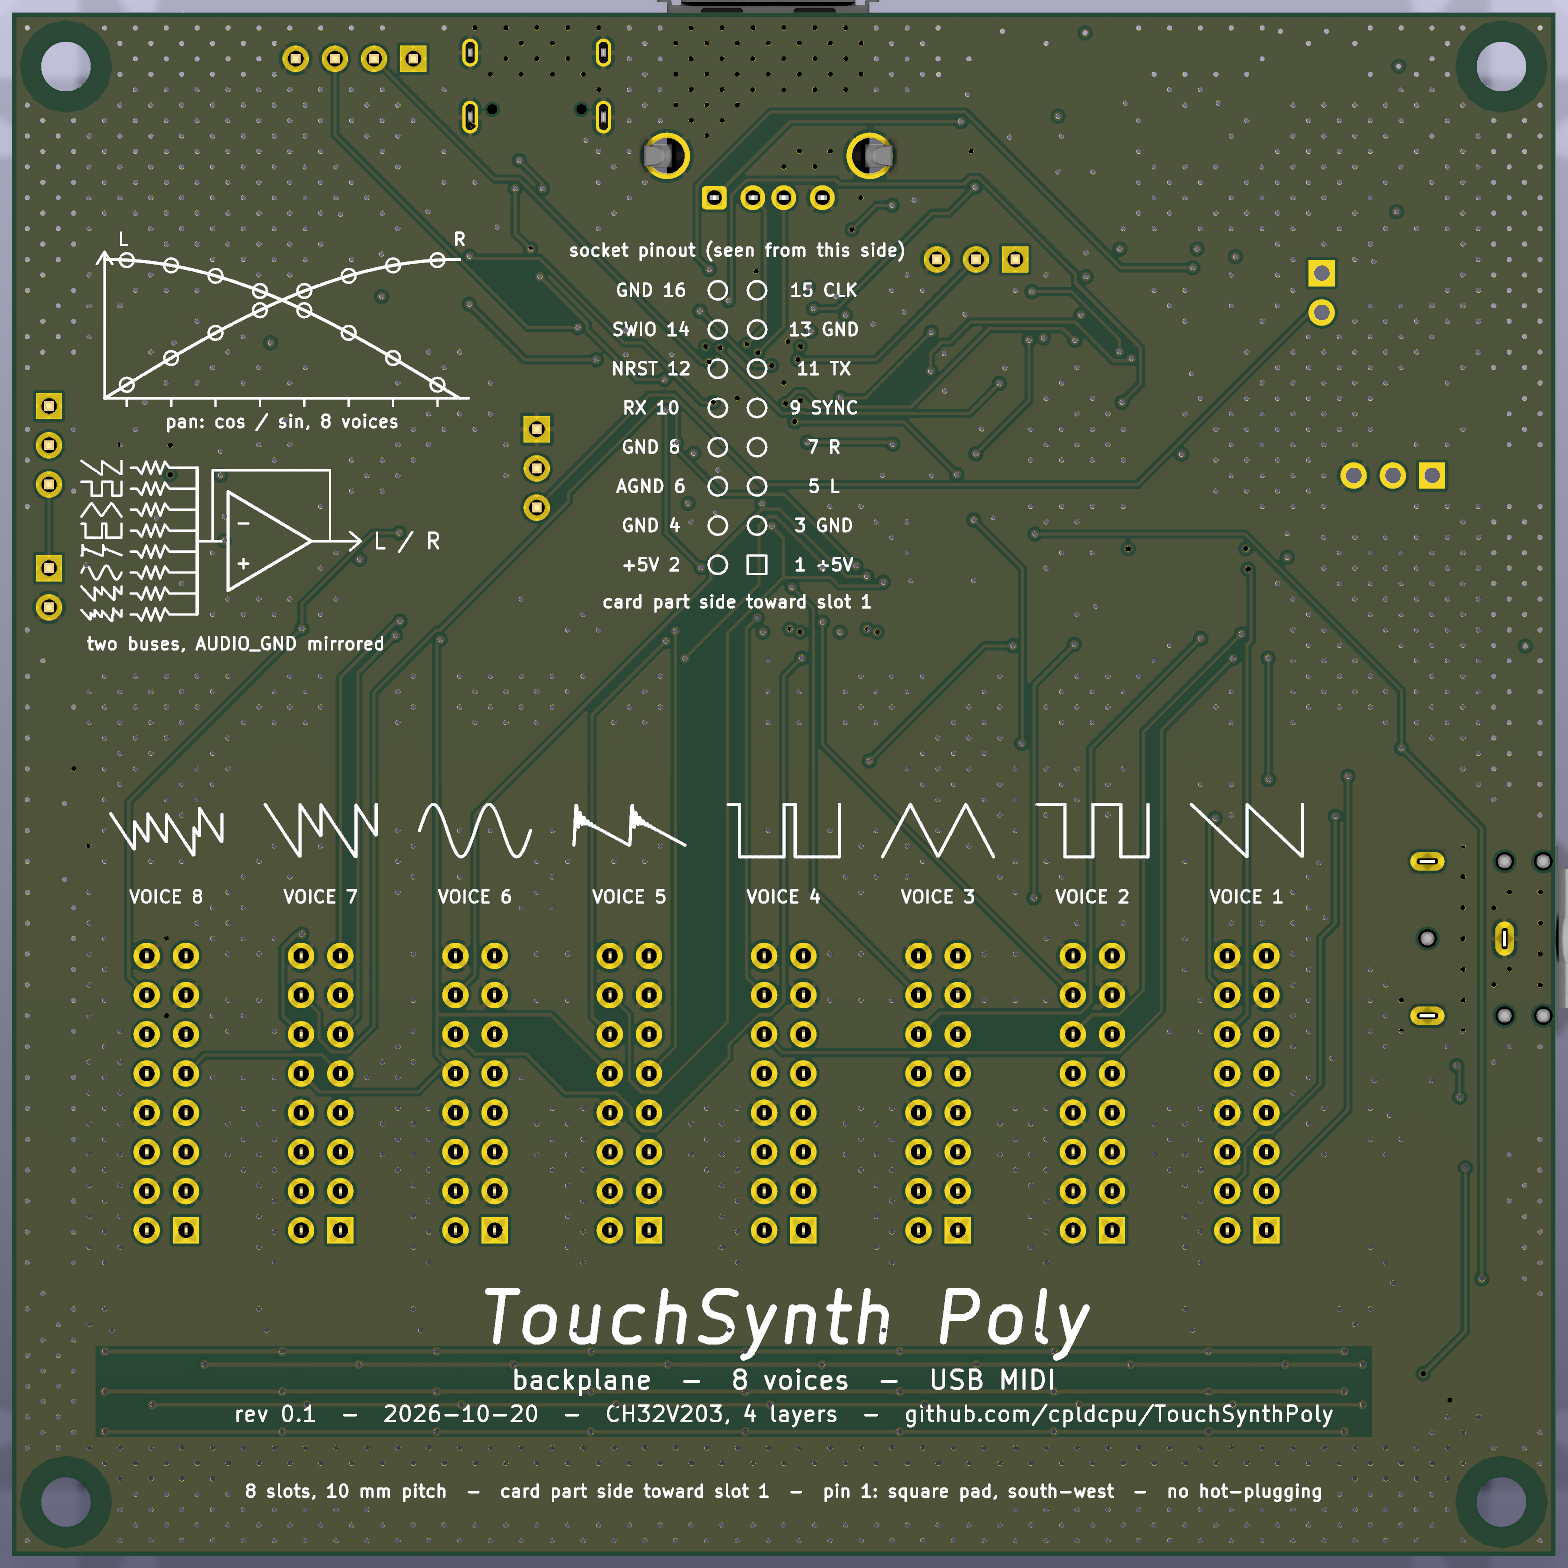
\includegraphics[width=\linewidth]{backplane_pcb/render_bottom.png}\caption{bottom}\end{subfigure}
\caption{Backplane 3D renders (not-fitted parts left out).}\label{fig:bprender}
\end{figure}

% =====================================================================================================================
\section{Voice bus protocol}\label{sec:bus}
The protocol is specified in \file{docs/bus.md}. Its goals, in order:
\begin{enumerate}
  \item \textbf{Synchronisation first:} every card turns the same event into sound at the same moment, to within a few
    microseconds, independent of when the bytes reach it, how busy it is or where it is in its DAC buffer.
  \item \textbf{Fixed latency instead of minimal latency:} a constant delay of a few milliseconds is accepted; jitter
    between voices is not.
  \item \textbf{Simple and robust:} broadcast without acknowledgements; lost packets are repaired by periodic
    refreshes; one card talks at a time on the return line, and only when asked.
\end{enumerate}

\subsection{Physical layer}
\begin{table}[htbp]
\centering\small
\caption{Bus lines.}\label{tab:busphy}
\begin{tabularx}{\textwidth}{@{}l l X@{}}
\toprule
Line & Driver & Electrical \\
\midrule
BCAST (card RX) & controller USART3 TX, push-pull & \SI{1}{Mbaud} 8N1, \SI{33}{\ohm} series resistor at the controller,
  \SI{100}{\ohm} on the card \\
RETURN (card TX) & the addressed card only, open drain & \SI{1}{k\ohm} pull-up to \SI{3.3}{V} on the backplane \\
SYNC & controller TIM1 CH1, push-pull & \SI{1}{kHz} square; the rising edge starts a frame; \SI{100}{k\ohm} pull-down
  on the card (standalone detection) \\
NRST & 74HC595 output per slot, direct & reset and enumeration; no series resistor or pull-down \\
SWIO & controller GPIO per slot, open drain & programming (WCH one-wire debug protocol) \\
\bottomrule
\end{tabularx}
\end{table}
At \SI{1}{Mbaud} a card's USART divider is exactly 3.0 (\SI{48}{MHz}/16) and its fractional resolution cannot correct
the HSI. The baud accuracy therefore comes from the HSITRIM coarse trim: within $\pm$\SI{0.1}{\percent} of the crystal
plus about \SI{0.02}{\percent} of wander, far inside the UART's $\pm$\SI{2}{\percent}. A card does not listen to the
bus until it has trimmed.

\subsection{Frames, lead and presentation delay}
\begin{itemize}
  \item \textbf{Frame:} the \SI{1}{ms} between two rising SYNC edges, numbered by the controller with a 16-bit counter
    sent in the FRAME packet at the start of each frame. All timing in the protocol is in frames; USB-MIDI delivers
    events in \SI{1}{ms} USB frames without timestamps, so finer timestamps would gain nothing.
  \item \textbf{Bus lead $L$:} the controller stamps each timed event with its execution frame, $L = 2$ frames after
    the frame in which it arrived. The event is sent at the start of the next frame; the cards parse what arrived before
    a tick in that tick and run the events that are due.
  \item \textbf{Presentation delay $D$:} what tick $n$ computes appears at the outputs at frame $n + D$. The CVs go
    through a delay line of $D$ ticks. The oscillator state $V_n$ (pitch, gate, phase reset, staged drum strikes) is
    queued with its target time $b_n = t_n + D\,\bar P$ in SysTick cycles; SysTick and TIM2 both count HCLK, so the
    renderer knows which carrier period each ring entry is played in and splits its block at $b_n$: oscillators exact
    to one carrier period (\SI{5.3}{\micro s}), the modal engine to one \SI{64}{\micro s} sample.
  \item \textbf{Choice of $D$:} $D$ must cover the DAC's render lead (two buffer halves) plus the tick's run time.
    With 256-period buffer halves (\SI{1.37}{ms}) $D = 4$; the 1024-period halves of rev 0.1 would need $D = 12$.
    The short halves also free \SI{3}{KB} of RAM.
\end{itemize}
Figure~\ref{fig:timing} shows the resulting timeline. From an event's arrival at the controller to sound:
$L + D$ frames plus the fraction of the arrival frame, \SIrange{6}{7}{ms}, the same for every event and every voice.

\begin{figure}[htbp]
\centering
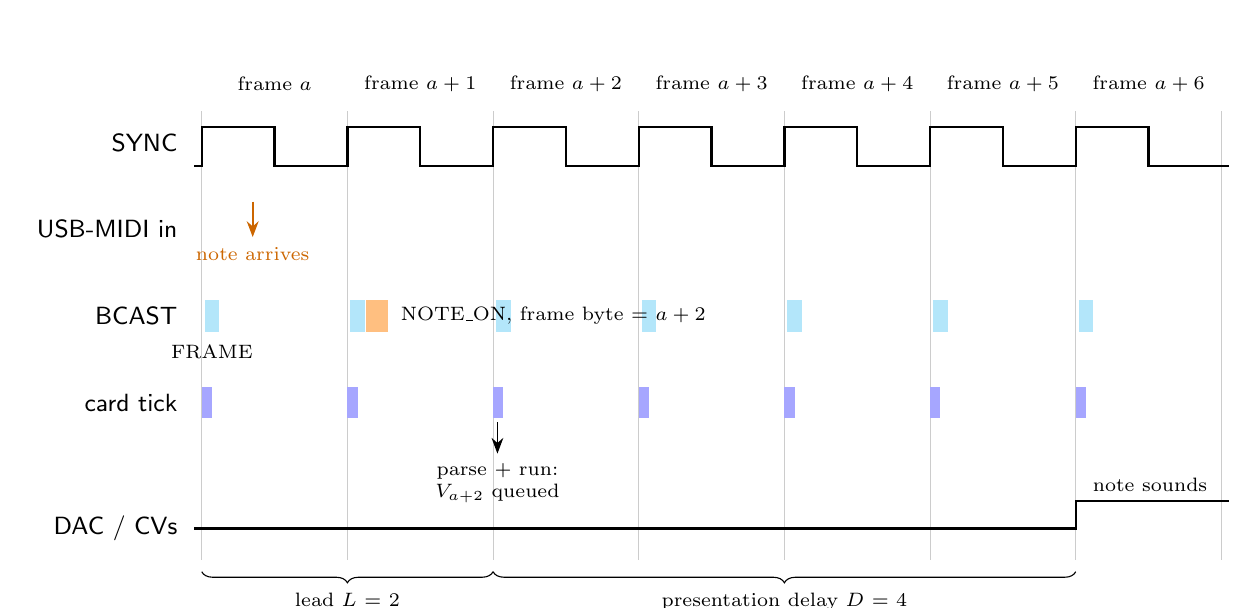
\begin{tikzpicture}[x=1.85cm, y=1cm, font=\small\sffamily, >={Stealth[length=2mm]}]
  % frame grid
  \foreach \i in {0,...,7} {
    \draw[black!20] (\i,0.4) -- (\i,-5.3);
  }
  \foreach \i/\l in {0/a, 1/a+1, 2/a+2, 3/a+3, 4/a+4, 5/a+5, 6/a+6} {
    \node[font=\scriptsize] at (\i+0.5,0.75) {frame $\l$};
  }
  % SYNC
  \node[anchor=east] at (-0.1,0) {SYNC};
  \draw[thick] (-0.05,-0.3) \foreach \i in {0,...,6} { -- (\i,-0.3) -- (\i,0.2) -- (\i+0.5,0.2) -- (\i+0.5,-0.3) } -- (7.05,-0.3);
  % MIDI arrival
  \node[anchor=east] at (-0.1,-1.1) {USB-MIDI in};
  \draw[->, thick, orange!80!black] (0.35,-0.75) -- (0.35,-1.2) node[below, font=\scriptsize]{note arrives};
  % BCAST
  \node[anchor=east] at (-0.1,-2.2) {BCAST};
  \foreach \i in {0,...,6} { \fill[cyan!30] (\i+0.02,-2.4) rectangle (\i+0.12,-2.0); }
  \fill[orange!50] (1.13,-2.4) rectangle (1.28,-2.0);
  \node[font=\scriptsize, align=left, anchor=west] at (1.3,-2.2) {NOTE\_ON, frame byte = $a+2$};
  \node[font=\scriptsize, anchor=north] at (0.07,-2.45) {FRAME};
  % card tick
  \node[anchor=east] at (-0.1,-3.3) {card tick};
  \foreach \i in {0,...,6} { \fill[blue!35] (\i,-3.5) rectangle (\i+0.07,-3.1); }
  \draw[->] (2.03,-3.55) -- (2.03,-3.95) node[below, font=\scriptsize, align=center]{parse + run:\\$V_{a+2}$ queued};
  % output
  \node[anchor=east] at (-0.1,-4.9) {DAC / CVs};
  \draw[thick] (-0.05,-4.9) -- (6.0,-4.9) -- (6.0,-4.55) -- (7.05,-4.55);
  \node[font=\scriptsize, anchor=west] at (6.05,-4.35) {note sounds};
  % braces
  \draw[decorate, decoration={brace, amplitude=4pt, mirror}] (0,-5.45) -- (2,-5.45) node[midway, below=4pt, font=\scriptsize]{lead $L$ = 2};
  \draw[decorate, decoration={brace, amplitude=4pt, mirror}] (2,-5.45) -- (6,-5.45) node[midway, below=4pt, font=\scriptsize]{presentation delay $D$ = 4};
\end{tikzpicture}
\caption{Timing of one note. An event arriving in frame $a$ is stamped for frame $a + L$, transmitted after FRAME at
the start of frame $a + 1$, parsed and executed by every card at the tick of frame $a + 2$, and appears at the DAC and
CV outputs at the SYNC edge of frame $a + L + D$, exact to one carrier period.}
\label{fig:timing}
\end{figure}

\paragraph{What limits the alignment.} The SYNC timestamp (EXTI entry, less than \SI{1}{\micro s} of jitter), the block
split (one carrier period) and the prediction of $b_n$ from $\bar P$ over $D$ frames (HSI wander of $2\times10^{-4}$
over 750 periods, a fraction of a period). Together a few microseconds.

\subsection{Framing: COBS and CRC-8}
Figure~\ref{fig:packet} shows the packet. Packets are COBS encoded and terminated by 0x00, so a receiver
resynchronises at the next zero byte after any error; a packet may also begin with 0x00 (the cards' replies do), and
empty packets are ignored. The decoded content is
\begin{itemize}
  \item controller $\to$ cards: \texttt{dst type [frame] payload crc8};
  \item card $\to$ controller: \texttt{src type payload crc8}.
\end{itemize}
\texttt{dst} is a voice bitmask (bit $k$ = the card with address $k$; 0xFF = all, including unaddressed cards;
0x00 = unaddressed cards, for enumeration). Timed messages carry the low 8 bits of the execution frame, read relative
to the card's counter: late events run at once and are counted, events more than 32 frames ahead are dropped. The
CRC is CRC-8 with polynomial 0x07, initial value 0, MSB first, no final XOR (CRC-8/SMBUS); the CRC over a whole packet
including its CRC byte is 0. Multi-byte values are little-endian; pitch is in 1/256 semitone. Unknown types are ignored.
Cards accept packets of up to 64 decoded bytes.

\begin{figure}[htbp]
\centering
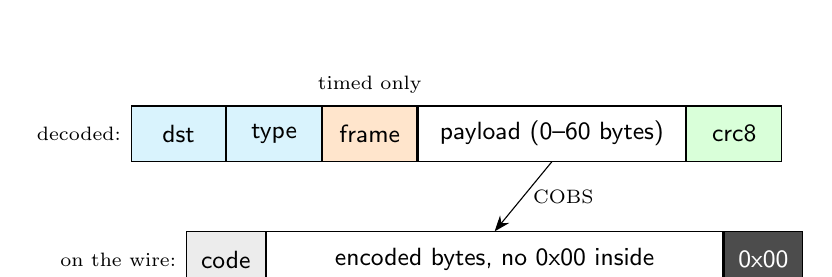
\begin{tikzpicture}[font=\small\sffamily, >={Stealth[length=2mm]},
  f/.style={draw, minimum height=7mm, minimum width=#1, inner sep=1pt, fill=white}, f/.default=12mm]
  \node[f, fill=cyan!15] (dst) at (0,0) {dst};
  \node[f, right=0pt of dst, fill=cyan!15] (type) {type};
  \node[f, right=0pt of type, fill=orange!20] (fr) {frame};
  \node[f=34mm, right=0pt of fr] (pay) {payload (0--60 bytes)};
  \node[f, right=0pt of pay, fill=green!15] (crc) {crc8};
  \node[anchor=east, font=\scriptsize] at (dst.west) {decoded:\ };
  \node[above=1pt of fr, font=\scriptsize] {timed only};
  \node[f=10mm, fill=gray!15] (code) at (0.6,-1.6) {code};
  \node[f=58mm, right=0pt of code] (enc) {encoded bytes, no 0x00 inside};
  \node[f=10mm, right=0pt of enc, fill=black!70, text=white] (del) {0x00};
  \node[anchor=east, font=\scriptsize] at (code.west) {on the wire:\ };
  \draw[->] ($(pay.south)+(0,0)$) -- node[right, font=\scriptsize]{COBS} ($(enc.north)+(0,0)$);
\end{tikzpicture}
\caption{Packet structure. CRC-8 covers dst to the last payload byte; COBS replaces every zero byte and adds one code
byte per 254 bytes; the 0x00 delimiter ends the packet.}
\label{fig:packet}
\end{figure}

\subsection{Messages}
Table~\ref{tab:msgs} lists the messages. Replies (HELLO, STATUS, CAL\_DATA, COUNTERS) are sent only in answer to a
REQUEST or ASSIGN. Only one request is outstanding at a time; the card answers within 2 frames and the controller
times out after 5. The chip ID in HELLO (the V006's 64-bit unique ID from its electronic signature) lets the controller
keep each card's calibration and identity even if cards change slots.

\begin{table}[htbp]
\centering\small
\caption{Bus messages (\file{docs/bus.md} 5).}\label{tab:msgs}
\begin{tabularx}{\textwidth}{@{}l l c >{\raggedright}p{4.2cm} >{\raggedright\arraybackslash}X@{}}
\toprule
Type & Name & Timed & Payload & Use \\
\midrule
0x01 & FRAME & & frame u16 & first packet of every frame; the cards check their counter \\
0x02 & CONFIG & & $D$, $L$, tuning i16, flags & system settings \\
0x03 & ASSIGN & & address & to dst 0x00: the released card takes the address and answers HELLO \\
0x10 & NOTE\_ON & yes & pitch u16, velocity, flags & flags: retrigger, phase reset, legato \\
0x11 & NOTE\_OFF & yes & velocity & release \\
0x12 & PITCH & yes & pitch u16 & glide target, per-voice bend \\
0x13 & VOICE\_STATE & yes & gate, pitch u16 & refresh; repairs a lost NOTE\_ON / NOTE\_OFF \\
0x20 & CTRL & yes & id, value i16 & bend, mod wheel, pressure, expression, tempo, LFO reset \\
0x21 & PARAM & yes & id, value i16 & one patch parameter (IDs 0--63, \file{midi.md}); 64--79 per voice \\
0x22 & PATCH\_DATA & & slot, offset, count, values & into one of the card's 4 patch slots \\
0x23 & PATCH\_SELECT & yes & slot & program change on the same tick on all addressed voices \\
0x24 & PATCH\_PRESET & & slot, preset & interim: a built-in preset into a patch slot \\
0x30 & REQUEST & & what, arg & STATUS, CAL\_DATA, HELLO, COUNTERS \\
0x31 & CALIBRATE & yes & what & loopback calibration \\
0x5x, 0x6x & per-voice records & yes & one record per set bit of dst & NOTE\_ON, NOTE\_OFF, PITCH, VOICE\_STATE, CTRL,
  PARAM for several voices with different payloads in one packet \\
\midrule
0x80 & HELLO & & chip ID (8 bytes), fw version, capabilities & reply \\
0x81 & STATUS & & flags, HSITRIM, clock error, counters, CPU load & reply \\
0x82 & CAL\_DATA & & block, values & reply \\
0x83 & COUNTERS & & all diagnostic counters & reply (extension) \\
\bottomrule
\end{tabularx}
\end{table}

\paragraph{Bandwidth.} At \SI{1}{Mbaud} 8N1 a frame carries 100 bytes. Table~\ref{tab:sizes} gives the encoded sizes,
computed from the packet format; the bench measured exactly these sizes. An 8-voice chord with its FRAME packet is
\statBusChord\ bytes and just fits one frame; as per-voice records the 8 NOTE\_ONs are one packet of
\statBusMultiChord\ bytes. The refreshes use idle room: a VOICE\_STATE for one voice every \SI{6}{ms} (each voice every
\SI{50}{ms}) and a slow round-robin resend of the active patch.

\begin{table}[htbp]
\centering\small
\caption{Packet sizes in bytes (generated: COBS overhead and delimiter included).}\label{tab:sizes}
% generated by gen_tables.py -- do not edit
\begin{tabular}{@{}l c r r@{}}
\toprule
Message & Timed & Decoded & On the wire \\
\midrule
FRAME &  & 5 & 7 \\
CONFIG &  & 8 & 10 \\
ASSIGN &  & 4 & 6 \\
NOTE\_ON & yes & 8 & 10 \\
NOTE\_OFF & yes & 5 & 7 \\
PITCH & yes & 6 & 8 \\
VOICE\_STATE & yes & 7 & 9 \\
CTRL & yes & 7 & 9 \\
PARAM & yes & 7 & 9 \\
PATCH\_SELECT & yes & 5 & 7 \\
PATCH\_DATA (8 values) &  & 22 & 24 \\
REQUEST &  & 5 & 7 \\
\midrule
NOTE\_ON, 8 per-voice records & yes & 36 & 38 \\
VOICE\_STATE, 8 per-voice records & yes & 28 & 30 \\
\midrule
FRAME + 8 $\times$ NOTE\_ON (8-voice chord) & & & 87 \\
Budget per frame (1\,Mbaud 8N1) & & & 100 \\
\bottomrule
\end{tabular}

\end{table}

\subsection{Enumeration}
Until the controller firmware runs, the 595 outputs are off and the cards run standalone; they never send unless
addressed. The controller then resets every card through the 595, starts SYNC and FRAME and goes slot by slot:
\begin{enumerate}
  \item release NRST of slot $k$; the card boots, timestamps 100 SYNC periods (\SI{100}{ms}), sets HSITRIM,
    configures its USART, waits for a 0x00 delimiter and starts parsing;
  \item from \SI{120}{ms} on, the controller sends ASSIGN (address $k$) to dst 0x00 every \SI{10}{ms}; the card takes it
    and answers HELLO;
  \item without HELLO within \SI{300}{ms} slot $k$ is empty; the next slot follows at once.
\end{enumerate}
Then CONFIG and the patch go to all cards. Address = slot index, so the controller knows each voice's place.

\paragraph{Error handling.} A bad CRC drops the packet (counted); a corrupted dst byte loses the packet as a CRC error
would. A lost NOTE\_ON or NOTE\_OFF is repaired by the next VOICE\_STATE refresh. A FRAME that does not match the
card's counter resynchronises it (counted as a slip). A single missing SYNC edge is bridged by SysTick \SI{0.25}{ms}
later; after \SI{10}{ms} without SYNC the card mutes its VCA and re-locks when SYNC returns. SYNC edges less than
3/4 frame after the last are ignored as glitches. Firmware updates go over SWIO, not over the bus.

\subsection{Bench results}\label{sec:benchbus}
The protocol runs on the bench: a CH32V203 development board with \file{firmware/bench\_ctrl} as controller and a
CH32V006 evaluation board with the card build of the voice firmware (\texttt{make BOARD=card}) as voice 0, driven by
\file{tools/bustest.py}. The bench return line has no \SI{1}{k\ohm} pull-up, so the bench card build drives it
push-pull during its own replies (\texttt{BUS\_TX\_PP=1}); NRST is not wired, so the bench controller also re-sends
ASSIGN every \SI{500}{ms} to find a card reset over SWIO.

\begin{table}[htbp]
\centering\small
\caption{Measured latency on the bench (oscilloscope: SYNC on one channel, the DAC pin PC2 on the other; NOTE\_ON with
phase reset on a DAC patch; \file{docs/bus.md} 9.3).}\label{tab:latency}
\begin{tabular}{@{}l l r r@{}}
\toprule
Reference edge & Setting & Mean & Spread \\
\midrule
SYNC of the execution frame & $D = 4$ & 4.008\,ms & 8\,\textmu s (10 notes) \\
 & $D = 3$ & 3.008\,ms & \\
 & $D = 6$ & 6.009\,ms & \\
SYNC of the transmitting frame & $L = 2$, $D = 4$ & 5.008\,ms & \\
 & $L = 3$, $D = 4$ & 6.009\,ms & \\
\bottomrule
\end{tabular}
\end{table}
The 8--9\,\textmu s above $D$ frames are one to two carrier periods; from the transmitting frame the delay is
$L - 1 + D$ frames, as designed.
Further results with one card (\file{docs/bus.md} 9.3):
\begin{itemize}
  \item \textbf{Error handling:} a corrupted NOTE\_ON is dropped and counted; the VOICE\_STATE refresh restores the
    note within 50 frames.
  \item \textbf{Throughput:} \SI{1}{Mbaud} on both lines, 28\,k packets in \SI{20}{s} with notes, bend and controllers
    every \SI{14}{ms}: no CRC, COBS, UART, late or slip errors.
  \item \textbf{Clock:} the bench V006's HSI was within $\pm$0.06\,\% of the crystal at the factory trim (no trim step
    taken); a card started at trim 19 corrected itself to 16 in one step.
  \item \textbf{Tick run time} (V006, \SI{48}{MHz}): the synth tick 1.1\,k cycles, the $V_n$ commit 0.4--1\,k, a modal
    strike 5.5\,k, a REQUEST with its reply up to 10\,k, PATCH\_SELECT of the modal patch 24\,k cycles.
\end{itemize}
The load test with eight voices is in Section~\ref{sec:load}.

% Software requirements (input file of touchsynth_poly_report.tex). Draft for review, 2026-10-20.
\newcommand{\stmet}{\textcolor{green!40!black}{\textbf{met}}}
\newcommand{\stpart}{\textcolor{orange!80!black}{\textbf{partial}}}
\newcommand{\stopen}{\textcolor{red!70!black}{\textbf{open}}}
\newcommand{\stdes}{\textcolor{blue!60!black}{\textbf{design}}}
\newcommand{\review}[1]{\par\smallskip\noindent\fcolorbox{blue!60!black}{blue!5}{\parbox{0.97\linewidth}{%
  \small\textbf{For review.} #1}}\par\smallskip}

% =====================================================================================================================
\section{Software requirements}\label{sec:srs}

This section states what the software of the instrument must do, as requirements that can be verified one by one.
They are derived from the system requirements (Tables~\ref{tab:reqf} and~\ref{tab:reqp}; \file{docs/design.md} 2), the voice bus protocol
(\file{docs/bus.md}), the MIDI and patch model (\file{docs/midi.md}) and the controller plan
(\file{docs/controller.md}). Section~\ref{sec:sad} describes the architecture that implements them, and
Section~\ref{sec:fw} describes the firmware as built.

\review{This is a first draft, status 20 October 2026. Please check three things: the scope of each requirement
(Section~\ref{sec:srsdec} lists the choices that are still open); the numeric targets marked \emph{proposed}; and the
split between what the cards do and what the controller does.}

\subsection{Scope, terms and conventions}

\paragraph{Software items.}
\begin{itemize}
  \item \textbf{Card firmware (CF):} \file{firmware/voice}, built with \texttt{make BOARD=card} for the CH32V006 on each
    voice card. The same code base builds for board~1, the rev 0.1 test bed, which keeps its analog DCO and its MIDI
    input.
  \item \textbf{Controller firmware (CT):} the backplane's CH32V203. Today \file{firmware/bench\_ctrl} stands in for it
    on a development board. It implements the frame engine, the bus, USB-MIDI and CDC, and the SWIO bridge, but not
    the parts, the storage or the 74HC595.
  \item \textbf{Voice bus (BUS):} the protocol between the two firmwares. Its requirements bind both sides.
  \item \textbf{Tools (TL):} the host-side generators, tests and bench scripts (\file{tools/},
    \file{firmware/voice/test/}, \file{firmware/voice/gen\_tables.py}, \file{sim/behav/}).
\end{itemize}

\paragraph{Columns.} \emph{Source} names the system requirement or document the requirement comes from.
\emph{Verification} names the method:
\begin{itemize}
  \item T: an automated test, named;
  \item B: a bench measurement;
  \item I: an inspection or review;
  \item S: a simulation or model;
  \item H: needs the new boards (verification stage V2--V4, Table~\ref{tab:vstages}).
\end{itemize}
\emph{Status} says how far the requirement is shown today:
\begin{itemize}
  \item \stmet: shown on the bench (CH32V203 development board plus one V006 card) or on board~1;
  \item \stpart: implemented in part, or shown only in a bench variant;
  \item \stopen: not implemented;
  \item \stdes: follows from the design, to be confirmed on hardware.
\end{itemize}

\paragraph{Terms.} A frame is the \SI{1}{ms} between two rising SYNC edges. $L$ is the bus lead, two frames; $D$
is the presentation delay, four frames. A buffer half is 256 carrier periods of the PWM DAC (\SI{1.37}{ms}). A carrier
period is \SI{5.33}{\micro s}. A patch slot is one of the 4 patches a card holds. A part is one instrument of the
multitimbral setup.

% ---------------------------------------------------------------------------------------------------------------------
\subsection{Card firmware}\label{sec:srscf}

\begingroup\small\setlength{\tabcolsep}{4pt}
\begin{longtable}{@{}>{\raggedright}p{0.9cm} >{\raggedright}p{7.5cm} >{\raggedright}p{1.5cm}
  >{\raggedright}p{2.7cm} >{\raggedright\arraybackslash}p{2.6cm}@{}}
\caption{Card firmware requirements.}\label{tab:srscf}\\
\toprule
ID & Requirement & Source & Verification & Status \\
\midrule\endfirsthead
\toprule
ID & Requirement & Source & Verification & Status \\
\midrule\endhead
\bottomrule\endfoot
\multicolumn{5}{@{}l}{\textit{Start-up, time base and clock}} \\
CF1 & From reset until the first SYNC edge, and indefinitely without SYNC, the card runs standalone: SysTick
  ticks, a mono synth on its built-in presets, the SWIO console, the receiver off. The first SYNC edge starts the
  trim (CF3). & F8, bus.md 6 & T \texttt{sync}; B & \stmet \\
CF2 & The control tick runs on each rising SYNC edge. Edges less than $3/4$ frame after the last are ignored and
  counted. A missing edge is bridged by a SysTick tick \SI{0.25}{ms} late. After 10 frames without SYNC the VCA is
  muted, and the card re-locks when SYNC returns. & P10, bus.md 6 & T \texttt{sync} (gaps of 3 and 40 frames) &
  \stmet \\
CF3 & After 100 SYNC periods the card sets HSITRIM so that its HSI is within \SI{\pm0.1}{\%} of the crystal. It
  enables its receiver only after that trim. & P1, bus.md 2, 6 & B (STATUS clock error 186--617\,ppm) & \stmet \\
CF4 & The oscillator phase steps are scaled by the measured SYNC period, filtered over about 64 frames, so the
  pitch follows the controller's crystal and voices cannot drift apart. & P1, P11 & B; H (V3: two cards against the
  crystal) & \stpart{} (built; error against the crystal not measured) \\
\multicolumn{5}{@{}l}{\textit{Voice bus, card side}} \\
CF5 & The card receives packets at \SI{1}{Mbaud} by DMA into a ring and parses them in the control tick: COBS,
  CRC-8. A packet for another card is dropped at its dst byte, before the CRC. Every error class is counted. &
  bus.md 4, 9.5 & T \texttt{crc}, \texttt{load} & \stmet \\
CF6 & A timed event runs in the tick of its execution frame. A late event runs at once and is counted. An event
  more than 32 frames ahead is dropped and counted. At least 16 events can wait. & bus.md 4 & T \texttt{late} &
  \stmet \\
CF7 & Whatever a tick computes reaches the outputs $D$ frames later: the CVs through a delay line, the DAC state
  exact to one carrier period. The VCA trim is not delayed. & P8, P10, bus.md 3.1 & B (scope: 4.008\,ms, spread
  \SI{8}{\micro s}) & \stmet \\
CF8 & An unaddressed card answers ASSIGN to dst 0x00 with HELLO: its 64-bit chip ID, firmware version and
  capabilities. After a reset over NRST the card is found again within \SI{0.4}{s}. & F1, bus.md 6 & T
  \texttt{reset}; H (V3: NRST from the 74HC595) & \stpart{} (shown with an SWIO reset; the NRST path needs the
  backplane) \\
CF9 & The card answers REQUEST (STATUS, COUNTERS, HELLO) within 2 frames, on an open-drain return line that it
  releases when idle. & bus.md 2, 5.2 & T \texttt{enum}, \texttt{counters}; B (open drain with \SI{1}{k\ohm}) & \stpart{} (the bench
  ran the push-pull variant, \texttt{BUS\_TX\_PP}; the open-drain build is untested) \\
\multicolumn{5}{@{}l}{\textit{Voice engine and sound}} \\
CF10 & One voice per card at a \SI{1}{kHz} control rate: amplitude and filter envelopes, LFO, glide, pitch envelope,
  and the cutoff, resonance and VCA laws onto the CVs. & F5 & B (board~1, bench) & \stmet \\
CF11 & DSP engines: up to 3 band-limited oscillators (saw and pulse, polyBLEP), noise, and modal drums in fixed point,
  one sample per \SI{187.5}{kHz} carrier period. The output is a 7-bit PWM DAC with second-order error feedback. The
  render is bit-exact with the previous revision and follows \file{sim/behav/dsp.py}. & F5, P2 & T
  \texttt{render\_test.py} (197 scenarios), card \texttt{check}; S (S9) & \stmet \\
CF12 & No DAC buffer half is missed with any patch under 8-voice bus load or the stress test. Each half keeps at least
  50 carrier periods of slack (\emph{proposed} margin). & F5 & T \texttt{load --voices 8}, \texttt{stress} &
  \stmet{} (least 99 periods) \\
CF13 & Four CVs as 10-bit PWM with 2-bit dither at \SI{46.875}{kHz}, loaded by DMA without a CPU interrupt, on
  TIM1 CH1--CH4 (PC6, PC7, PC0, PD3). & F5 & B (pin activity on the V006) & \stmet \\
CF14 & Stereo pan: a 7-bit PWM on PC5 (TIM2 CH1, the DAC's carrier) sets the steering pairs. Pan law: linear
  steering, with CV\_VCA raised towards the centre for constant power and capped at 70.6\,\% at hard pan. Pan is set
  per voice by PARAM. & F7, spec 3.1 & B (PC5 output shown with TIM2 CH1 enabled by hand); H (V2: L / R levels) &
  \stopen{} (pin and timer shown; firmware missing) \\
CF15 & Patches: 4 patch slots per card. PATCH\_DATA writes a slot that is not active; a timed PATCH\_SELECT switches
  on the tick. All parameters of midi.md 4 are implemented. & F6, midi.md 4 & T \texttt{patch}; I & \stpart{}
  (built-in presets through PATCH\_PRESET; PARAM IDs 20, 28, 32--35, 38--47 only) \\
CF16 & Performance controls (CTRL): bend with the patch's BEND\_RANGE, mod wheel, channel pressure, expression,
  tempo, LFO phase reset. & midi.md 3, bus.md 5.1 & T \texttt{ctrl} & \stpart{} (bend fixed at \SI{\pm2}{}
  semitones; pressure and tempo missing) \\
\multicolumn{5}{@{}l}{\textit{Calibration and self-test}} \\
CF17 & On CALIBRATE the card mutes, measures cutoff, the resonance threshold and the VCA trim through its loopback ADC
  (PC4) and, if fitted, the dual-PWM weight. It reports busy in STATUS and delivers its results as CAL\_DATA. & F9,
  bus.md 6 & H (V2) & \stopen{} (rev 0.1 calibration on board~1; the \SI{5}{V} tables need a card) \\
CF18 & Self-test inputs (option): the ladder bias on PA2 (A0) and the analog rail on PD2 (A3), readable over the
  console and STATUS. & spec 3.2 & H & \stopen{} (option) \\
\multicolumn{5}{@{}l}{\textit{Maintenance, resources and safety}} \\
CF19 & The card is programmed and debugged over SWIO alone, by a WCH-LinkE or the controller (minichlink compatible),
  and has no bootloader of its own. PD7 stays configured as NRST (option byte RST\_MODE $\neq$ 11). & F4, F8 & B
  (40\,s through the V203 bridge; option bytes 0xF7 read) & \stmet \\
CF20 & SWIO console: status, counters, the DAC and render diagnostics (\texttt{dac}, \texttt{bench}, \texttt{check}),
  ADC captures, manual CVs. & F8 & B & \stmet \\
CF21 & Resources: static RAM at most \SI{7.2}{KB} of \SI{8}{KB}; at least 512 bytes of stack never used under bus
  load; flash at most \SI{60}{KB} of \SI{62}{KB} (\emph{proposed} limits). & C3 & B (stack low-water mark), I (link
  map) & \stmet{} (\SI{7.0}{KB}, 656 bytes, \SI{55}{KB}) \\
CF22 & PA4 is never configured as an output: it is bonded to PD7 (NRST) in the TSSOP-20. & C3 & I (code review) &
  \stmet \\
CF23 & Build options: dual-PWM DAC (PC1, TIM2 CH4) and an external \SI{24}{MHz} clock on PA1. & spec 3.5, 6 & B
  (board~1); H & \stpart{} (the dual-PWM build compiles; untested on a V006 card) \\
\end{longtable}
\endgroup

% ---------------------------------------------------------------------------------------------------------------------
\subsection{Voice bus}\label{sec:srsbus}

\begingroup\small\setlength{\tabcolsep}{4pt}
\begin{longtable}{@{}>{\raggedright}p{0.9cm} >{\raggedright}p{7.5cm} >{\raggedright}p{1.5cm}
  >{\raggedright}p{2.7cm} >{\raggedright\arraybackslash}p{2.6cm}@{}}
\caption{Voice bus requirements (both firmwares).}\label{tab:srsbus}\\
\toprule
ID & Requirement & Source & Verification & Status \\
\midrule\endfirsthead
\toprule
ID & Requirement & Source & Verification & Status \\
\midrule\endhead
\bottomrule\endfoot
BUS1 & \SI{1}{Mbaud} 8N1 on BCAST and RETURN; COBS framing with 0x00 delimiters; CRC-8/SMBUS; at most 64 decoded
  bytes per packet; little-endian values; unknown message types ignored and counted. & bus.md 2, 4 & T \texttt{all}
  & \stmet \\
BUS2 & Every frame starts with FRAME at the SYNC edge. A card's frame counter that disagrees with FRAME is set again
  and counted as a slip. & bus.md 3 & T \texttt{sync} & \stmet \\
BUS3 & Timed events execute at the frame $a + L$ of their arrival; sound follows $D$ frames later, the same for
  every event and every voice. USB-MIDI to sound at most \SI{10}{ms}, constant. & P8 & B (\texttt{latency
  --scope}: 5.0--6.0\,ms) & \stmet \\
BUS4 & The same event sounds on every card within \SI{10}{\micro s}. & P10 & B (one card: spread \SI{8}{\micro s});
  H (V3/V4: two or more cards) & \stdes \\
BUS5 & Broadcast without acknowledgement. A VOICE\_STATE refresh repairs a lost NOTE\_ON or NOTE\_OFF within
  \SI{50}{ms}; a resent patch repairs a lost PARAM. & bus.md 1, 5.3 & T \texttt{repair} & \stpart{} (patch resend
  by PATCH\_PRESET only) \\
BUS6 & One card speaks at a time, only when asked: one REQUEST or ASSIGN outstanding; the controller times out after
  5 frames. & bus.md 5.2 & T \texttt{enum}, \texttt{reset} & \stmet \\
BUS7 & An 8-voice chord fits one frame. Per-voice records and notes ahead of controllers keep legato chord changes and
  multi-part controllers inside the bus lead. & bus.md 5.3, 9.5 & T \texttt{load} & \stmet \\
BUS8 & Enumeration of 8 slots and power-up to playable within \SI{3}{s} (P9): about \SI{1}{s} plus \SI{0.3}{s} per
  empty slot. & F1, P9 & H (V3/V4) & \stdes{} (one card: 0.3--0.5\,s) \\
\end{longtable}
\endgroup

% ---------------------------------------------------------------------------------------------------------------------
\subsection{Controller firmware}\label{sec:srsct}

Status refers to \file{firmware/bench\_ctrl} where it implements the function; the backplane build does not exist yet.

\begingroup\small\setlength{\tabcolsep}{4pt}
\begin{longtable}{@{}>{\raggedright}p{0.9cm} >{\raggedright}p{7.5cm} >{\raggedright}p{1.5cm}
  >{\raggedright}p{2.7cm} >{\raggedright\arraybackslash}p{2.6cm}@{}}
\caption{Controller firmware requirements.}\label{tab:srsct}\\
\toprule
ID & Requirement & Source & Verification & Status \\
\midrule\endfirsthead
\toprule
ID & Requirement & Source & Verification & Status \\
\midrule\endhead
\bottomrule\endfoot
\multicolumn{5}{@{}l}{\textit{Frame engine and voice management}} \\
CT1 & SYNC at \SI{1}{kHz} from the \SI{8}{MHz} crystal on TIM1 CH1 (PA8). At each edge: FRAME, then enumeration
  packets, queued packets up to 95 bytes, refreshes, all in one DMA transfer that has started within
  \SI{40}{\micro s} of the edge. SYNC jitter stays unchanged by USB traffic. & P1, P10, bus.md 3 & B (\texttt{usbtest.py jitter}: 0.6--0.9\,ns) & \stmet \\
CT2 & At start-up: all slots held in reset through the 74HC595, then released slot by slot. ASSIGN and HELLO each
  slot; a slot without HELLO within \SI{300}{ms} is empty. CONFIG and the patches go to all. The chip ID is mapped
  to its slot. & F1, P9, backplane.md 3.5 & T \texttt{reset}; H (V3) & \stpart{} (one slot without NRST; the 595
  path is not written) \\
CT3 & Supervision: the controller polls STATUS. A card that disappears or resets is found and enumerated again;
  a card that hangs is reset through NRST, or over SWIO if that fails. & bus.md 6 & T \texttt{reset} & \stpart{}
  (periodic ASSIGN on the bench) \\
CT4 & Voice allocation within a part's slot mask: a free voice, else the oldest released, else the oldest held.
  PATCH\_SELECT goes in the NOTE\_ON's frame when a voice changes parts; PATCH\_DATA goes first if the patch is not
  in the card's slots. & F6, midi.md 2 & T (to write) & \stpart{} (allocator over 8 voices, one patch) \\
CT5 & Scheduling: every event is stamped with frame $a + L$, and notes go ahead of controllers. Queued controller
  values of the same voice and ID are coalesced. An event that leaves after its frame is counted. & bus.md 3.2, 9.5
  & T \texttt{load} & \stpart{} (no coalescing) \\
CT6 & Refreshes: VOICE\_STATE of every voice within \SI{50}{ms}; the active patches round robin through PATCH\_DATA;
  a refresh never overtakes a queued note. & bus.md 5.3 & T \texttt{repair} & \stpart{} (PATCH\_PRESET) \\
\multicolumn{5}{@{}l}{\textit{MIDI and parts}} \\
CT7 & A class-compliant USB-MIDI device (one cable each way) on the backplane's USB-C, which is USBD (PA11 / PA12).
  Flow control by NAK: no message is lost. & F2 & T \texttt{usbtest.py all}; H (USBD) & \stpart{} (shown on USBFS
  with a computer; USBD enumerated by the V203's own host) \\
CT8 & USB host for class-compliant MIDI keyboards on USBFS (PB6 / PB7): power switch HOST\_EN, fault input
  HOST\_FLT\_N. & F3 & T \texttt{hosttest.py}; B (development board: its USB-C is USBFS); H & \stpart{}
  (self-loop: enumeration, MIDI to the card, detach; no real keyboard yet) \\
CT9 & MIDI implementation of midi.md 3: notes and velocity; pitch bend; channel pressure; program change;
  CC 1, 5, 7, 11, 64 (sustain), 65, 71--78; NRPN over all patch IDs; CC 120, 121, 123; MIDI clock, start and stop.
  & F2, F6 & T (to write) & \stpart{} (notes, program change, bend, CC 1 / 7 / 11 / 71 / 74) \\
CT10 & Up to 8 parts, each with: channel; key range; slot mask; mode (poly, mono, legato, unison, kit); patch;
  volume; transpose; pan. Default setup: part 1 on channel 1, all voices, poly. & F6, F7 & T (to write) &
  \stpart{} (one poly part, or one part per channel) \\
CT11 & Kit mode: notes map to (patch, pitch), using up to 4 patches preloaded into the cards of the kit's mask. &
  midi.md 2.1 & T (to write) & \stopen \\
\multicolumn{5}{@{}l}{\textit{Configuration, storage and updates}} \\
CT12 & Patch library of 64 programs (144 bytes each) and the setups, in the V203's flash with wear-levelled pages;
  working copies in SRAM; an empty or corrupt store falls back to the built-in default. & F6, midi.md 1 & T (to
  write) & \stopen \\
CT13 & CDC command interface (text, one command per line): patches, setups, parts, card status, calibration,
  firmware update, a bridge to one card's console. SysEx (ID 0x7D) offers the same patch and setup dumps; the
  universal identity request is answered. & F4, midi.md 6 & T (to write) & \stpart{} (binary bench commands;
  identity reply) \\
CT14 & Card firmware update: an image is received over CDC and programmed into one card or all over that slot's SWIO
  line (8 lines, PA2--PA7, PB12, PB13), then verified; the card is enumerated again. & F4 & B (Ardulink bridge on
  PB13) & \stpart{} (bridge only; on-controller programming open) \\
CT15 & Calibration: CALIBRATE per card, CAL\_DATA read back and stored by chip ID; sent back after a card has moved
  slots. & F9, bus.md 6 & H & \stopen \\
CT16 & Controller firmware update in the field without a programmer: the factory bootloader through BOOT0 (JP2) over
  USB or USART1 (J6). & F4 & H (or the development board) & \stopen{} (a software jump was inconclusive) \\
\multicolumn{5}{@{}l}{\textit{Options, resources and robustness}} \\
CT17 & USB audio input (UAC1) of the mix through the ADC taps (PA0, PA1). & F10 & H & \stopen{} (option) \\
CT18 & CLK\_OUT: \SI{24.000}{MHz} on TIM3 CH4 (PB1) for the cards' CLK\_IN, off by default. & spec 6 & H &
  \stopen{} (option) \\
CT19 & The USB D+ pull-up is enabled only while VBUS\_DET (PB15) sees a host. & controller.md 1 & H & \stopen \\
CT20 & Resources: \SI{64}{KB} flash and \SI{20}{KB} SRAM, USB stacks included; at least \SI{2}{KB} of stack never
  used (\emph{proposed}). & C3 & I (link map), B & \stmet{} for the bench build (\SI{20.5}{KB}, \SI{8.0}{KB}) \\
CT21 & Robustness: a watchdog. After any controller reset the cards keep running muted until they are reset and
  enumerated again; nothing depends on the cards staying in reset while the controller boots. & backplane.md 3.5 &
  B; H & \stdes \\
CT22 & Effects slot: an effects card in slot~1 is recognised at enumeration (HELLO capability bit), excluded from
  voice allocation, and receives its parameters as timed messages; MIDI CC~91 sets the reverb level. &
  Section~\ref{sec:fxslot} & H (with an effects card) & \stopen{} (backplane prepared) \\
\end{longtable}
\endgroup

% ---------------------------------------------------------------------------------------------------------------------
\subsection{Tools and non-functional requirements}\label{sec:srstl}

\begingroup\small\setlength{\tabcolsep}{4pt}
\begin{longtable}{@{}>{\raggedright}p{0.9cm} >{\raggedright}p{7.5cm} >{\raggedright}p{1.5cm}
  >{\raggedright}p{2.7cm} >{\raggedright\arraybackslash}p{2.6cm}@{}}
\caption{Tools and non-functional requirements.}\label{tab:srstl}\\
\toprule
ID & Requirement & Source & Verification & Status \\
\midrule\endfirsthead
\toprule
ID & Requirement & Source & Verification & Status \\
\midrule\endhead
\bottomrule\endfoot
TL1 & A bench test suite runs unattended against one card and up to 7 virtual voices: \texttt{bustest.py all} (17
  checks), \texttt{stress}, \texttt{load}, \texttt{latency}, \texttt{counters}; \texttt{usbtest.py all}. & C5 & I
  & \stmet \\
TL2 & A host test compares the DAC renderer, compiled for x86, with a reference revision to the duty code; on the card,
  a console command prints a hash of the same render. & CF11 & T \texttt{render\_test.py} & \stmet \\
TL3 & Tables in the firmware (presets, CV laws, mode tables) are generated from the result files by
  \file{gen\_tables.py}. The generator checks the invariants, among them that a patch's oscillator levels sum to at
  most 1. & C5 & I & \stmet \\
TL4 & Environment-specific settings (lab host, ports, programmer serials) live only in the gitignored
  \file{tools/lab.conf}; the repository contains no host names, user names or local paths. & -- & I & \stmet \\
NF1 & Bare metal on ch32fun: no RTOS, no dynamic memory, all buffers static; interrupt priorities and nesting set
  explicitly. & C5 & I & \stmet \\
NF2 & Builds with \texttt{make} in WSL (riscv64-unknown-elf-gcc); the build variants of Table~\ref{tab:sadbuild}
  build without errors. & C5 & B & \stmet \\
NF3 & Every timing-critical path has a measured budget and a counter visible over the bus or the console: tick run
  time, render time and slack, missed halves, late events, stack low-water mark. & -- & T \texttt{counters} &
  \stmet \\
NF4 & Forward compatibility: HELLO carries the firmware version and capabilities; unknown message types and PARAM IDs
  are ignored and counted, never fatal. & bus.md 4 & T \texttt{ctrl} & \stmet \\
\end{longtable}
\endgroup

% ---------------------------------------------------------------------------------------------------------------------
\subsection{Software checks before the boards are ordered}\label{sec:srsorder}

What has to hold before the PCBs are ordered is not the software's completeness. It is whether the boards fix
anything the software cannot change later: which pin drives what, which timer and DMA channel serve it, and what the
driver circuits need. Table~\ref{tab:srsorder} lists these checks; the four marked \emph{new} were done on
20 October 2026, three of them on the bench V006.

\begingroup\small\setlength{\tabcolsep}{4pt}
\begin{longtable}{@{}>{\raggedright}p{5.4cm} >{\raggedright}p{4.6cm} >{\raggedright\arraybackslash}p{5.6cm}@{}}
\caption{Hardware commitments the software depends on.}\label{tab:srsorder}\\
\toprule
Check & Fixed by the boards & Result \\
\midrule\endfirsthead
\toprule
Check & Fixed by the boards & Result \\
\midrule\endhead
\bottomrule\endfoot
\multicolumn{3}{@{}l}{\textit{Done}} \\
Card pin map in the firmware (\file{board.h}) against the schematic netlist (\file{hw/voice.py}) & all 20 MCU pins
  & agree pin for pin (inspection, \emph{new}) \\
V006 reset pin default & no NRST series resistor or pull-down; 595 drives NRST push-pull & option byte USER = 0xF7:
  RST\_MODE = 10b, PD7 is NRST with a \SI{12}{ms} filter, the factory default (reference manual 18.5; read from the
  bench chip, \emph{new}) \\
TIM1 remap 0010b on the V006: CV PWM pins & CV\_RES, CV\_CUT, VCA trim, CV\_VCA on PC0, PC7, PC6, PD3 & all four
  pins toggle with a note held (GPIO input registers sampled, \emph{new}) \\
TIM2 CH1 on PC5 beside the running DAC (pan) & PWM\_PAN on PC5 & PC5 toggles at the carrier with CH1 enabled by hand,
  the DAC unaffected (\emph{new}); firmware still to write (CF14) \\
ADC channel of the loopback & ADC\_AUDIO on PC4 & PC4 is ADC A2 (datasheet pin table); capture to be shown on a card
  \\
Bus pins of both MCUs & SYNC PA8 / PD4, BCAST PB10 / PD6, RETURN PB11 / PD5, SWIO PB13 / PD1 & bench, since
  2026-10-19 (the backplane uses the same V203 pins; PB13 is SWIO\_8) \\
DAC on TIM2 CH2 (PC2), DMA ch1 & PWM\_DAC & bench (carrier on PC2) \\
USB device without an external pull-up (USBFS) & -- (the host port) & enumerates on the development board \\
\multicolumn{3}{@{}l}{\textit{Recommended before ordering (a resistor and a wire on the bench)}} \\
Return line open drain with the backplane's \SI{1}{k\ohm} pull-up: the default card build (no \texttt{BUS\_TX\_PP})
  & R on RETURN (\SI{1}{k\ohm}), card TX open drain & \stopen: fit \SI{1}{k\ohm} from PB11 to 3.3\,V, build without
  \texttt{BUS\_TX\_PP}, run \texttt{bustest.py all} \\
NRST driven push-pull, as by the 74HC595 & U6 drives each slot's NRST directly & \stopen: wire a V203 GPIO to the
  V006's NRST, reset and re-enumerate (\texttt{bustest.py reset} with NRST) \\
\multicolumn{3}{@{}l}{\textit{Can follow the order (footprints or jumpers cover them)}} \\
USBD (PA11 / PA12) enumeration and the internal D+ pull-up & the \SI{1.5}{k\ohm} footprint (not fitted) &
  enumerated on the internal pull-up against the V203's own host (\emph{new}); a computer as the host still to try \\
USBFS host pull-downs & two \SI{15}{k\ohm} footprints (not fitted) & internal, about 13--15\,k$\Omega$ (\emph{new}) \\
Factory bootloader through BOOT0 & JP2, J6 (USART1) & USART1 and SWD remain if the bootloader's USB port is the
  other one \\
74HC595 at \SI{9}{MHz} and \SI{3.3}{V}; SPI1 remap & U6 on SPI1 remap 1 & the clock can be lowered in firmware \\
CLK\_IN \SI{24}{MHz}, SPI flash, MIDI DIN & not fitted & options \\
\end{longtable}
\endgroup

\paragraph{Assessment.} Nothing found so far blocks the order. The two recommended checks take one resistor and one
wire on the bench and exercise the production configuration of the return line and the reset path. Both have so
far only run in bench variants. The firmware still to write (pan, PATCH\_DATA and the full parameter set, the
\SI{5}{V} calibration, the backplane controller) depends on these pins and circuits, but none of it changes them.

% ---------------------------------------------------------------------------------------------------------------------
\subsection{Decisions for review}\label{sec:srsdec}

\begin{enumerate}
  \item \textbf{Proposed margins.} CF12 (50 carrier periods of slack), CF21 and CT20 (RAM, stack, flash limits) are
    proposals and come from no system requirement.
  \item \textbf{Pan ownership.} CF14 puts the pan law (constant power, the CV\_VCA cap) in the card and the position
    in a per-voice PARAM. The alternative is to let the controller compute both and send raw values.
  \item \textbf{Parameter coverage for the first build.} Is the full patch set of midi.md 4 needed (CF15), or the
    subset of the built-in presets plus the most used IDs, with PATCH\_PRESET kept?
  \item \textbf{CDC format.} CT13 asks for text commands (as the board~1 console). The bench uses binary commands,
    which the test suite relies on. Keep both?
  \item \textbf{Storage.} CT12 uses the V203's internal flash (about \SI{12}{KB} of 64). The SPI flash footprint (not
    fitted) would hold more patches or samples later.
  \item \textbf{Controller updates.} If the factory bootloader does not run on the USB-C port (CT16), is USART1 (J6)
    plus SWD enough for field updates, or should the controller get an own USB update path (a DFU-like mode in its
    firmware)?
  \item \textbf{Board~1.} Keep board~1 (the rev 0.1 test bed, V003 pin functions plus its DCO) in the code base, or
    freeze it at the current revision?
\end{enumerate}

% Software architecture (input file of touchsynth_poly_report.tex). Draft for review, 2026-10-20.

% =====================================================================================================================
\section{Software architecture}\label{sec:sad}

This section describes how the software is built to meet the requirements of Section~\ref{sec:srs}. It covers where
each part runs, how it is divided into modules, what runs in which execution context with which budget, how data flows
from a MIDI event to the DAC, and how the software is configured and verified. Section~\ref{sec:fw} gives the
details of the firmware as built; the voice bus is specified in Section~\ref{sec:bus}.

\review{First draft. Read the card firmware views as a description of working code (measured on the bench). Read the
controller views as a target design: only the frame engine, the bus scheduler, USB-MIDI and CDC, and the SWIO bridge
exist (\file{firmware/bench\_ctrl}). The decisions in Table~\ref{tab:sadadr} and the questions in
Section~\ref{sec:sadopen} are the points to confirm.}

% ---------------------------------------------------------------------------------------------------------------------
\subsection{Context and deployment}

\begin{figure}[htbp]
\centering
\resizebox{\textwidth}{!}{%
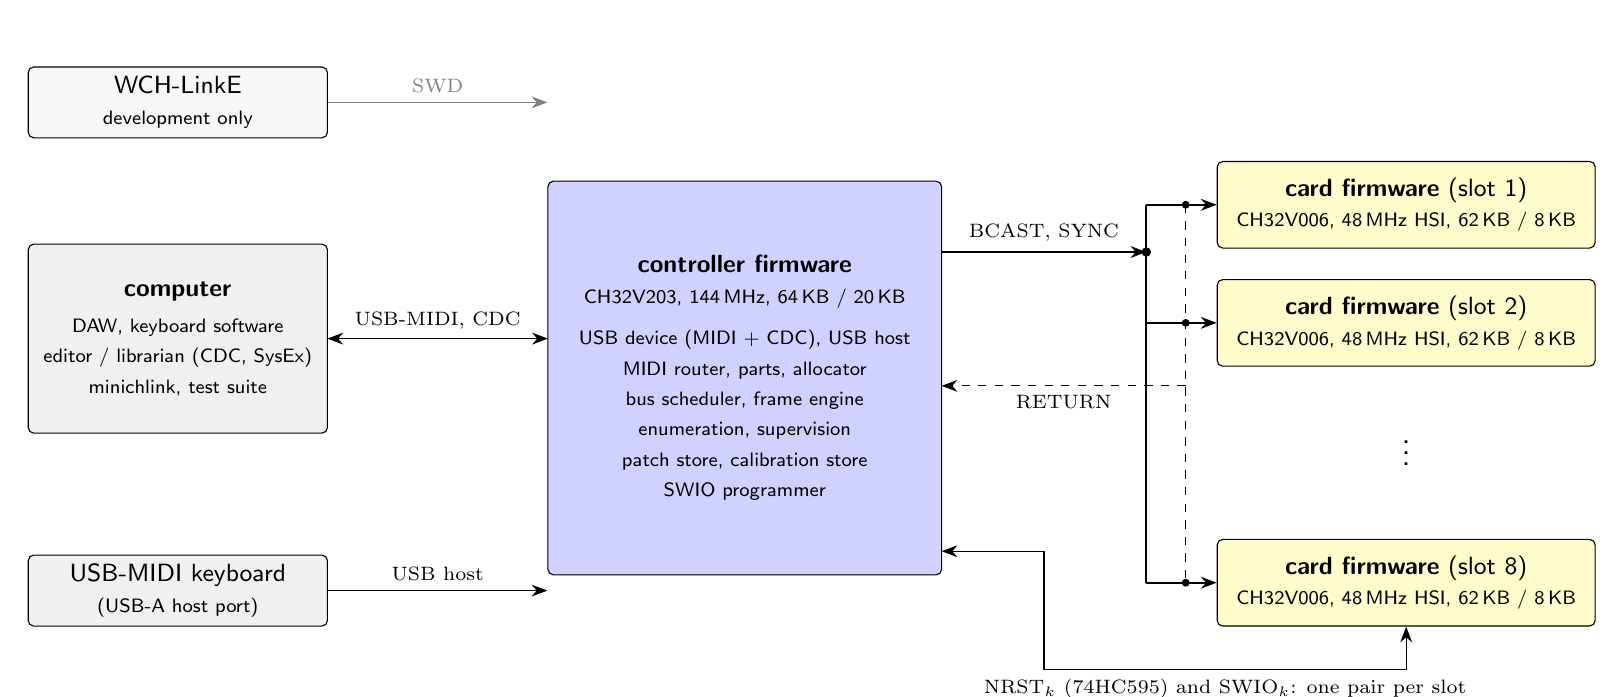
\begin{tikzpicture}[font=\small\sffamily, >={Stealth[length=2mm]},
  blk/.style={draw, rounded corners=2pt, fill=#1, minimum height=9mm, align=center}, blk/.default=white,
  lab/.style={font=\scriptsize}]
  \node[blk=gray!6, minimum width=38mm] (link) at (0,3.9) {WCH-LinkE\\\scriptsize development only};
  \node[blk=gray!12, minimum width=38mm, minimum height=24mm] (pc) at (0,0.9)
    {\textbf{computer}\\[2pt]\scriptsize DAW, keyboard software\\\scriptsize editor / librarian (CDC, SysEx)\\
     \scriptsize minichlink, test suite};
  \node[blk=gray!12, minimum width=38mm] (kbd) at (0,-2.3) {USB-MIDI keyboard\\\scriptsize (USB-A host port)};
  \node[blk=blue!18, minimum width=50mm, minimum height=50mm] (ct) at (7.2,0.4)
    {\textbf{controller firmware}\\\scriptsize CH32V203, 144\,MHz, 64\,KB / 20\,KB\\[4pt]
     \scriptsize USB device (MIDI + CDC), USB host\\\scriptsize MIDI router, parts, allocator\\
     \scriptsize bus scheduler, frame engine\\\scriptsize enumeration, supervision\\\scriptsize patch store,
     calibration store\\\scriptsize SWIO programmer};
  \foreach \n/\y in {1/2.6, 2/1.1, 8/-2.2}
    \node[blk=yellow!20, minimum width=48mm, minimum height=11mm] (c\n) at (15.6,\y)
      {\textbf{card firmware} (slot \n)\\\scriptsize CH32V006, 48\,MHz HSI, 62\,KB / 8\,KB};
  \node at (15.6,-0.45) {\large$\vdots$};
  \draw[<->] (1.9,0.9) -- node[above,lab]{USB-MIDI, CDC} (4.7,0.9);
  \draw[->] (kbd.east) -- node[above,lab]{USB host} (kbd.east -| ct.west);
  \draw[->, gray] (link.east) -- node[above,lab]{SWD} (link.east -| ct.west);
  \draw[->, thick] (9.7,2.0) -- node[above,lab]{BCAST, SYNC} (12.3,2.0);
  \draw[thick] (12.3,2.6) -- (12.3,-2.2);
  \foreach \n in {1,2,8} \draw[->, thick] (c\n.west -| 12.3,0) -- (c\n.west);
  \fill (12.3,2.0) circle (0.6mm);
  \draw[dashed] (12.8,2.6) -- (12.8,-2.2);
  \foreach \n in {1,2,8} \fill (c\n.west -| 12.8,0) circle (0.5mm);
  \draw[->, dashed] (12.8,0.3) -- node[below,lab]{RETURN} (9.7,0.3);
  \draw[<->] (9.7,-1.8) -- (11.0,-1.8) -- (11.0,-3.3) -- node[below,lab]{NRST$_k$ (74HC595) and SWIO$_k$: one pair
    per slot} (15.6,-3.3) -- (c8.south);
\end{tikzpicture}}
\caption{Software context. Two firmwares on nine microcontrollers. The computer plays and edits the instrument
over USB, and also runs the test suite and the programming tools during development. The controller is the only bus
master and the only owner of the instrument's state; each card runs one voice.}
\label{fig:sadctx}
\end{figure}

\begin{itemize}
  \item \textbf{Card firmware:} one image, identical on every card. A card knows nothing about its slot until it is
    enumerated, and it stores nothing except its calibration. It can be programmed by a WCH-LinkE (development, a card
    on its own) or by the controller over its SWIO line.
  \item \textbf{Controller firmware:} one image on the backplane. It holds the patches, the setups, the part
    configuration and the calibration copies, and is the time reference (crystal, SYNC). It is programmed over SWD
    or by the factory bootloader (BOOT0).
  \item \textbf{Host side:} no driver (class-compliant USB-MIDI, CDC ACM). The editor and librarian are not part
    of this project; CDC and SysEx are their interface.
\end{itemize}

% ---------------------------------------------------------------------------------------------------------------------
\subsection{Architectural drivers}

\begin{enumerate}
  \item \textbf{Alignment over latency} (P8, P10): every card must sound the same event at the same carrier period,
    independent of when its bytes arrive or what it is computing. A constant latency of a few milliseconds is
    acceptable.
  \item \textbf{One voice in \SI{48}{MHz} and \SI{8}{KB}} (C3): the DAC renderer needs one sample per
    \SI{5.33}{\micro s}, the control tick 1\,kHz, the bus parser up to 100 bytes per frame, all without a missed buffer
    half.
  \item \textbf{Robustness without acknowledgements:} lost packets, card resets, controller resets and missing SYNC
    edges must heal by themselves.
  \item \textbf{Testability on the bench:} one real card plus virtual voices must exercise the full protocol and load;
    timing must be observable through counters.
  \item \textbf{Updatable in the field:} cards from the controller, the controller from the computer.
\end{enumerate}

% ---------------------------------------------------------------------------------------------------------------------
\subsection{Principal decisions}

\begingroup\small\setlength{\tabcolsep}{4pt}
\begin{longtable}{@{}>{\raggedright}p{0.7cm} >{\raggedright}p{4.4cm} >{\raggedright}p{3.6cm}
  >{\raggedright\arraybackslash}p{6.9cm}@{}}
\caption{Architecture decisions.}\label{tab:sadadr}\\
\toprule
ID & Decision & Alternative & Reason, consequence \\
\midrule\endfirsthead
\toprule
ID & Decision & Alternative & Reason, consequence \\
\midrule\endhead
\bottomrule\endfoot
A1 & Time-triggered bus: events carry their execution frame ($a + L$); outputs follow $D$ frames later & events run on
  arrival & Alignment to one carrier period on every card, whatever the parse and render timing. Costs a constant
  5--7\,ms latency (P8 allows 10). \\
A2 & The controller owns all state; cards are stateless except for their calibration; periodic refreshes repair
  losses & an acknowledged protocol; patches stored on the cards & Broadcast stays simple, one card speaks at a time,
  a card can be swapped or reset at any time. Costs about 1.5 bytes per frame of refresh. \\
A3 & DAC render in the DMA half / complete interrupt at the low preemption level, with nesting; everything else at
  the high level & render in the main loop & A stall in the main loop (console) can never cost audio, and the tick
  enters within 27--28 cycles during a render. The render's budget must include the ticks that preempt it. \\
A4 & Bus parsing in the control tick, with early discard of foreign packets & parsing in the main loop below the
  render & Keeps $L = 2$. Affordable since the render rewrite (at least 99 periods of slack). The fallback, if card CPU
  becomes tight again, needs $L = 3$. \\
A5 & Bare metal on ch32fun: static buffers, no RTOS, no heap & FreeRTOS or similar & \SI{8}{KB} RAM, four execution
  contexts, deterministic timing; the stack is monitored instead (NF3). \\
A6 & One card code base for board~1 and the voice card (\texttt{BOARD}) & a separate card firmware & The engine,
  DSP and drivers stay tested on both; costs conditional code in \file{hw.c} and \file{board.h}. \\
A7 & The renderer is bit-exact against a reference revision; its hot loops are inline assembly, run from SRAM, and
  verified by an on-target hash & plain C; a half-rate render & Four to five times faster with an unchanged sound. The
  assembly is verified only by the hash, and the RAM code costs \SI{2.3}{KB}. \\
A8 & Controller USB: an own USBD driver and ch32fun's \file{fsusb.c} for USBFS behind one API, flow control by NAK &
  ch32fun \file{usbd.c}; TinyUSB & No message is lost, and DMA1 stays on (\file{usbd.c} switches it off). TinyUSB is
  reconsidered for the host port. \\
A9 & Cards are updated over SWIO from the controller (WCH one-wire debug protocol, bit-banged) & a bootloader on the
  card, over the bus & No card bootloader to maintain or to brick, and the same path as the WCH-LinkE (minichlink).
  Costs 8 controller GPIOs. \\
A10 & NRST through the 74HC595 without pull-downs; cards run freely while the controller is not running & cards held
  in reset & A controller reset or a debugger halt needs no special handling. The firmware must take the cards back
  (reset all, enumerate). \\
A11 & Each card trims its HSI to SYNC and scales its pitch by the measured frame period & a shared \SI{24}{MHz} clock &
  No clock distribution. The HSI's short-term wander (0.35\,cent rms) remains; CLK\_IN stays as an option. \\
A12 & The host software is a browser app (Web MIDI, Web Serial), static files without a build step & a Python
  desktop app; a DAW plugin (VST3, CLAP) & No installation on any system, works offline; the Python tools stay for
  automated tests. Needs a Chromium-based browser (Web Serial). \\
A13 & One parameter table (JSON) generates the app's parameter list, the controller firmware's tables and the docs'
  table & hand-kept copies & The app, the firmware and midi.md cannot drift apart. \\
\end{longtable}
\endgroup

% ---------------------------------------------------------------------------------------------------------------------
\subsection{Card firmware}\label{sec:sadcard}

\paragraph{Modules.} The card firmware has four layers. Each module calls only those below it, except for the
callbacks named in Table~\ref{tab:sadmod}.

\begin{table}[htbp]
\centering\small
\caption{Card firmware modules and their interfaces (\file{firmware/voice/}).}\label{tab:sadmod}
\begin{tabularx}{\textwidth}{@{}l l X@{}}
\toprule
Layer & Module & Responsibility; interface \\
\midrule
application & \file{touchsynth.c} & start-up, interrupt levels, the control tick dispatcher (\texttt{control\_tick}:
  bus, synth, CV commit, $V_n$ commit), SysTick fallback, main loop; stack monitor \\
 & \file{console.c} & SWIO console: diagnostics, manual control, render bench and check \\
protocol & \file{bus.c} & bus state machine (Figure~\ref{fig:sadstate}), HSI trim, frame counter, $\bar P$, in-place
  COBS / CRC parser, event queue, replies; \texttt{bus\_tick}, \texttt{bus\_present} \\
voice & \file{synth.c} & voice engine at \SI{1}{kHz} (envelopes, LFO, glide, CV laws), bus event handlers
  \texttt{synth\_bus\_*}, presets and tunes \\
 & \file{dsp.c} & DAC engines (oscillators, noise, modal), error feedback, $V_n$ queue and block split;
  \texttt{dsp\_pitch}, \texttt{dsp\_strike}, \texttt{dsp\_commit}, the render callback \texttt{dsp\_fill} \\
 & \file{tables.h} & generated: presets, CV laws, mode tables, exponential tables \\
drivers & \file{hw.c} & TIM1 CV PWM and its DMA burst, CV delay line; TIM2 DAC, ring and DMA ch1 with the render
  interrupt; SYNC EXTI; USART1 RX ring and TX by DMA; ADC capture; LEDs; chip ID \\
 & \file{board.h} & pin map and timer remaps per board and chip \\
platform & ch32fun & start-up code, register definitions, \texttt{funPinMode} \\
\bottomrule
\end{tabularx}
\end{table}

\paragraph{Execution contexts.} Table~\ref{tab:sadexec} lists every context with its trigger, level and measured
cost. The budget rule follows from A3: a buffer half's render time plus the ticks that preempt it must stay below
65\,536 cycles. The slack, in carrier periods, is what the counters report.

\begin{table}[htbp]
\centering\small
\caption{Card execution contexts (V006 at \SI{48}{MHz}; costs from the bench, Section~\ref{sec:cpu}).}\label{tab:sadexec}
\setlength{\tabcolsep}{4pt}
\begin{tabularx}{\textwidth}{@{}>{\raggedright}p{1.9cm} >{\raggedright}p{2.9cm} >{\raggedright}p{1.3cm} >{\raggedright}X >{\raggedright\arraybackslash}p{3.7cm}@{}}
\toprule
Context & Trigger, rate & Level & Work & Worst measured \\
\midrule
control tick & SYNC edge, EXTI4 (PD4), \SI{1}{kHz} & high & parse bytes received before the tick, run due
  events, replies; synth tick; CV commit; $V_n$ commit & 7\,k cycles idle, 9\,k at 71\,B/frame, 19\,k with a reply,
  27\,k at a modal PATCH\_SELECT \\
SysTick & only without SYNC (standalone, a missing edge) & high & the same tick & as above \\
DAC render & DMA1 ch1 half / complete, \SI{732}{Hz} & low & render the half that has just played: 256 periods in
  blocks of 32, split at $V_n$ boundaries & 8--12\,k (oscillators), 21\,k (modal); with preempting ticks 25\,k of
  65.5\,k \\
CV dither & TIM1 CC1 request at each update, \SI{46.875}{kHz} & DMA ch2 & 4-register burst from a 16-halfword table &
  no CPU \\
bus RX, TX & USART1 & DMA ch5, ch4 & receive ring of 256 bytes; replies & no CPU \\
main loop & -- & -- & SWIO console, stack low-water mark & -- \\
\bottomrule
\end{tabularx}
\end{table}

\paragraph{Data flow and the presentation delay.} Figure~\ref{fig:sadflow} follows one NOTE\_ON. It arrives during
frame $f-1$, the tick of frame $f$ parses it (its execution frame), and the voice engine computes the new state.
That state is delayed to frame $f + D$: the CVs through a delay line of $D + 1$ entries, the DAC state $V_f$ through a
queue stamped with $b_f = t_f + D\,\bar P$. The renderer splits its block at the carrier period of $b_f$, so the
change is exact to one period on every card.

\begin{figure}[htbp]
\centering
\resizebox{\textwidth}{!}{%
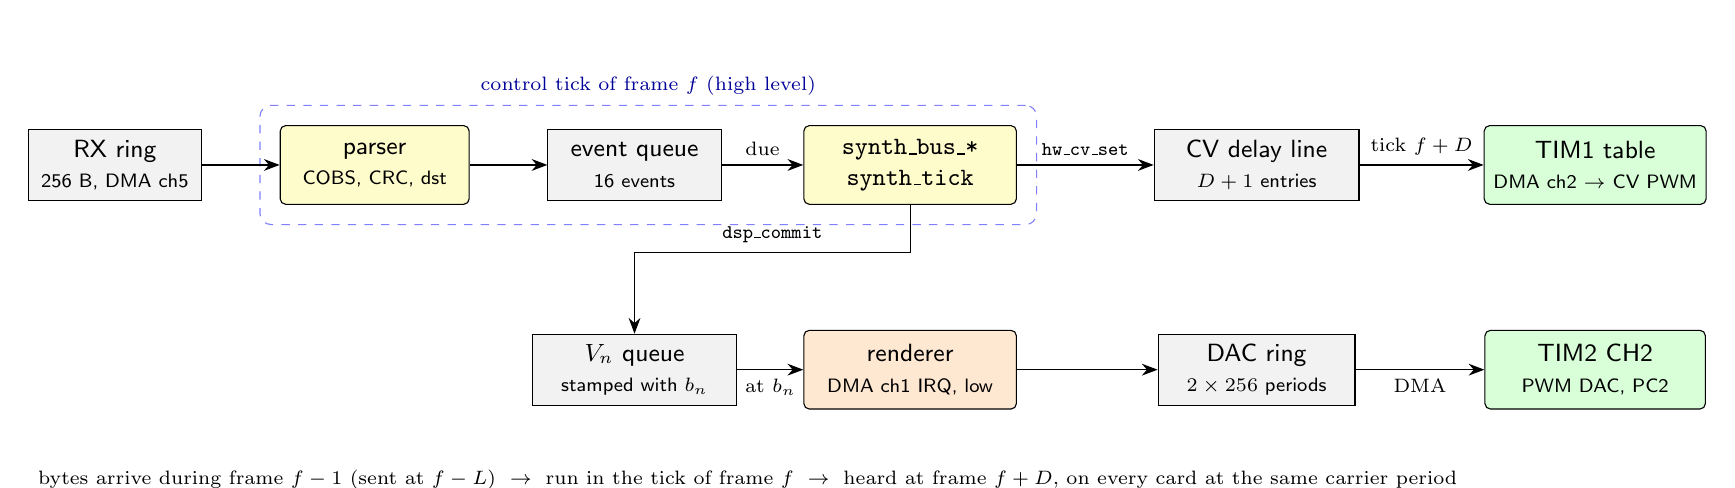
\begin{tikzpicture}[font=\small\sffamily, >={Stealth[length=2mm]},
  st/.style={draw, rounded corners=2pt, fill=#1, minimum height=10mm, minimum width=24mm, align=center},
  st/.default=white, buf/.style={draw, fill=gray!10, minimum height=9mm, minimum width=22mm, align=center},
  lab/.style={font=\scriptsize}]
  \node[buf] (ring) at (0,0) {RX ring\\\scriptsize 256 B, DMA ch5};
  \node[st=yellow!20] (parse) at (3.3,0) {parser\\\scriptsize COBS, CRC, dst};
  \node[buf] (evq) at (6.6,0) {event queue\\\scriptsize 16 events};
  \node[st=yellow!20, minimum width=27mm] (synth) at (10.1,0) {\texttt{synth\_bus\_*}\\\texttt{synth\_tick}};
  \node[buf, minimum width=26mm] (cvl) at (14.5,0) {CV delay line\\\scriptsize $D+1$ entries};
  \node[st=green!15, minimum width=28mm] (tim1) at (18.8,0) {TIM1 table\\\scriptsize DMA ch2 $\to$ CV PWM};
  \node[buf, minimum width=26mm] (vq) at (6.6,-2.6) {$V_n$ queue\\\scriptsize stamped with $b_n$};
  \node[st=orange!18, minimum width=27mm] (rend) at (10.1,-2.6) {renderer\\\scriptsize DMA ch1 IRQ, low};
  \node[buf, minimum width=25mm] (dring) at (14.5,-2.6) {DAC ring\\\scriptsize $2\times256$ periods};
  \node[st=green!15, minimum width=28mm] (tim2) at (18.8,-2.6) {TIM2 CH2\\\scriptsize PWM DAC, PC2};
  \draw[->] (ring) -- (parse); \draw[->] (parse) -- (evq);
  \draw[->] (evq) -- node[above,lab]{due} (synth);
  \draw[->] (synth) -- node[above,lab]{\texttt{hw\_cv\_set}} (cvl);
  \draw[->] (cvl) -- node[above,lab]{tick $f+D$} (tim1);
  \draw[->] (synth.south) -- ++(0,-0.6) -| node[pos=0.25,above,lab]{\texttt{dsp\_commit}} (vq.north);
  \draw[->] (vq) -- node[below,lab]{at $b_n$} (rend);
  \draw[->] (rend) -- (dring);
  \draw[->] (dring) -- node[below,lab]{DMA} (tim2);
  \begin{scope}[on background layer]
    \node[draw=blue!50, dashed, rounded corners, fit=(parse)(evq)(synth), inner sep=2.5mm,
      label={[lab, blue!60!black]above:control tick of frame $f$ (high level)}] {};
  \end{scope}
  \node[lab, anchor=west, align=left] at (-1.1,-4.0) {bytes arrive during frame $f-1$ (sent at $f-L$) $\;\to\;$ run in
    the tick of frame $f$ $\;\to\;$ heard at frame $f+D$, on every card at the same carrier period};
\end{tikzpicture}}
\caption{Card data flow from a received event to the outputs. Buffers are grey; the dashed box runs in the control
tick, the renderer in the low-level DMA interrupt.}
\label{fig:sadflow}
\end{figure}

\paragraph{Bus state machine.} Figure~\ref{fig:sadstate} shows the card's states, as implemented in \file{bus.c}.
Each state's outputs: in STANDALONE the voice plays from the console or its tunes; in TRIM and LISTEN the receiver is
being prepared; in SYNCED timed events run; in LOST the VCA is muted until SYNC returns.

\begin{figure}[htbp]
\centering
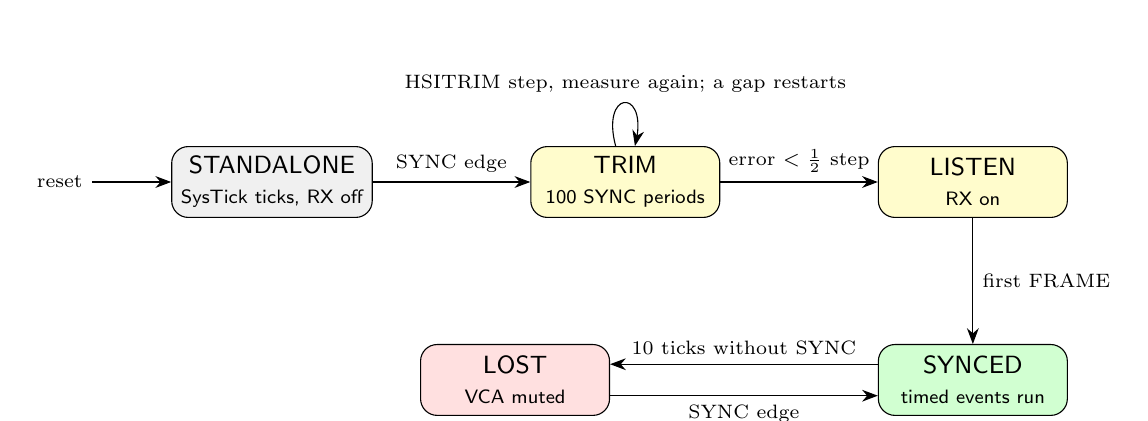
\begin{tikzpicture}[font=\small\sffamily, >={Stealth[length=2mm]}, node distance=8mm and 20mm,
  s/.style={draw, rounded corners=6pt, fill=#1, minimum height=9mm, minimum width=24mm, align=center},
  s/.default=white, lab/.style={font=\scriptsize, align=center}]
  \node[s=gray!12] (sa) {STANDALONE\\\scriptsize SysTick ticks, RX off};
  \node[s=yellow!20, right=of sa] (tr) {TRIM\\\scriptsize 100 SYNC periods};
  \node[s=yellow!20, right=of tr] (li) {LISTEN\\\scriptsize RX on};
  \node[s=green!18, below=16mm of li] (sy) {SYNCED\\\scriptsize timed events run};
  \node[s=red!12, left=34mm of sy] (lo) {LOST\\\scriptsize VCA muted};
  \draw[->] ([xshift=-10mm]sa.west) node[left,lab]{reset} -- (sa);
  \draw[->] (sa) -- node[above,lab]{SYNC edge} (tr);
  \draw[->] (tr) to[loop above] node[above,lab]{HSITRIM step, measure again; a gap restarts} (tr);
  \draw[->] (tr) -- node[above,lab]{error $<\frac12$ step} (li);
  \draw[->] (li) -- node[right,lab]{first FRAME} (sy);
  \draw[->] ([yshift=2mm]sy.west) -- node[above,lab]{10 ticks without SYNC} ([yshift=2mm]lo.east);
  \draw[->] ([yshift=-2mm]lo.east) -- node[below,lab]{SYNC edge} ([yshift=-2mm]sy.west);
\end{tikzpicture}
\caption{Card bus states (\file{bus.c}). A missing SYNC edge is bridged by a SysTick tick and counted (it
does not leave SYNCED); an NRST or SWIO reset restarts at STANDALONE.}
\label{fig:sadstate}
\end{figure}

\paragraph{Memory.} Table~\ref{tab:sadmem} gives the card build's memory (link map of the current build). The DAC
ring, the renderer's work area and the console's capture buffer share one buffer (\texttt{hw\_scratch}): captures are
refused while the DAC runs.

\begin{table}[htbp]
\centering\small
\caption{Card build memory (CH32V006, \texttt{make BOARD=card}).}\label{tab:sadmem}
\begin{tabularx}{\textwidth}{@{}l r X@{}}
\toprule
Item & Bytes & Content \\
\midrule
flash: code and constants & 53\,228 & of 63\,488; plus the \texttt{.data} image: \SI{55.6}{KB} in all \\
RAM \texttt{.data} & 2\,416 & initialised data and about \SI{2.3}{KB} of render code run from SRAM \\
RAM \texttt{.bss} & 4\,608 & \texttt{hw\_scratch} 2560 (DAC ring 512, render work area 256, console capture);
  modal voices 760; RX ring 256; event queue 128; $V_n$ queue 128; CV delay line 78; packet and reply buffers 128;
  oscillator state 72; bus, patch and CV burst state 118; the rest small \\
stack region & 1\,168 & at least 656 bytes never used under bus load and stress, about 340 with the console \\
\bottomrule
\end{tabularx}
\end{table}

% ---------------------------------------------------------------------------------------------------------------------
\subsection{Controller firmware}\label{sad:ctrl}

\paragraph{Modules.} Table~\ref{tab:sadctmod} lists the controller's target modules (from \file{docs/controller.md})
and what the bench stand-in already provides.

\begingroup\small\setlength{\tabcolsep}{4pt}
\begin{longtable}{@{}>{\raggedright}p{3.0cm} >{\raggedright}p{7.6cm} >{\raggedright\arraybackslash}p{4.9cm}@{}}
\caption{Controller firmware modules: target and bench status.}\label{tab:sadctmod}\\
\toprule
Module & Responsibility & In \file{bench\_ctrl} \\
\midrule\endfirsthead
\toprule
Module & Responsibility & In \file{bench\_ctrl} \\
\midrule\endhead
\bottomrule\endfoot
frame engine & TIM1 CH1 SYNC; at each edge FRAME, enumeration, queued packets up to 95 bytes, refreshes; one TX DMA
  transfer & built \\
bus scheduler & stamps events with $a + L$; two queues (notes, then controllers); coalescing; late accounting &
  built (no coalescing) \\
reply handler & RX DMA ring on RETURN; COBS / CRC; HELLO, STATUS, COUNTERS, CAL\_DATA; time-outs & built \\
slot manager & 595 reset and release, enumeration, chip ID $\to$ slot, supervision and recovery (NRST, SWIO) & one
  slot, without NRST \\
USB device & composite USB-MIDI + CDC: USBD driver (backplane), USBFS driver (development board) & built (USBD
  enumerated by the own host) \\
USB host & class-compliant MIDI on USBFS, power switch and fault & built (\texttt{USBH=1}, \file{usbhost.c};
  self-loop tested, no hubs) \\
MIDI input & per port: running status, real time, SysEx assembly; ports: USB-MIDI, USB host, USART1 (DIN option) &
  USB-MIDI and the bench command \\
part router & channel and key range $\to$ part; CC, NRPN and sustain handling; program change; MIDI clock & one
  poly part, or one part per channel \\
allocator & voice choice within a slot mask; PATCH\_SELECT and PATCH\_DATA before a NOTE\_ON; unison and kit modes &
  basic allocator \\
patch store & 64 programs and setups in flash pages with wear levelling; working copies in SRAM & -- \\
calibration store & CAL\_DATA by chip ID & -- \\
CDC commands & text commands of midi.md 6; SysEx dumps & binary bench command set, identity reply \\
SWIO programmer & WCH one-wire protocol (bit-banged, \SI{125}{ns} resolution) on 8 lines; image from CDC, program and
  verify & Ardulink bridge for minichlink (one line) \\
supervision & watchdog; VBUS\_DET and the D+ pull-up; activity LED & -- \\
options & UAC1 audio from the ADC taps; CLK\_OUT on TIM3 CH4 & -- \\
\end{longtable}
\endgroup

\paragraph{Execution contexts.} The frame interrupt (TIM1 update, at the SYNC rising edge) has the highest priority
and builds each frame's transmission from queues filled by the main loop. Its budget is \SI{40}{\micro s} from the
edge to the start of the DMA; measured 0--3\,\textmu s with and without USB traffic. The USB interrupt has a lower
priority, and interrupt nesting is off, so USB can only delay the frame interrupt by its own length (at most
\SI{3}{\micro s} measured). The main loop serves the command ports, turns USB-MIDI packets into events, runs the
allocator and, in the target design, the storage and programming tasks. A flash erase or a SWIO programming run must
not hold up the queues: both run in the main loop between frames, and the frame interrupt keeps sending refreshes.

\begin{figure}[htbp]
\centering
\resizebox{\textwidth}{!}{%
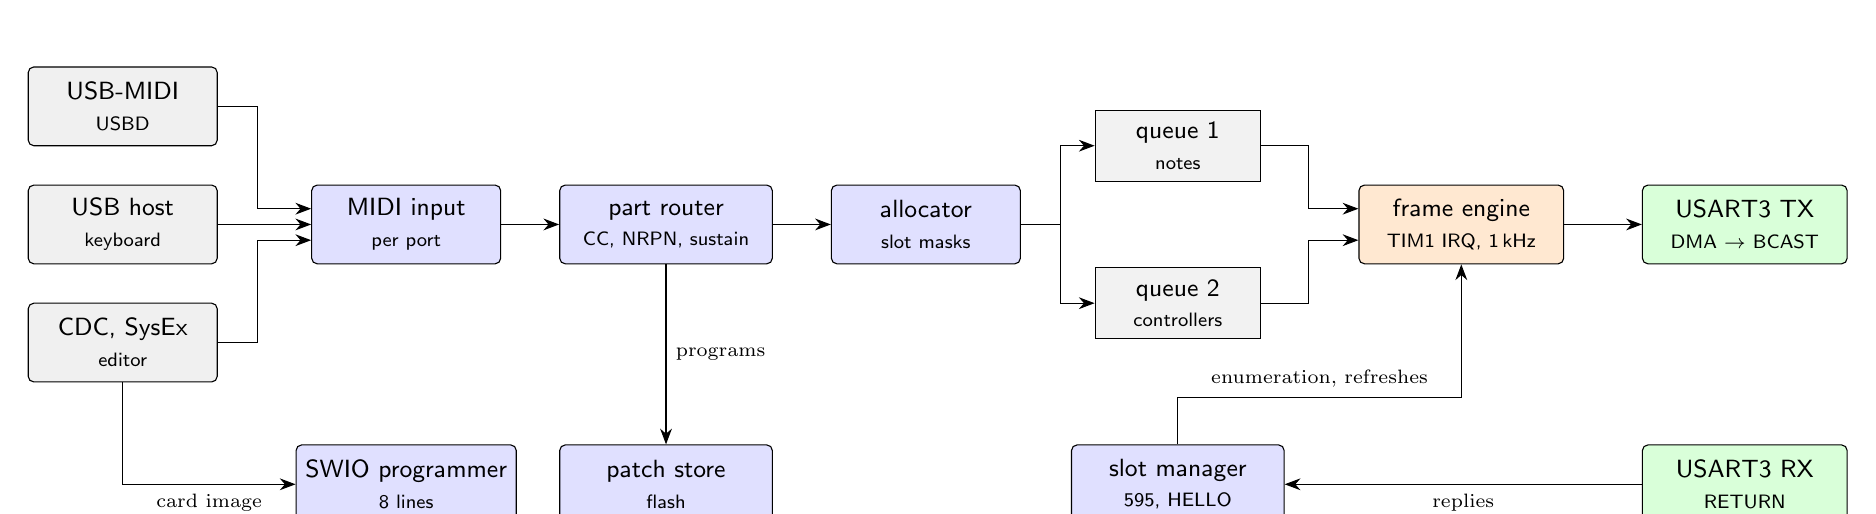
\begin{tikzpicture}[font=\small\sffamily, >={Stealth[length=2mm]},
  st/.style={draw, rounded corners=2pt, fill=#1, minimum height=10mm, minimum width=24mm, align=center},
  st/.default=white, buf/.style={draw, fill=gray!10, minimum height=9mm, minimum width=21mm, align=center},
  lab/.style={font=\scriptsize}]
  \node[st=gray!12] (usbd) at (0,1.5) {USB-MIDI\\\scriptsize USBD};
  \node[st=gray!12] (host) at (0,0) {USB host\\\scriptsize keyboard};
  \node[st=gray!12] (cdc) at (0,-1.5) {CDC, SysEx\\\scriptsize editor};
  \node[st=blue!12] (midi) at (3.6,0) {MIDI input\\\scriptsize per port};
  \node[st=blue!12, minimum width=27mm] (parts) at (6.9,0) {part router\\\scriptsize CC, NRPN, sustain};
  \node[st=blue!12] (alloc) at (10.2,0) {allocator\\\scriptsize slot masks};
  \node[buf] (q1) at (13.4,1.0) {queue 1\\\scriptsize notes};
  \node[buf] (q2) at (13.4,-1.0) {queue 2\\\scriptsize controllers};
  \node[st=orange!18, minimum width=26mm] (fe) at (17.0,0) {frame engine\\\scriptsize TIM1 IRQ, 1\,kHz};
  \node[st=green!15, minimum width=26mm] (tx) at (20.6,0) {USART3 TX\\\scriptsize DMA $\to$ BCAST};
  \node[st=blue!12, minimum width=27mm] (swio) at (3.6,-3.3) {SWIO programmer\\\scriptsize 8 lines};
  \node[st=blue!12, minimum width=27mm] (store) at (6.9,-3.3) {patch store\\\scriptsize flash};
  \node[st=blue!12, minimum width=27mm] (slot) at (13.4,-3.3) {slot manager\\\scriptsize 595, HELLO};
  \node[st=green!15, minimum width=26mm] (rx) at (20.6,-3.3) {USART3 RX\\\scriptsize RETURN};
  \draw[->] (usbd.east) -- ++(0.5,0) |- ([yshift=2mm]midi.west);
  \draw[->] (host.east) -- (midi.west);
  \draw[->] (cdc.east) -- ++(0.5,0) |- ([yshift=-2mm]midi.west);
  \draw[->] (midi) -- (parts); \draw[->] (parts) -- (alloc);
  \draw[->] (alloc.east) -- ++(0.5,0) |- (q1.west);
  \draw[->] (alloc.east) -- ++(0.5,0) |- (q2.west);
  \draw[->] (q1.east) -- ++(0.6,0) |- ([yshift=2mm]fe.west);
  \draw[->] (q2.east) -- ++(0.6,0) |- ([yshift=-2mm]fe.west);
  \draw[->] (fe) -- (tx);
  \draw[->] (parts.south) -- node[right,lab]{programs} (store.north);
  \draw[->] (rx.west) -- node[below,lab]{replies} (slot.east);
  \draw[->] (slot.north) -- ++(0,0.6) -| node[pos=0.25,above,lab]{enumeration, refreshes} (fe.south);
  \draw[->] (cdc.south) |- node[pos=0.75,below,lab]{card image} (swio.west);
\end{tikzpicture}}
\caption{Controller data flow (target). Blue modules run in the main loop, the frame engine in the frame interrupt.}
\label{fig:sadctflow}
\end{figure}

\paragraph{Start-up sequence.} Clocks and USB; shift 0x00 into the 595 and enable its outputs (all cards in reset);
start SYNC and FRAME; enumerate slot by slot (bus.md 6); send CONFIG and the active patches; then start USB-MIDI
processing. A controller reset at any point restarts this sequence; the cards run muted in the meantime (A10).

\paragraph{Storage (proposed).} Flash pages for 64 programs of 144 bytes (\SI{9.2}{KB}), 8 setups and the
calibration copies (8 cards $\times$ about 64 bytes), written by appending to a log with a sequence number and a CRC
and compacted when full. The working copies in SRAM are what the parts use. A corrupt or empty store falls back to
built-in defaults.

% ---------------------------------------------------------------------------------------------------------------------
\subsection{Host software}\label{sec:sadhs}

The browser app (requirements in Section~\ref{sec:srshs}) is a set of static files in the repository (\file{app/};
first version 2026-10-20): plain HTML and JavaScript without a build step and without modules (Chromium blocks
module scripts from \texttt{file://}), so it opens from disk or from any static web server and works offline (A12).
An emulated instrument (programs, parts, six voice cards, voice allocation, Web Audio sound) stands in for the
hardware; the tests run in Node (protocol and emulator) and in headless Edge (an offline render of the sound). Its
layers:

\begin{table}[htbp]
\centering\small
\caption{Host software modules (\file{app/js/}).}\label{tab:sadhs}
\begin{tabularx}{\textwidth}{@{}l X@{}}
\toprule
Module & Responsibility \\
\midrule
MIDI link & Web MIDI: find the instrument's ports, send NRPN and SysEx, receive replies and incoming notes; SysEx
  framing and checksums \\
serial link & Web Serial on the CDC port: the maintenance commands, firmware image transfer, the console bridge \\
instrument model & the state mirrored from the instrument: active patch, programs, parts, cards and their status;
  every view reads and changes it, the links keep it in sync \\
parameter table & generated from the shared JSON (A13): IDs, names, ranges, units, CC numbers, grouping for the
  editor \\
views & patch editor, librarian, setup (parts), instrument view, maintenance, keyboard and MIDI monitor \\
files & import and export of \texttt{.syx} patches and banks, firmware images chosen by the user \\
\bottomrule
\end{tabularx}
\end{table}

\paragraph{Protocol split.} Everything musical goes over MIDI, so a DAW or any MIDI host reaches the same functions
(CT13): live parameter changes as NRPN (midi.md 3), patches, banks, setups, parts, card status and calibration as
SysEx messages with the non-commercial ID 0x7D, each with a request and a reply. Maintenance goes over the CDC port:
firmware images for the cards (programmed by the controller over SWIO) and for the controller, the console bridge
to one card, bulk diagnostics. The SysEx message set is drafted in \file{docs/sysex.md} (implemented by the
emulator); the maintenance commands are to be specified with the controller firmware.

\paragraph{Development path.} The app can be written and tested against the bench controller before the backplane
exists: it already is a USB-MIDI and CDC device, and the browser on the lab PC reaches both. The SysEx and NRPN
handling then moves with the controller firmware from the bench to the backplane unchanged.

% ---------------------------------------------------------------------------------------------------------------------
\subsection{Interfaces}

\begin{table}[htbp]
\centering\small
\caption{Software interfaces.}\label{tab:sadif}
\begin{tabularx}{\textwidth}{@{}l l X@{}}
\toprule
Interface & Between & Specification and state \\
\midrule
voice bus & controller, cards & \file{docs/bus.md} 2--6 (0.2, implemented; card firmware version 3) \\
patch parameter IDs & controller, cards, editor & \file{docs/midi.md} 4 (proposal; the cards implement a subset) \\
USB-MIDI & computer, controller & class compliant, one cable each way; \file{docs/controller.md} 5. USB ID 1209:0001
  is a test ID for development only \\
CDC & computer, controller & bench: binary commands (\file{bench\_ctrl.c} header); target: text commands
  (\file{docs/midi.md} 6, to define) \\
SysEx & computer, controller & ID 0x7D: identity reply implemented; patches, banks, setups, parts, card status
  and calibration to define (Section~\ref{sec:sadhs}) \\
NRPN & computer, controller & live parameter changes, IDs of midi.md 4 (from the shared parameter table, A13) \\
Web MIDI, Web Serial & browser app, computer & the app's access to the instrument's MIDI and CDC ports \\
SWIO console & computer, card & \file{console.c} commands (\file{firmware/voice/README.md}) \\
Ardulink & computer, controller & minichlink's Ardulink programmer protocol, for card programming through the
  controller \\
generated tables & tools, card firmware & \file{tables.h} from the result files (\file{gen\_tables.py}) \\
\bottomrule
\end{tabularx}
\end{table}

% ---------------------------------------------------------------------------------------------------------------------
\subsection{Build variants}

\begin{table}[htbp]
\centering\small
\caption{Build variants.}\label{tab:sadbuild}
\begin{tabularx}{\textwidth}{@{}l l X@{}}
\toprule
Firmware & Option & Effect \\
\midrule
card & \texttt{BOARD=card} & the voice card's pin map and the bus receiver (default: board~1 with its DCO and MIDI
  input) \\
 & \texttt{BUS\_TX\_PP=1} & bench only: the return line driven push-pull during a reply (no \SI{1}{k\ohm} pull-up on
  the bench) \\
 & \texttt{BUS\_BAUD=2000000} & \SI{2}{Mbaud} bus (both firmwares must match) \\
 & \texttt{DAC\_DUAL=1} & dual-PWM DAC (high and low byte, PC1) \\
 & chip & CH32V006 (card, board~1 with a V006); V003 and V002 builds compile \\
controller (bench) & \texttt{USB=usbd} & USB on USBD, PA11 / PA12 (the backplane's port; default USBFS on the
  development board) \\
 & \texttt{BUS\_BAUD=2000000} & as above \\
\bottomrule
\end{tabularx}
\end{table}

% ---------------------------------------------------------------------------------------------------------------------
\subsection{Verification architecture}

The software is verified at five levels (Table~\ref{tab:sadver}). Each requirement of Section~\ref{sec:srs} names
the level that covers it; Table~\ref{tab:srssum} summarises their status.

\begin{table}[htbp]
\centering\small
\caption{Verification levels.}\label{tab:sadver}
\begin{tabularx}{\textwidth}{@{}l l X@{}}
\toprule
Level & Tool & Covers \\
\midrule
model & \file{sim/behav/} (\file{dsp.py}, \file{behav.py}) & algorithms and sound, against the analog model (S9) \\
host regression & \file{firmware/voice/test/render\_test.py} & the renderer bit-exact against a reference revision,
  197 scenarios \\
on target & console \texttt{check}, \texttt{bench} & assembly and compiler (hash), cycle counts per patch \\
bench integration & \file{tools/bustest.py}, \file{tools/usbtest.py} & protocol, timing, latency, errors, load with 7
  virtual voices, USB-MIDI and CDC; V203 development board and one V006 \\
system & stages V2--V4 (Table~\ref{tab:vstages}) & real cards and backplane: NRST, alignment between cards,
  calibration, 8 cards \\
\bottomrule
\end{tabularx}
\end{table}

\begin{table}[htbp]
\centering\small
\caption{Status of the software requirements (Section~\ref{sec:srs}), 20 October 2026.}\label{tab:srssum}
\begin{tabular}{@{}l r r r r r@{}}
\toprule
Group & Requirements & met & partial & open & design \\
\midrule
card firmware (CF) & 23 & 16 & 4 & 3 & 0 \\
voice bus (BUS) & 8 & 5 & 1 & 0 & 2 \\
controller firmware (CT) & 22 & 2 & 11 & 8 & 1 \\
tools, non-functional (TL, NF) & 8 & 8 & 0 & 0 & 0 \\
host software (HS) & 11 & 1 & 9 & 1 & 0 \\
\midrule
all & 72 & 32 & 25 & 12 & 3 \\
\bottomrule
\end{tabular}
\end{table}

% ---------------------------------------------------------------------------------------------------------------------
\subsection{Open architecture questions}\label{sec:sadopen}

\begin{enumerate}
  \item \textbf{USB stack for the host port.} Extend the own drivers (A8) to a minimal MIDI host, or port TinyUSB
    for both ports? The host port is fitted now, and a minimal MIDI host on the own drivers works in a self-loop on
    the development board (Section~\ref{sec:fw}); TinyUSB would add hubs and more device classes.
  \item \textbf{Parsing location (A4).} Stay with parsing in the tick ($L = 2$), or move it to the main loop now
    ($L = 3$, one more millisecond of latency) to decouple the bus load from the render for good?
  \item \textbf{CDC protocol.} Musical functions go over MIDI and maintenance over CDC (decided, 2026-10-20). Open:
    the maintenance commands as text or binary, and whether the bench's binary command set stays for the tests.
  \item \textbf{USB identity.} 1209:0001 is the pid.codes test ID. A product ID (pid.codes or another VID) is
    needed before the instrument leaves the bench.
  \item \textbf{Controller self-update.} The factory bootloader through BOOT0 (untested on the USB-C port), or an
    update mode in the firmware over CDC with a small resident loader?
  \item \textbf{Card firmware compatibility.} With cards updated one by one, should the controller refuse to start
    cards with a different firmware version (HELLO) or update them automatically?
\end{enumerate}


% =====================================================================================================================
\section{Firmware}\label{sec:fw}

\subsection{Voice card firmware}
The card firmware (\file{firmware/voice/}) grew out of the TouchSynth rev 0.1 firmware on ch32fun; the touch UI is removed, the board~1 build keeps the analog-DCO
code and its MIDI input. One code base builds for board~1 and, with \texttt{make BOARD=card}, for the card's pin map
with the bus receiver.
\begin{table}[htbp]
\centering\small
\caption{Card firmware modules.}\label{tab:fwmod}
\begin{tabularx}{\textwidth}{@{}l X@{}}
\toprule
File & Content \\
\midrule
\file{board.h} & pin maps (board~1, card), timer remap codes \\
\file{touchsynth.c} & main loop, control tick (SYNC edge on the card, SysTick on board~1), interrupt levels \\
\file{hw.c} & TIM1 CV PWM with 2-bit dither (DMA burst on the card), TIM2 DAC with its DMA ring and start sequence, SYNC EXTI, USART1 bus
  receiver (DMA ring) and transmitter, loopback ADC capture \\
\file{dsp.c} & oscillators (polyBLEP saw / pulse, noise), modal drum engine in fixed point, second-order error feedback,
  the $V_n$ queue and the block split of the presentation delay, pitch lock to SYNC; the hot loops run from SRAM,
  partly in assembly \\
\file{dsp\_check.h}, \file{test/} & render check (console \texttt{check}) and the host test of the renderer against a
  reference revision \\
\file{synth.c} & voice engine at \SI{1}{kHz}: glide, LFO, envelopes, CV laws, pitch envelope, bus event handlers \\
\file{bus.c} & voice bus: frame counter, HSI trim, COBS / CRC parser, event queue, replies \\
\file{console.c} & test console over SWIO (\texttt{minichlink -T}) \\
\file{tables.h} & generated by \file{gen\_tables.py} from the result files and the presets \\
\bottomrule
\end{tabularx}
\end{table}

\paragraph{Interrupt levels.} The V006 has two preemption levels with nesting (INTSYSCR.INESTEN). The DAC render runs
at the low level, everything else at the high level (Table~\ref{tab:irq}), so the control tick, the CV PWM and the
UART preempt a render, and a render preempts the main loop. Measured on board~1: the tick enters within 27--28
cycles while a render runs; without nesting it waited up to 45\,k cycles.

\begin{table}[htbp]
\centering\small
\caption{Card firmware timing.}\label{tab:irq}
\begin{tabularx}{\textwidth}{@{}l l l X@{}}
\toprule
Context & Rate & Level & Work \\
\midrule
TIM1 update & \SI{46.875}{kHz} & DMA & dithered CV PWM: 10 bit + 2-bit dither on four channels, a DMA burst on the
  card (board~1: an interrupt at the high level) \\
Control tick & \SI{1}{kHz} & high & the SYNC edge (EXTI on PD4); SysTick only while SYNC is missing: bus parsing and due
  events, synth tick, CV commit, $V_n$ commit \\
DMA1 ch1 half / complete & \SI{732}{Hz} & low & render the 256-period buffer half that has just played (oscillators
  or modal engine), at most 32 periods per block \\
Main loop & -- & -- & SWIO console \\
\bottomrule
\end{tabularx}
\end{table}

\paragraph{DAC rendering.} The DAC ring holds two halves of 256 carrier periods (512 bytes for single PWM, 1536 for
dual). At each half or complete transfer the renderer fills the half that has just played. It works in blocks of 32
periods, splits a block where a queued $V_n$ takes effect, and runs the error feedback over the block. The modal patch
uses 252-period halves (21 samples of 12 periods). If a $V_n$ arrives after its time it is applied at the start of the
half and counted as a late tick.

\paragraph{Render loops (2026-10-20).} Measured on the V006 with code in SRAM, an ALU operation or \texttt{mul} takes
1 cycle, \texttt{mulh(u)} 1--1.25, a load 2, a store 3 and a taken branch 3, so the renderer is built to avoid stores
and branches. Between the polyBLEP regions around a wrap or an edge a saw is \texttt{(ph >> 16)}$\,\cdot\,$level and a
pulse a constant; the oscillators of a patch are therefore rendered together in runs between those regions, with one
store per sample, and the samples within one step of a region take the full polyBLEP. The error feedback keeps the
error plus half a code, so one compare replaces four clamps. The run loops and the modal engine's free-ringing loop
are in inline assembly (with RV32E's 16 registers the compiler reloaded values from the stack), the modal resonators
are stored interleaved with alternating outputs, and about \SI{2.3}{KB} of render code runs from SRAM. The output is
bit-exact with the previous renderer: \file{firmware/voice/test/render\_test.py} compiles both on the host and
compares the duty codes of 197 scenarios (all DSP patches, test patches, notes 24--127, vibrato, glides, resets, modal
strikes), and the card's console command \texttt{check} prints a hash of a fixed render that matches the host's,
which covers the assembly and the target compiler. The fused sum relies on a patch's oscillator levels adding up to
at most 1, which \file{gen\_tables.py} checks.

\paragraph{Control tick.} On the card, each SYNC edge runs, in order:
\begin{enumerate}
  \item the bus tick: frame counter, SYNC period filter, HSI trim at start-up, SYNC loss detection, parsing of the
    bytes that arrived before the tick, and the events due in this frame;
  \item \texttt{synth\_tick}: envelopes, LFO, glide and the CV laws;
  \item the CV commit into the $D$-tick delay line;
  \item the $V_n$ commit with its presentation time.
\end{enumerate}
The parser drops packets for other cards at their dst byte, before the CRC, and skips to the next 0x00; the COBS
decoder runs over the RX ring in place. A REQUEST is answered in the tick that parses it, by TX DMA.

\paragraph{Memory.} On board~1 the phase-1 voice firmware used \SI{50.1}{KB} of \SI{62}{KB} flash and \SI{6.94}{KB}
of static RAM, including a \SI{4}{KB} console capture buffer that also holds the DAC ring. The card build gives
\SI{512}{bytes} of that buffer to the bus (RX ring, event queue). It takes about \SI{54}{KB} of flash and
\SI{7.3}{KB} of the \SI{8}{KB} RAM; the free stack stayed at 150--200 bytes under bus load (smallest seen: 156).
Since the render rewrite the card build takes about \SI{55}{KB} of flash and \SI{7.0}{KB} of static RAM: the shared
capture buffer shrank from 3584 to 2560 bytes (console captures of 1280 samples) to make room for the render code in
SRAM, the oscillator block buffer and the mallet table share it after the DAC ring, and 650--680 bytes of stack stay
free under bus load and the stress test (about 340 with the console attached). Board~1's buffer went from 4096 to
3584 bytes (\SI{7.5}{KB} static RAM); that build is not yet retested on hardware.

\subsection{Controller firmware}
The controller firmware for the backplane is planned in \file{docs/controller.md}; most of it is not written yet:
\begin{itemize}
  \item USB device (MIDI + CDC first, UAC1 audio later; running on the bench, below) and USB host (class-compliant
    MIDI);
  \item MIDI router and parts (8 parts, channels, key ranges, CCs, NRPN, program change, MIDI clock;
    \file{docs/midi.md});
  \item voice allocator (free voice, else the oldest released, else the oldest held, within a part's slot mask);
  \item bus scheduler (frame clock, timed events with lead $L$, refreshes, requests);
  \item enumeration and calibration storage by chip ID, patch library in flash, the SWIO programmer.
\end{itemize}
Today \file{firmware/bench\_ctrl} stands in for it on a CH32V203 development board. It runs from the \SI{8}{MHz}
crystal at \SI{144}{MHz} and provides:
\begin{itemize}
  \item the frame engine: in the TIM1 update interrupt (the SYNC rising edge) FRAME first, then enumeration and refresh
    packets, then queued packets up to a budget of 95 bytes per frame, one DMA transfer per frame;
  \item a command interface on USART1 (raw bytes, MIDI messages, packet bodies with corrupt-CRC options, requests,
    status, CONFIG, a scope marker on the SYNC pulse, SYNC gap tests, and the 8-voice load generator);
  \item an Ardulink-compatible SWIO bridge: \texttt{minichlink -C ardulink} flashes and debugs a CH32V006 through the
    V203, the path the backplane will use to update the cards. The one-wire protocol is bit-banged at \SI{125}{ns}
    resolution from the \SI{144}{MHz} SysTick.
\end{itemize}

\paragraph{USB (bench, 2026-10-19).} The development board's USB-C is wired to the V203's USBFS peripheral (PB6/PB7),
not to USBD (PA11/PA12), which the backplane uses for its device port. \file{bench\_ctrl} is now a full-speed composite
device on USBFS: class-compliant USB-MIDI (one cable each way; Linux binds \texttt{snd-usb-audio}) plus a CDC serial
port that carries the whole command set, the SWIO bridge included. Incoming USB-MIDI packets enter the same MIDI to
bus path as the serial command, with flow control (the host is held off when the buffers are full). Measured:
enumeration at the first attempt; the 17 bus checks pass over USART1 and over the CDC port; USB packet to execution
frame 1.0--2.0\,ms, so a note sounds 5.0--6.0\,ms after its USB packet at $D = 4$, $L = 2$; SYNC timing unchanged by
USB traffic (0.6--0.9\,ns, the scope's resolution); re-plug in 0.65--0.71\,s, controller reset back on USB in
0.37\,s. A USBD driver for the backplane's port builds (\texttt{make USB=usbd}); on 20 October it enumerated against
the V203's own USBFS host (below), on the internal D+ pull-up alone. Through ALSA the bus checks pass with every message sent as USB-MIDI; a flood of
20\,000 messages arrives without loss (the device holds the host off instead of dropping; beyond the bus capacity
the events reach the card late, as the bus budget predicts), and the SYNC timing is unchanged under a MIDI flood.
Not yet tested: a host-side reset.

\paragraph{USB host (bench, 2026-10-20).} A minimal USB-MIDI host for USBFS (\file{usbhost.c}, \texttt{make USBH=1};
the USB device then runs on USBD) handles the root port without hubs: attach debounce, bus reset, enumeration, the
first MIDI Streaming interface, IN polled once per USB frame right after SOF, all in the main loop; HOST\_EN on only
after initialisation, HOST\_FLT\_N switches the port off. The development board's USB-C is the same USBFS
peripheral as the backplane's host port. Measured:
\begin{itemize}
  \item the internal host pull-downs: with them on, D+ and D$-$ discharge twice as fast as through a PC's
    \SI{15}{k\ohm} alone, so about 13--15\,k$\Omega$; the backplane's two \SI{15}{k\ohm} footprints stay unfitted;
  \item a self-loop (PA11 to PB6, PA12 to PB7): the host enumerated the controller's own USBD device in
    \SI{162}{ms}, the first proof of the USBD driver; the bus checks for notes, patches and controllers pass with
    every message going device $\to$ host $\to$ bus $\to$ card; 2000 packets of 16 events arrived without loss;
    detach and re-attach in \SI{0.57}{s};
  \item device packet to host 0.03--1.0\,ms (one poll per USB frame), then a constant offset to the execution frame:
    packet to execution edge about 1.7--2.9\,ms, then $D$;
  \item host CPU \SI{2.75}{\micro s} per USB frame (0.3\,\%), SYNC timing unchanged (0.9\,ns peak to peak), all 17 bus
    checks pass with the host running; flash and RAM of the host build with both ports \SI{27.7}{KB} /
    \SI{9.0}{KB} of 64 / 20.
\end{itemize}
Not tested: a real keyboard (the development board has no VBUS source once the computer is unplugged), low-speed
devices, interrupt endpoints, the TPS2051C fault path; hubs are not supported.

\subsection{MIDI and patches}
The patch model (\file{docs/midi.md}, proposal) has these elements:
\begin{itemize}
  \item \textbf{Patch:} 64 signed 16-bit parameters plus a 16-character name, stored on the controller (64 programs,
    about \SI{9}{KB} of flash). The parameters cover:
    \begin{itemize}
      \item oscillators: wave, level, coarse, fine, pulse width and PWM per oscillator; noise;
      \item glide and the pitch envelope;
      \item LFO: rate, wave, sync (free, key, global frame-locked, tempo), delay, depth on pitch, cutoff and amplitude;
      \item filter: cutoff, resonance, envelope amount, key tracking, velocity and pressure routing; the filter and
        amplitude envelopes;
      \item the modal engine: model, mallet, decay, noise;
      \item bend range, unison spread, wheel depths.
    \end{itemize}
  \item \textbf{Cards:} each card keeps 4 patch slots. A timed PATCH\_SELECT switches sounds without resending a patch,
    which drum kits and parts sharing cards need.
  \item \textbf{Parts:} up to 8 parts, each with a MIDI channel, key range, a mask of slots, a mode (poly, mono,
    legato, unison, kit) and a patch.
\end{itemize}
The bench firmware maps the parameter IDs that exist in the current engine; PATCH\_DATA and CALIBRATE are not
implemented yet, and PATCH\_PRESET stands in for PATCH\_DATA.

\subsection{CPU load and limits}\label{sec:cpu}
The card CPU, not the bus, was the scarce resource (Table~\ref{tab:cpu}). A buffer half of 256 periods is 65\,536
CPU cycles. In phase~1 the render of three oscillators took 175 cycles per period, about 68\,\%, and with the CV
interrupt and the tick a half took up to 87\,\% on board~1; with the bus running, three-oscillator patches missed
halves (Section~\ref{sec:load}). The render rewrite (2026-10-20, render loops above) brought three oscillators from
44\,k to 8--12\,k cycles per half (31--47 per period), two oscillators from 37\,k to 6.5--10\,k and the modal patch
from 38\,k to 21\,k, and moving the CV dithering to DMA freed about 7\,k cycles per half more. A half-rate mode
(oscillators at \SI{93.75}{kHz}, interpolated on the \SI{187.5}{kHz} carrier) would save 28\,\% per sample at the cost
of polyBLEP aliasing ($-51$ instead of $-56$\,dB at C5); it is no longer needed.

\begin{table}[htbp]
\centering\small
\caption{Card CPU figures (board~1: \file{docs/results/hw\_board1\_fw\_phase1.csv}; bench V006: \file{docs/bus.md}
9.3 and 9.5).}\label{tab:cpu}
\begin{tabularx}{\textwidth}{@{}X l@{}}
\toprule
Item & Value \\
\midrule
Phase~1 render, cycles per carrier period: 3 oscillators / 1 saw / modal / gate off & 175 / 97 / 56 / 70 \\
Phase~1 render, 3 oscillators, dual-PWM build & 141 (split without error feedback) \\
Worst phase~1 render on board~1 (tunes, 3 oscillators), share of a half & 57.3\,k of 65.5\,k cycles (87\,\%), 0 overruns \\
Rewritten render per half (bench card, interrupts off): 3 / 2 oscillators / modal (2 banks) / gate off & 8--12\,k / 6.5--10\,k / 21\,k / 1.8\,k cycles \\
\quad the same before the rewrite & 44\,k / 37\,k / 38\,k / 16\,k cycles \\
CPU load on the bench card (tick + render): no DAC / 2 oscillators / modal / 3 oscillators & 8 / 25 / 32--43 / 23\,\% \\
\quad the same before the rewrite & 8 / 82 / 59--79 / 91\,\% \\
Tick without replies: no traffic / 71 bytes per frame of foreign traffic & 7\,k / 9\,k cycles \\
Parser: about 128 cycles per byte before early discard; a fully decoded byte now & 100--125 cycles \\
Smallest free stack under bus load: phase~1 / after the rewrite & 156 / 656 bytes \\
\bottomrule
\end{tabularx}
\end{table}

\paragraph{Limit.} Before the rewrite, three-oscillator patches were outside the CPU budget once the bus was active:
4--11 carrier periods of slack without traffic, and missed halves with vibrato under dense traffic. Now every patch
misses none under all load cases of Section~\ref{sec:load}; three oscillators keep at least 154 periods of slack, and
the smallest margin is the modal patch as one of 8 poly voices (99 periods; each strike costs about 5.5\,k cycles in
the tick). Higher notes cost more (each edge sample about 400--500 cycles): three oscillators take about 12\,k cycles
per half at note 84 and roughly 16\,k near note 96.

\paragraph{Three-oscillator restriction (evaluated, not adopted).} Restricting the three-oscillator mode to one
simple waveform with a dedicated loop was evaluated as a fallback. It would not pay: three saws take 12.1\,k cycles
per half on the general path (a dedicated loop about 8\,k), three pulses 7.1\,k (15.3\,k at note 84), and the existing
presets (two saws and a pulse an octave down, programs 17, 18, 19 and 24) already take 8--9\,k; all of them would
change sound. The three-oscillator mode stays unrestricted.

% =====================================================================================================================
\section{Verification}\label{sec:verif}

\subsection{Plan}
\begin{table}[htbp]
\centering\small
\caption{Verification stages (\file{docs/design.md} 6).}\label{tab:vstages}
\begin{tabularx}{\textwidth}{@{}l X l l@{}}
\toprule
Stage & What & Covers & Status \\
\midrule
V0 Simulation & S9--S13 and the behavioural model: DAC, oscillators, \SI{5}{V} core, reconstruction filter, mixer, pan
  & P2--P7 & done \\
V1 Board~1 & rev 0.1 board as voice test bed: oscillator engine, CPU, DMA, DAC loading, half rate, HSITRIM, HSI
  jitter, DCO against DAC & P1, P2, F5 & done \\
V1b Bench bus & V203 development board + V006 as one card: bus, SYNC, latency, errors, 8-voice load & P8, P10 & done \\
V2 First card & one voice card at \SI{5}{V}: bring-up, the core against S10, carrier, input transitions, loopback
  calibration, dual PWM & P3--P7, F8, F9 & open \\
V3 Backplane + 1--2 cards & USB-MIDI, bus, SYNC and HSITRIM against the crystal, enumeration, SWIO from the controller
  & F1--F4, P1, P8, P9 & open \\
V4 8 cards & polyphony, allocation, mixer headroom, crosstalk, supply and current & F6, F7, C1 & open \\
\bottomrule
\end{tabularx}
\end{table}

\subsection{Simulation summary}
Table~\ref{tab:simsum} summarises the simulations. All blocks meet their targets in simulation; none has been
confirmed on new hardware yet.

\begin{table}[htbp]
\centering\small
\caption{Simulation summary (results files in \file{docs/results/}).}\label{tab:simsum}
\begin{tabularx}{\textwidth}{@{}l >{\raggedright}p{2.6cm} >{\raggedright}X >{\raggedright}X l@{}}
\toprule
\# & Block & Question & Result & Status \\
\midrule
S9 & oscillators on the DAC (model) & carrier, bit depth and filter for DCO quality & \SI{187.5}{kHz}, 7 bit, SDM2:
  within a few dB of the DCO; $-67$ to $-87$\,dB in the 3-oscillator voice & pass \\
S10 & analog core at \SI{5}{V} & rev 0.1 performance at \SI{5}{V} & cutoff \statStenFcLow\,Hz--\statStenFcHigh\,kHz, THD
  \statStenThd\,\%, SNR \statStenSnrLo--\statStenSnrHi\,dB, \statStenCurrent\,mA & pass \\
S11 & reconstruction filter & carrier $\leq -70$\,dB, droop & \statSelevenCarrier\,dB, \statSelevenDroopTwenty\,dB at
  \SI{20}{kHz} & pass \\
S12 & two-bus mixer & headroom, ground rejection, noise, VREF & \statStwelveHardMargin\,dB margin with 8 hard-panned cards;
  45\,dB typical ground rejection & pass \\
S13 & pan stage & stereo with one VCA & separation \statSthirteenSep\,dB, THD \statSthirteenThd\,\% & pass \\
\bottomrule
\end{tabularx}
\end{table}

\paragraph{Cross-checks.} \file{hw/check\_sim.py} compares every simulated element with the schematic: the voice card
against the S13 variant A netlist (S10 v5c plus the pan stage, 158 elements) and the backplane's mixer sheet against
the S12 two-bus netlist. \file{hw/check\_netlist.py} compares the KiCad netlist with the design description.
Both schematics are ERC clean, and both PCBs pass the KiCad DRC with schematic parity (0 violations, 0 unconnected
pads).

\paragraph{What has been tested.} Nothing of the new hardware has been built. The analog blocks are simulated; the
oscillator engine, the DAC, the clock trimming and the CPU figures are measured on board~1; the bus protocol is
measured with a CH32V203 development board and one CH32V006 card build, which also emulates the other seven voices.
Not yet tested: a voice card at \SI{5}{V}, the backplane, USB, the NRST enumeration, the firmware update over CDC and
the per-slot SWIO lines (only the bench bridge to one card has run), and the alignment between several real cards.

\subsection{Board~1 results used for the design}
\begin{itemize}
  \item \textbf{DAC against DCO:} same inharmonic content (C2--C7, within $\pm$2\,dB) and the same closed-VCA floor
    (Table~\ref{tab:hwdac}).
  \item \textbf{DAC loading:} all formats exact in register read-back and on the pins; one DMA request per carrier
    period (format~4) chosen.
  \item \textbf{Firmware phase 1:} 256-period halves rendered in the DMA interrupt, 0 overruns over the test tunes,
    worst render 87\,\% of a half.
  \item \textbf{Three-oscillator voice:} board~1 takes against the behavioural model (Figure~\ref{fig:s9hwtakes}).
  \item \textbf{HSITRIM:} \SI{0.21}{\percent} per step, monotonic, range $-4.2$ to $+2.3$\,\%; HSI jitter: Allan deviation
    about $2\times10^{-4}$, independent of the LDO settings.
  \item \textbf{Half rate:} saves 28\,\% of the CPU per sample; costs polyBLEP aliasing above C5.
\end{itemize}

\begin{figure}[htbp]
\centering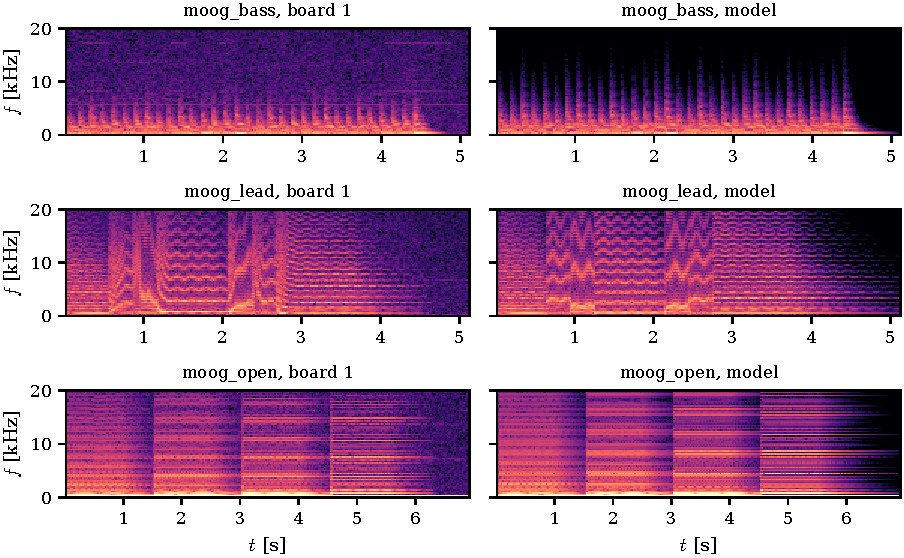
\includegraphics[width=0.85\textwidth]{s9_hw.pdf}
\caption{Three-oscillator test tunes on board~1 (left) and in the behavioural model (right).}\label{fig:s9hwtakes}
\end{figure}

\subsection{Bench tests of the voice bus}
\file{tools/bustest.py} runs the bus tests against the bench controller and one card. Each test prints PASS / FAIL
with the numbers it checked (Table~\ref{tab:bustest}); on the bench all pass at \SI{1}{Mbaud}, and also at
\SI{2}{Mbaud}.

\begin{table}[htbp]
\centering\small
\caption{Bus bench tests (\file{tools/bustest.py}).}\label{tab:bustest}
\begin{tabularx}{\textwidth}{@{}l X@{}}
\toprule
Test & Checks \\
\midrule
\texttt{enum} & enumeration state, HELLO with the chip ID, STATUS ``synced'' \\
\texttt{notes} & program change, note on / off, a phrase without CRC, late or slip errors \\
\texttt{patch} & patch slots and PATCH\_SELECT; modal strikes without late ticks \\
\texttt{ctrl} & CTRL (bend, wheel, expression) and PARAM reach the voice \\
\texttt{crc} & a corrupted packet is rejected and counted; a damaged packet loses only itself \\
\texttt{repair} & a lost NOTE\_ON is restored by VOICE\_STATE \\
\texttt{late} & late events run at once, far events are dropped, both counted \\
\texttt{config} & CONFIG changes $D$ \\
\texttt{sync} & SYNC gaps of several frames: bridging, muting, relock \\
\texttt{reset} & a card reset over SWIO is found and configured again \\
\texttt{counters} & the card's counters and STATUS, the controller's status line \\
\texttt{carrier}, \texttt{latency} & (oscilloscope) the DAC carrier with and without a DAC patch; latency against $D$ and $L$ \\
\texttt{stress}, \texttt{load} & dense traffic for \SI{20}{s}; the 8-voice load test (Section~\ref{sec:load}) \\
\bottomrule
\end{tabularx}
\end{table}

\subsection{Eight voices with one card (load test)}\label{sec:load}
The load test (\file{docs/bus.md} 9.5) emulates a full instrument with the bench hardware. The bench controller treats
voices 1--7 as populated (no HELLO expected) and sends all their traffic; the card is voice 0 and must discard the
rest. Notes are allocated as in \file{docs/midi.md} (one poly part) or go to 8 single-voice parts (MIDI channel $k$
$\to$ voice $k$). A generator in the controller plays chords and controller sweeps through the same MIDI path, and the
refreshes cover all 8 voices. Unless stated: \SI{1}{Mbaud}, $D = 4$, $L = 2$, the card on a two-oscillator DAC patch.

\paragraph{Bus.} The peak bytes per frame equal the computed sizes. A frame carries 88 bytes of events after FRAME,
and with $L = 2$ there is no slack: anything that does not fit the next frame is late at the cards by whole frames
(Table~\ref{tab:loadburst}). Per-voice records halve chords and refreshes.

\begin{table}[htbp]
\centering\small
\caption{Load test: bursts from one MIDI command (one execution frame), \file{docs/bus.md} 9.5.}\label{tab:loadburst}
\begin{tabularx}{\textwidth}{@{}X r r l l@{}}
\toprule
Burst & Bytes & Frames & Late at $L = 2$ & \shortstack[l]{Per-voice records:\\bytes, late} \\
\midrule
chord of 8 & 87 & 1 & 0 & 45, 0 \\
legato chord change (8 NOTE\_OFF, 8 NOTE\_ON) & 143 & 2 & 5 packets by 1 frame & 52, 0 \\
chord + bend, wheel, cutoff, one part & 114 & 2 & 3 by 1 & 72, 0 \\
chord + bend, wheel, cutoff, 8 parts & 303 & 4 & 24 by up to 3 & 114, 1 by 1 \\
VOICE\_STATE refresh, 8 voices & 1.5 / frame & & & 0.6 / frame \\
PATCH\_DATA, 8 values, one every 16 frames & 1.5 / frame & & & \\
\bottomrule
\end{tabularx}
\end{table}

Sustained traffic on 8 single-voice parts (chords every 250 frames, bend, wheel and cutoff on every part every $N$
frames) saturates the bus at about 86 bytes per frame: the backlog then grows without limit (late by up to 16 frames)
and the refreshes, which only use idle room, stop (Table~\ref{tab:loadsust}). Two controller-side measures help:
\begin{itemize}
  \item \textbf{Notes ahead of controllers (V\_PRIO):} two queues in the controller; CTRL and PARAM wait behind notes.
    No protocol change, and no note is late under any controller load.
  \item \textbf{Per-voice records:} the same events in fewer bytes; saturation only at 24\,000 events per second.
\end{itemize}
One poly part, the default setup, needs little: chords with the three controllers every 5 frames take 14 bytes per
frame, nothing late.

\begin{table}[htbp]
\centering\small
\caption{Load test: sustained traffic, 8 single-voice parts, late packets per \SI{5}{s} (\file{docs/bus.md}
9.5).}\label{tab:loadsust}
\setlength{\tabcolsep}{4pt}
\begin{tabular}{@{}r r r r r r l@{}}
\toprule
\shortstack[r]{$N$\\(events/s)} & \shortstack[r]{Bytes\\per frame} & Budget & \shortstack[r]{Late\\$L = 2$} &
\shortstack[r]{Late\\$L = 3$} & \shortstack[r]{V\_PRIO:\\notes late} & \shortstack[l]{Per-voice records:\\bytes per
frame, late} \\
\midrule
8 (3000) & 35 & 25\,\% & 9\,495 & 3\,825 & 0 & 16, 5 \\
4 (6000) & 62 & 50\,\% & 18\,993 & 7\,650 & 0 & 25, 10 \\
3 (8000) & 79 & 66\,\% & 25\,489 & 10\,374 & 0 & 30, 7 \\
2 (12000) & 86, saturated & 98\,\% & 45\,148 & 45\,124 & 0 & 42, 0 \\
1 (24000) & 86, saturated & 98\,\% & 45\,240 & & 0 & 75, saturated \\
\bottomrule
\end{tabular}
\end{table}

\paragraph{Card.} The card's CPU broke first, not the bus. Parsing in the tick cost about 128 cycles per byte (COBS,
CRC, then the address check; the V006 runs from flash with 2 wait states), for foreign bytes as for its own. Under
71 bytes per frame of foreign traffic a two-oscillator patch missed 1297 DAC buffer halves in \SI{10}{s}. Two parser
changes fixed that (Table~\ref{tab:loadcard}):
\begin{itemize}
  \item \textbf{Early discard:} packets for other cards are dropped at their dst byte, before the CRC, and the rest is
    skipped to the next 0x00 at memory speed;
  \item \textbf{In-place decoder:} the COBS decoder runs over the RX ring in place with its state in registers (an
    87-byte burst: 11.1\,k $\to$ 5.2\,k cycles).
\end{itemize}
The three-oscillator patch still misses halves. As one of 8 poly voices (14 bytes per frame) the two-oscillator and
the modal patches miss nothing, the three-oscillator patch 18--372 halves in \SI{10}{s}. The tick without replies takes
7\,k cycles without traffic and 9\,k under this load; the free stack was at least 156 bytes.

\paragraph{After the render rewrite} (2026-10-20, Section~\ref{sec:cpu}) no patch misses a half in any of these cases
(Table~\ref{tab:loadrw}), and the free stack is 656--680 bytes. Re-run on the final build: \texttt{bustest.py all}
17 of 17, \texttt{stress --progs 17} 0 missed (slack 157 periods), \texttt{load --voices 8} 0 underruns. The occasional
half counted as missed at a patch change was a counting artefact (a render preempted by the DAC restart and checked
against the new ring) and is no longer counted.

\begin{table}[htbp]
\centering\small
\caption{Load test: DAC buffer halves missed in \SI{10}{s} under 71 bytes per frame of foreign traffic (\file{docs/bus.md}
9.5).}\label{tab:loadcard}
\setlength{\tabcolsep}{4pt}
\begin{tabularx}{\textwidth}{@{}X r r r r@{}}
\toprule
Patch & No traffic: missed, slack & Before & Early discard & + in-place parser \\
\midrule
two oscillators (lead\_dac) & 0, 38--43 periods & 1\,297 & 0 & 0 \\
modal (kettle) & 0, 85 & 0 & 0 & 0 \\
three oscillators (moog\_bass) & 1--3, 4--11 & 6\,263 & 2\,231 & 1\,003--1\,748 \\
no DAC (init) & -- & 0 & 0 & 0 \\
Parser cycles per tick: mean, longest & 1.0\,k, 3.2\,k & 8.8\,k, 11.7\,k & 4.9\,k, 6.6\,k & 3.0--4.1\,k, 5.8\,k \\
\bottomrule
\end{tabularx}
\end{table}

\begin{table}[htbp]
\centering\small
\caption{Load test before and after the render rewrite: missed halves in \SI{10}{s} (stress: \SI{20}{s}) and the
least slack in carrier periods (after: the smallest of three runs; \file{docs/bus.md} 9.5).}\label{tab:loadrw}
\setlength{\tabcolsep}{4pt}
\begin{tabularx}{\textwidth}{@{}X l l l l@{}}
\toprule
Patch & No traffic & Foreign, 71\,B/frame & One of 8 poly voices & \texttt{stress --progs 17} \\
\midrule
lead\_dac (2 osc) & 0, 22 $\to$ 0, 175 & 0, 12 $\to$ 0, 161 & 0, 23 $\to$ 0, 164 & -- \\
kettle (modal) & 0, 85 $\to$ 0, 150 & 0, 71 $\to$ 0, 145 & 1, 16 $\to$ 0, 99 & -- \\
moog\_bass (3 osc) & 1, 4 $\to$ 0, 164 & 1\,796, 1 $\to$ 0, 154 & 33, 1 $\to$ 0, 157 & 188, 1 $\to$ 0, 157 \\
\bottomrule
\end{tabularx}
\end{table}

\paragraph{Latency under load.} On time, the latency does not depend on the load: $D$ frames plus one or two carrier
periods. A late event is late by whole frames (Table~\ref{tab:loadlat}).

\begin{table}[htbp]
\centering\small
\caption{Load test: latency from the SYNC edge of the execution frame to the note on PC2, 10 notes (\file{docs/bus.md}
9.5).}\label{tab:loadlat}
\begin{tabularx}{\textwidth}{@{}X l l@{}}
\toprule
Load & Mean & Spread \\
\midrule
none (5 notes) & 4.0088\,ms & 4.8\,\textmu s \\
7 parts, controllers every 3 frames (72 bytes/frame), the card's NOTE\_ON alone & 4.91\,ms: 4, 5 or 6\,ms & 2.0\,ms \\
the same, $L = 3$ & 4.41\,ms: 4 or 5\,ms & 1.0\,ms \\
the same, per-voice records (29 bytes/frame) & 4.0097\,ms & 5.4\,\textmu s \\
the same, V\_PRIO & 4.0096\,ms & 4.6\,\textmu s \\
the card's note in a chord of 8, the part's controllers every 3 frames & 4.0078\,ms & 6.7\,\textmu s \\
\bottomrule
\end{tabularx}
\end{table}

\paragraph{\SI{2}{Mbaud}.} With dividers 1.5 on the V006 and 36 on the V203 (both exact), \SI{2}{Mbaud} works on the
bench wiring: all 17 tests pass without CRC or UART errors. Bursts up to 190 bytes fit one frame, and the bus saturates
at 183 bytes per frame. A burst then reaches the cards in one tick, however (193 bytes: parser 13.3\,k, tick 17\,k
cycles), and the two-oscillator patch misses 90--440 halves per \SI{5}{s} even at a 35-byte average, against none at
\SI{1}{Mbaud}.

\paragraph{Conclusions} (\file{docs/bus.md} 9.5):
\begin{enumerate}
  \item notes ahead of controllers in the controller; coalescing queued controller values of the same voice and ID
    would also bound the backlog;
  \item per-voice records for chords and the VOICE\_STATE refresh (half the bytes, a legato chord change in one
    frame). For controllers on several parts they cost card CPU, because every addressed card decodes the whole packet;
  \item $L = 3$ where per-voice records are not used for legato chords and multi-part controllers (one frame of slack,
    7--8\,ms latency);
  \item \SI{1}{Mbaud} until the cards parse outside the tick;
  \item three-oscillator patches needed a cheaper render; done with the render rewrite (Table~\ref{tab:loadrw});
  \item the refresh rates can stay (1.5 bytes per frame for 8 voices).
\end{enumerate}
Only testable with 8 real cards: the electrical load on BCAST, RETURN and SYNC, the NRST enumeration, the alignment of
a chord across cards, and each card's CPU under its own and the other cards' traffic.

% =====================================================================================================================
\section{Manufacturing}\label{sec:mfg}

\subsection{Parts policy}
Both boards are assembled by JLCPCB from the \emph{Basic} and \emph{Promotional Extended} lists only, so no
extended-part fees arise. The part lists were taken from the JLCPCB parts API
(\file{parts/jlcpcb\_basic\_and\_promotional\_parts.csv}); \file{hw/lcsc.py} picks passives from it (Basic first, then
by stock), with voltage ratings of at least twice the working voltage and C0G wherever a capacitor is in the audio
path. Hand-soldered: the MCUs (own stock), connectors and headers, and parts missing from the lists (the polyfuse, the
host-port switch). The SPI flash is not fitted at first (own stock if fitted later). Table~\ref{tab:promo} lists
the Promotional Extended lines; on the voice card most of them are 0402 resistor values that are not Basic.

\textbf{Stock check (2026-10-20, live JLCPCB data for every BOM line of both boards):} all parts in stock in
quantity (the lowest, the SMAJ5.0A, at about 54\,000) except the SRV05-4A ESD array, which was down to 3; the design
now uses the SRV05-4 (C7420376, Promotional Extended, same package and pinout, about 42\,500 in stock).
\textbf{Fabrication data:} \file{hw/fab.py} writes the gerbers (four copper layers on both boards), the drill file and
the JLCPCB BOM and placement file per board (voice card: 49 BOM lines, 165 placements; backplane: 36 lines, 152
placements, the host port and the effects slot's two 0\,$\Omega$ included since 20 October; their parts reuse codes already on the board, all in stock). The placement rotations follow the usual KiCad-to-JLCPCB corrections; the polarised and multi-pin
parts (ICs, the TVS diode, the LEDs) are to be checked in JLCPCB's placement preview before ordering.

\begin{table}[htbp]
\centering\footnotesize
\caption{Promotional Extended lines (generated).}\label{tab:promo}
% generated by gen_tables.py -- do not edit
\begin{tabular}{@{}l l l l@{}}
\toprule
Board & LCSC & Part & Value \\
\midrule
voice card & C13320 & 0603WAF5104T5E & 5.1M \\
voice card & C13533 & CL05C331JB5NNNC & 330p \\
voice card & C23220 & 0603WAF6200T5E & 620 \\
voice card & C25750 & 0402WGF1203TCE & 120k \\
voice card & C25762 & 0402WGF1802TCE & 18k \\
voice card & C25769 & 0402WGF2402TCE & 24k \\
voice card & C25771 & 0402WGF2702TCE & 27k \\
voice card & C25790 & 0402WGF4703TCE & 470k \\
voice card & C25822 & 0603WAF6803T5E & 680k \\
voice card & C25862 & 0402WGF1201TCE & 1.2k \\
voice card & C25882 & 0402WGF2401TCE & 2.4k \\
voice card & C25918 & 0402WGF7501TCE & 7.5k \\
voice card & C25950 & 0603WAF1102T5E & 11k \\
voice card & C41375126 & BC847BS & BC847BS \\
voice card & C4197 & 0603WAF2403T5E & 240k \\
voice card & C7377 & MCP6002T-I/SN & MCP6002 \\
voice card & C89811 & NCD0603Y2 & yellow \\
\midrule
backplane & C20615829 & SRV05-4A & SRV05-4A \\
backplane & C2925443 & SMAJ5.0A & SMAJ5.0A \\
backplane & C7377 & MCP6002T-I/SN & MCP6002 \\
backplane & C89811 & NCD0603Y2 & yellow \\
\bottomrule
\end{tabular}

\end{table}

\subsection{BOM summary and cost}
\begin{table}[htbp]
\centering\small
\caption{BOM summary (generated from \file{hw/voice.py}, \file{hw/backplane.py} and the parts list). Cost: assembled
parts at the list unit prices, without PCB, assembly fees, MCUs and hand-soldered parts.}\label{tab:bomsum}
\begin{tabular}{@{}l r r@{}}
\toprule
& Voice card & Backplane \\
\midrule
Parts in the design & \statVoiceParts & \statBpParts \\
Assembled (JLCPCB) & \statVoiceAsm & \statBpAsm \\
BOM lines: Basic / Promotional & \statVoiceBasic\ / \statVoicePromo & \statBpBasic\ / \statBpPromo \\
Hand-soldered & \statVoiceHand & \statBpHand \\
Not fitted (DNP) & \statVoiceDnp & \statBpDnp \\
Test points & \statVoiceTp & \statBpTp \\
Assembled parts cost (USD) & \statVoiceCost & \statBpCost \\
\bottomrule
\end{tabular}
\end{table}
The assembled parts of 8 cards and one backplane cost about USD \statSystemCost\ at list prices. To this come the
hand-soldered parts (on the backplane about USD 3--6 without the MCU and the flash: sockets, USB connectors, jack,
headers, polyfuse; on each card the 2$\times$8 right-angle header and two 1$\times$3 headers), the MCUs from own stock,
the PCBs (both boards are in JLCPCB's smallest price class) and the order-level assembly fees, which dominate at small
quantities. The full BOMs are in Appendix~\ref{app:bom}.

\subsection{Fabrication data}
\file{hw/fab.py} (with \texttt{BOARD=backplane} for the backplane) writes the Gerber files of all copper layers plus
mask, paste, silkscreen and outline, the Excellon drill file, the BOM and the placement file with rotation offsets for
the SOT, SOIC and TSSOP packages, into \file{hw/<board>/production/}. Parts marked DNP or hand-soldered are excluded
from assembly. The placement preview on the JLCPCB order page must be checked for the SOT-23 / SOT-363 transistors,
the diodes and the LEDs.

% =====================================================================================================================
\section{Open points and risks}\label{sec:open}
\begin{itemize}
  \item \textbf{Nothing new is built yet.} The voice card and the backplane are simulated, drawn and routed (DRC clean);
    review and order are pending. The first step is one card at \SI{5}{V} on the bench, powered by the programmer (V2),
    before the backplane.
  \item \textbf{\SI{5}{V} core against the simulation.} Microchip's MCP6002 model lacks the input-stage transition and
    distortion detail. The INA inputs stay above the transition and the difference amplifiers below it by design;
    resonance, THD and offsets need the bench check on the first card.
  \item \textbf{Card CPU.} Resolved on the bench card by the render rewrite: every patch runs under 8-voice bus load
    without a missed half, three oscillators at 23\,\% CPU (Section~\ref{sec:cpu}). Remaining: the modal patch as one
    of 8 poly voices has the smallest margin (99 periods); the assembly loops are verified only by the card's render
    hashes; a patch change that preempts a render can glitch that one block (the oscillator buffer and the mallet table
    share memory). Each card's CPU under real 8-card traffic is to be confirmed in V4.
  \item \textbf{Bus lead $L = 2$ has no slack.} A frame carries 88 bytes of events; a legato chord change or
    controllers on 8 parts arrive late by whole frames, and a sustained load of about 86 bytes per frame saturates the
    bus. Recommended for the controller: notes ahead of controllers (two queues), coalescing of queued controller
    values, per-voice records for chords and the VOICE\_STATE refresh, and $L = 3$ where those are not used. To be
    confirmed with 8 real cards.
  \item \textbf{RAM and stack.} \SI{8}{KB} is tight: the card build uses about \SI{7.0}{KB} of static RAM and keeps
    650--680 bytes of stack free under bus load (about 340 with the console); the console captures shrank to 1280
    samples. Board~1's build (\SI{7.5}{KB} static RAM, about 700 bytes for the stack) is untested on hardware.
  \item \textbf{Firmware not yet written:} the controller firmware (USB host, allocation, patch storage, SWIO
    programmer; USB-MIDI + CDC device runs on the bench on USBFS and enumerated on USBD; a MIDI host on USBFS works in a
    self-loop, a real keyboard is untested); on the card PATCH\_DATA, CALIBRATE, the \SI{5}{V} calibration tables (the firmware and the model
    still use rev 0.1's data) and the dual-PWM ratio measurement.
  \item \textbf{HSI wander} between voices (0.35\,cent rms) may be audible on unison patches. The crystal-locked
    \SI{24}{MHz} CLK\_IN option removes it; its signal over about \SI{100}{mm} and 8 stubs, the V006's input level for an
    external clock and EMI near the ADC are unverified.
  \item \textbf{Carrier residue} from 8 unsynchronised cards could beat in the mixer; each card is at
    \statSelevenCarrier\,dB at its line out. To check in V4.
  \item \textbf{Steering-pair mismatch} clicks at the centre pan position (about \statSthirteenClick\,mV per mV). The
    BC847BS pairs are matched on one die; to be measured on the first card.
  \item \textbf{Backplane, unverified items:} the 74HC595 speed at \SI{3.3}{V} (written at \SI{9}{MHz}); a push-pull
    reset into a card (NRST is driven with no series resistor; the V006's default option bytes do make PD7 its NRST,
    verified 2026-10-20, Section~\ref{sec:srsorder}); USBD enumerating against a computer (its internal pull-up
    has so far only been shown against the V203's own host); the BY25D16 command set; the
    LTV-817S at \SI{31.25}{kbaud} and \SI{3.3}{V}; the card-plane offset and the socket rotation with the chosen
    headers.
  \item \textbf{Inrush and USB limits:} about \SI{1.8}{A} for a few milliseconds at plug-in, and about \SI{115}{mA}
    before configuration. Accepted; the soft start is a footprint (to simulate first, S14).
  \item \textbf{Summing band:} the one long break in the bottom ground pour; the alternative is a top-layer band with
    bridging resistors.
  \item \textbf{Mechanics:} card guides or an enclosure; the bulk capacitor height on the card (\SI{6}{mm} limit).
  \item \textbf{Assembly:} hand-soldered TSSOP-20 and LQFP-48; check for bridges (board~1 had one on PD4/PD5).
\end{itemize}

% =====================================================================================================================
\appendix
\section{Schematics}\label{app:sch}
The following pages reproduce the KiCad schematics (\file{docs/schematics/voice.pdf}, \statVoiceSheets\ sheets and
the root sheet, and \file{docs/schematics/backplane.pdf}, \statBpSheets\ sheets and the root sheet), scaled to A4. The
PDFs are vector graphics and can be zoomed.

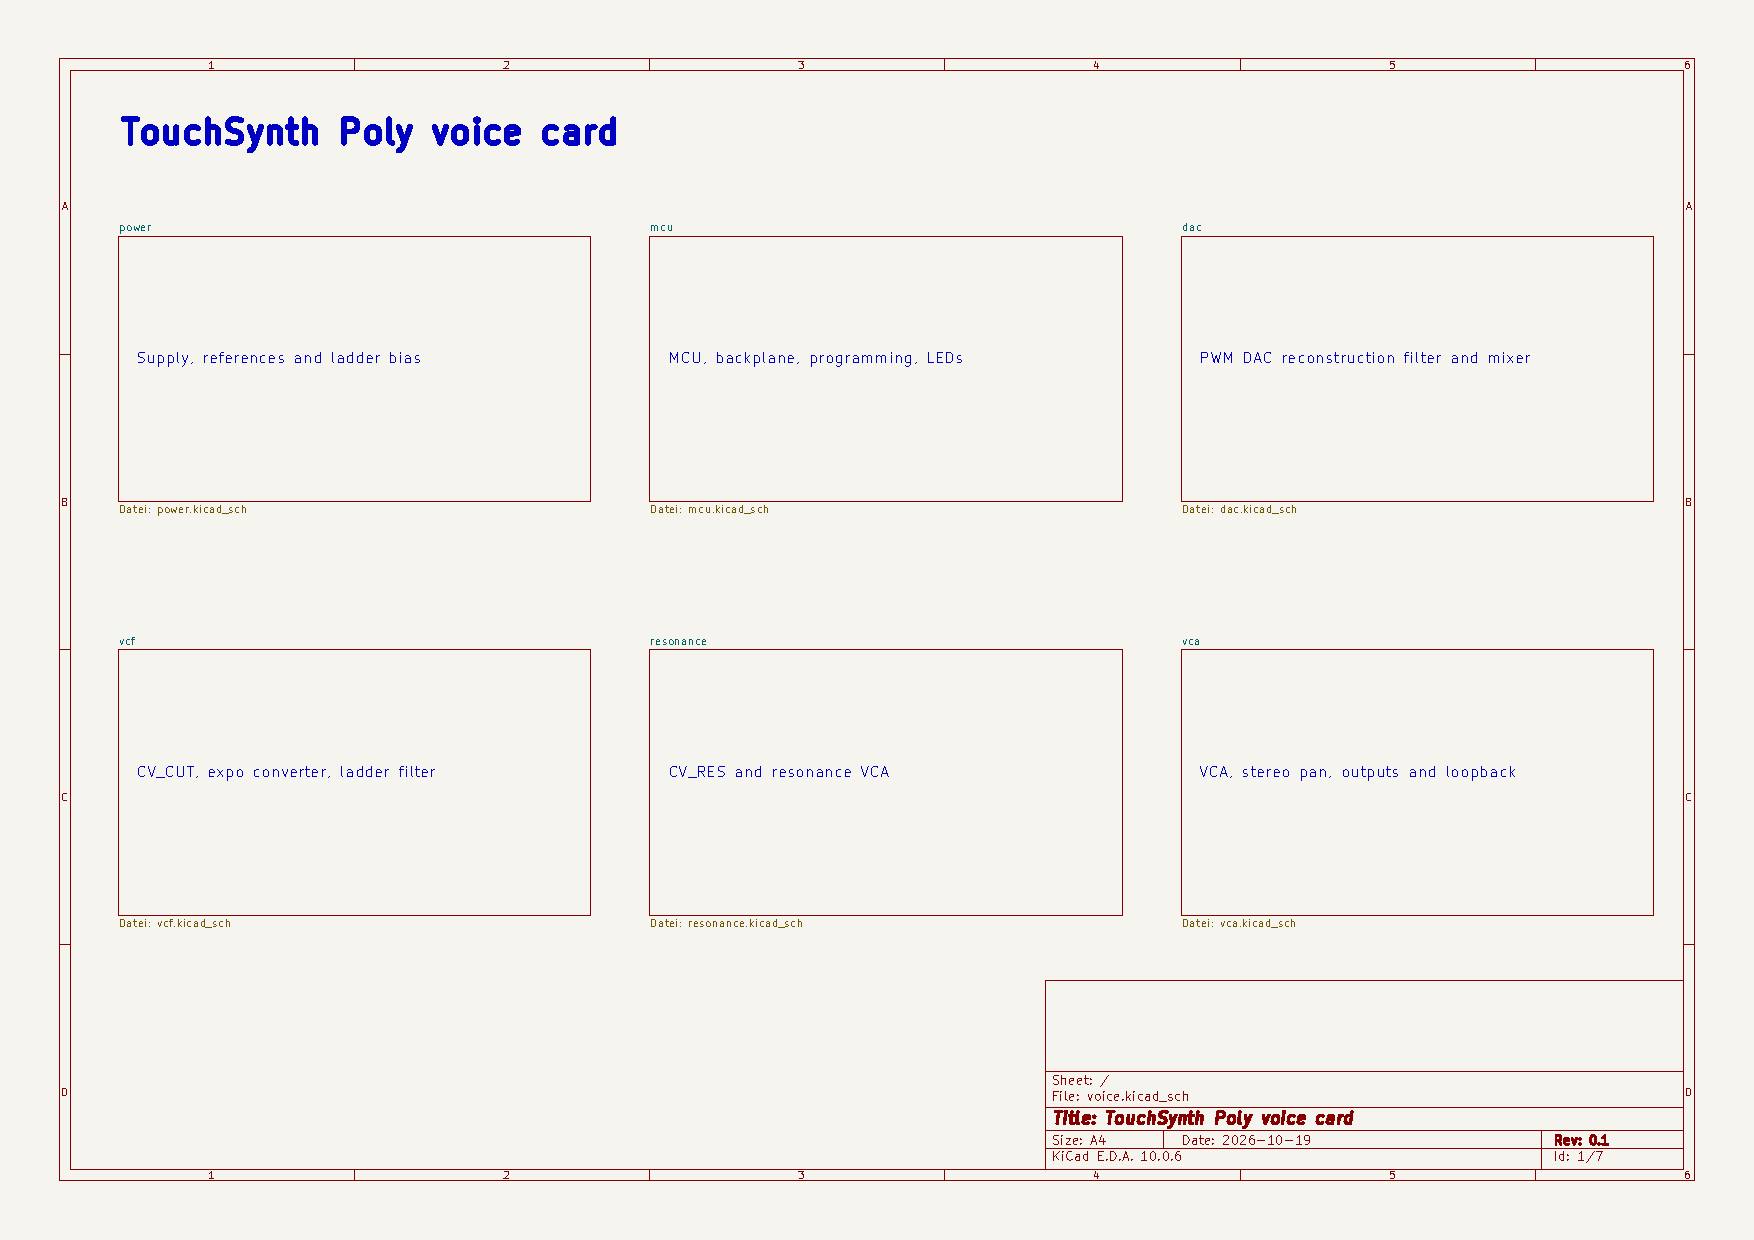
\includepdf[pages=-,landscape,fitpaper=false,scale=0.95,pagecommand={\thispagestyle{fancy}},
  addtotoc={1,subsection,2,{Voice card},app:schvoice}]{../schematics/voice.pdf}
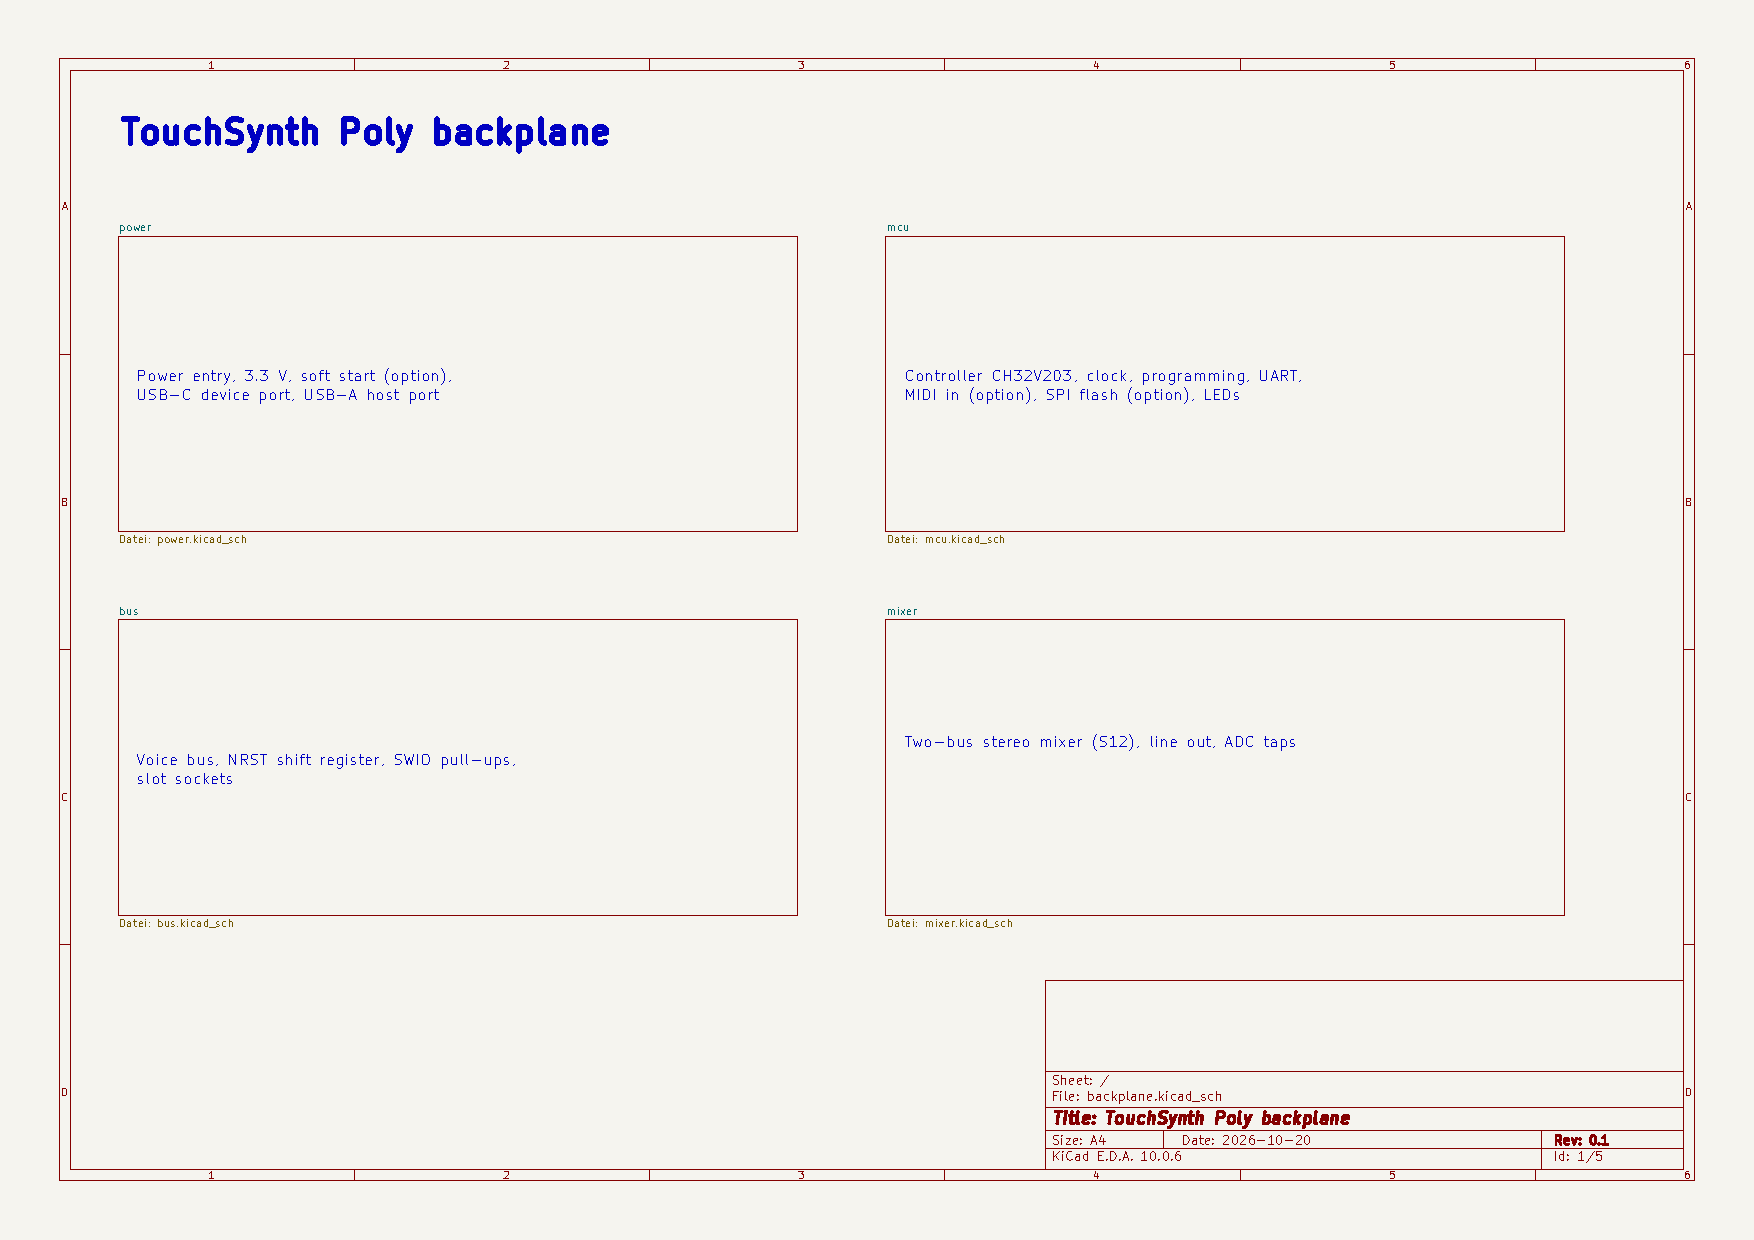
\includepdf[pages=-,landscape,fitpaper=false,scale=0.95,pagecommand={\thispagestyle{fancy}},
  addtotoc={1,subsection,2,{Backplane},app:schbp}]{../schematics/backplane.pdf}

\section{Bills of materials}\label{app:bom}
{\small% generated by gen_tables.py -- do not edit
\begin{longtable}{@{}l r l l l r >{\raggedright\arraybackslash}p{4.1cm}@{}}
\caption{Voice card: assembled parts (JLCPCB PCBA, top side). Unit prices from the JLCPCB parts list snapshot.}\label{tab:bomvoice}\\
\toprule Value & Qty & Package & LCSC & Library & USD/pc & Designators\\ \midrule\endfirsthead
\toprule Value & Qty & Package & LCSC & Library & USD/pc & Designators\\ \midrule\endhead
\bottomrule\endfoot
10k & 22 & 0402 & C25744 & Basic & 0.0034 & {\footnotesize R3, R5--R7, R31, R38, R39, R41, R42, R51, R52, R55--R58, R67, R68, R83, R85, R91, R93, R100}\\
1k & 11 & 0402 & C11702 & Basic & 0.0018 & {\footnotesize R2, R20, R21, R32, R37, R44, R48, R60, R64, R70, R71}\\
4.7k & 11 & 0402 & C25900 & Basic & 0.0027 & {\footnotesize R33, R45, R46, R53, R54, R61, R62, R76--R79}\\
100k & 6 & 0402 & C25741 & Basic & 0.0025 & {\footnotesize R15, R17, R40, R43, R90, R98}\\
1.5k & 5 & 0402 & C25867 & Basic & 0.0029 & {\footnotesize R9--R12, R35}\\
100 & 5 & 0402 & C25076 & Basic & 0.0012 & {\footnotesize R14, R16, R18, R89, R97}\\
33k & 5 & 0402 & C25779 & Basic & 0.0058 & {\footnotesize R69, R87, R88, R95, R96}\\
30k & 4 & 0603 & C22984 & Basic & 0.0050 & {\footnotesize R84, R86, R92, R94}\\
11k & 2 & 0603 & C25950 & Promo & 0.0019 & {\footnotesize R26, R27}\\
15k & 2 & 0402 & C25756 & Basic & 0.0016 & {\footnotesize R4, R101}\\
240k & 2 & 0603 & C4197 & Promo & 0.0049 & {\footnotesize R30, R66}\\
3k & 2 & 0603 & C4211 & Basic & 0.0023 & {\footnotesize R63, R80}\\
1.2k & 1 & 0402 & C25862 & Promo & 0.0023 & {\footnotesize R65}\\
120k & 1 & 0402 & C25750 & Promo & 0.0012 & {\footnotesize R50}\\
12k & 1 & 0402 & C25752 & Basic & 0.0018 & {\footnotesize R47}\\
18k & 1 & 0402 & C25762 & Promo & 0.0014 & {\footnotesize R34}\\
2.2k & 1 & 0402 & C25879 & Basic & 0.0053 & {\footnotesize R19}\\
2.4k & 1 & 0402 & C25882 & Promo & 0.0017 & {\footnotesize R74}\\
22 & 1 & 0402 & C25092 & Basic & 0.0027 & {\footnotesize R1}\\
22k & 1 & 0402 & C25768 & Basic & 0.0024 & {\footnotesize R59}\\
24k & 1 & 0402 & C25769 & Promo & 0.0046 & {\footnotesize R82}\\
27k & 1 & 0402 & C25771 & Promo & 0.0017 & {\footnotesize R81}\\
3.3k & 1 & 0402 & C25890 & Basic & 0.0035 & {\footnotesize R13}\\
3.6k & 1 & 0603 & C22980 & Basic & 0.0019 & {\footnotesize R49}\\
470k & 1 & 0402 & C25790 & Promo & 0.0030 & {\footnotesize R36}\\
5.1M & 1 & 0603 & C13320 & Promo & 0.0022 & {\footnotesize R73}\\
620 & 1 & 0603 & C23220 & Promo & 0.0020 & {\footnotesize R8}\\
680k & 1 & 0603 & C25822 & Promo & 0.0015 & {\footnotesize R72}\\
7.5k & 1 & 0402 & C25918 & Promo & 0.0021 & {\footnotesize R75}\\
1\textmu{} & 12 & 0402 & C52923 & Basic & 0.0099 & {\footnotesize C4, C5, C8, C9, C16, C21, C34, C39--C43}\\
100n & 10 & 0402 & C1525 & Basic & 0.0045 & {\footnotesize C7, C15, C22, C24, C30, C31, C36, C44, C46, C49}\\
10\textmu{} & 6 & 0402 & C15525 & Basic & 0.0255 & {\footnotesize C6, C12--C14, C45, C47}\\
10n & 4 & 0402 & C15195 & Basic & 0.0050 & {\footnotesize C26--C29}\\
100\textmu{} & 3 & 1206 & C15008 & Basic & 0.1253 & {\footnotesize C1--C3}\\
330p & 3 & 0402 & C13533 & Promo & 0.0081 & {\footnotesize C18--C20}\\
33n & 3 & 0603 & C21117 & Basic & 0.0106 & {\footnotesize C23, C32, C37}\\
10\textmu{} & 2 & 0603 & C19702 & Basic & 0.0319 & {\footnotesize C10, C11}\\
1n & 2 & 0402 & C1523 & Basic & 0.0042 & {\footnotesize C25, C48}\\
22n & 2 & 0402 & C1532 & Basic & 0.0091 & {\footnotesize C33, C38}\\
4.7\textmu{} & 1 & 0402 & C23733 & Basic & 0.0166 & {\footnotesize C35}\\
red & 2 & 0603 & C2286 & Basic & 0.0075 & {\footnotesize D2, D4}\\
B5819W & 1 & SOD-123 & C8598 & Basic & 0.0280 & {\footnotesize D1}\\
yellow & 1 & 0603 & C89811 & Promo & 0.0195 & {\footnotesize D3}\\
BC847BS & 10 & SOT-363 & C41375126 & Promo & 0.0281 & {\footnotesize Q1--Q6, Q8, Q10--Q12}\\
MMBT3904 & 2 & SOT-23 & C20526 & Basic & 0.0115 & {\footnotesize Q7, Q9}\\
MCP6002 & 4 & SOIC-8 & C7377 & Promo & 0.2865 & {\footnotesize U3, U5--U7}\\
CJ431 & 1 & SOT-23 & C3113 & Basic & 0.0411 & {\footnotesize U2}\\
LM324 & 1 & SOIC-14 & C71035 & Basic & 0.1658 & {\footnotesize U8}\\
XC6206P332MR & 1 & SOT-23 & C5446 & Basic & 0.1425 & {\footnotesize U1}\\
\midrule
\multicolumn{2}{@{}l}{165 parts} & \multicolumn{3}{l}{49 BOM lines} & 3.01 & per board (parts only)\\
\end{longtable}
}
{\small% generated by gen_tables.py -- do not edit
\begin{longtable}{@{}l l l l >{\raggedright\arraybackslash}p{6.4cm}@{}}
\caption{Voice card: hand-soldered and not-fitted parts (test points not listed).}\label{tab:handvoice}\\
\toprule Ref & Value & Package & Status & Note\\ \midrule\endfirsthead
\toprule Ref & Value & Package & Status & Note\\ \midrule\endhead
\bottomrule\endfoot
U4 & CH32V006F8P7 & TSSOP-20 & hand-soldered & {\footnotesize own stock, hand-soldered; TIM1\_RM 0010, TIM2\_RM 010 (PC5 = TIM2 CH1: pan); PA4 bonded to PD7: never an output}\\
J1 & BACKPLANE & header 2$\times$8, R/A & hand-soldered & {\footnotesize 2x8 right-angle header, card underside edge; pin 6 = AUDIO\_GND: route from the line-out ground}\\
C17 & 100n & 0402 & not fitted & {\footnotesize NRST filter (option)}\\
J2 & SWIO & header 1$\times$3, R/A & hand-soldered & {\footnotesize WCH-LinkE: 5V, SWIO, GND (right-angle, debug edge)}\\
J3 & LINE OUT & header 1$\times$3, R/A & hand-soldered & {\footnotesize right-angle, debug edge: L, R, GND}\\
R22 & 0 & 0402 & not fitted & {\footnotesize external 24 MHz clock from the backplane (TIM3 CH4; fallback, spec 6)}\\
R23 & 10k & 0402 & not fitted & {\footnotesize self-test: ladder bias VB0 to ADC A0}\\
R24 & 10k & 0402 & not fitted & {\footnotesize self-test: analog rail / 2 to ADC A3}\\
R25 & 10k & 0402 & not fitted & {\footnotesize self-test divider}\\
R28 & 1M & 0402 & not fitted & {\footnotesize dual-PWM option}\\
R29 & 330k & 0402 & not fitted & {\footnotesize dual-PWM option}\\
R99 & 10k & 0402 & not fitted & {\footnotesize option: R into the loopback (L + R summed at PC4)}\\
\end{longtable}
}
{\small% generated by gen_tables.py -- do not edit
\begin{longtable}{@{}l r l l l r >{\raggedright\arraybackslash}p{4.1cm}@{}}
\caption{Backplane: assembled parts (JLCPCB PCBA, top side). Unit prices from the JLCPCB parts list snapshot.}\label{tab:bombp}\\
\toprule Value & Qty & Package & LCSC & Library & USD/pc & Designators\\ \midrule\endfirsthead
\toprule Value & Qty & Package & LCSC & Library & USD/pc & Designators\\ \midrule\endhead
\bottomrule\endfoot
56k & 32 & 0603 & C23206 & Basic & 0.0027 & {\footnotesize R31--R62}\\
10k & 8 & 0603 & C25804 & Basic & 0.0018 & {\footnotesize R18, R21--R24, R30, R64, R66}\\
20k & 4 & 0603 & C4184 & Basic & 0.0023 & {\footnotesize R67--R70}\\
27k & 3 & 0603 & C22967 & Basic & 0.0046 & {\footnotesize R65, R74, R78}\\
33 & 3 & 0603 & C23140 & Basic & 0.0025 & {\footnotesize R26, R28, R29}\\
0 & 2 & 0603 & C21189 & Basic & 0.0023 & {\footnotesize R7, R8}\\
100k & 2 & 0603 & C25803 & Basic & 0.0031 & {\footnotesize R72, R76}\\
15k & 2 & 0603 & C22809 & Basic & 0.0029 & {\footnotesize R73, R77}\\
1k & 2 & 0603 & C21190 & Basic & 0.0026 & {\footnotesize R25, R27}\\
1k & 2 & 4x0603 & C20197 & Basic & 0.0171 & {\footnotesize RN1, RN2}\\
220 & 2 & 0603 & C22962 & Basic & 0.0034 & {\footnotesize R71, R75}\\
5.1k & 2 & 0603 & C23186 & Basic & 0.0015 & {\footnotesize R5, R6}\\
0 & 1 & 1206 & C17888 & Basic & 0.0085 & {\footnotesize R2}\\
2.2k & 1 & 0603 & C4190 & Basic & 0.0018 & {\footnotesize R1}\\
22k & 1 & 0603 & C31850 & Basic & 0.0041 & {\footnotesize R10}\\
33k & 1 & 0603 & C4216 & Basic & 0.0022 & {\footnotesize R11}\\
47 & 1 & 0603 & C23182 & Basic & 0.0040 & {\footnotesize R63}\\
10\textmu{} & 24 & 0805 & C15850 & Basic & 0.0788 & {\footnotesize C30--C53}\\
10\textmu{} & 14 & 0603 & C19702 & Basic & 0.0319 & {\footnotesize C1, C4, C22--C29, C55, C56, C62, C64}\\
100n & 9 & 0603 & C14663 & Basic & 0.0122 & {\footnotesize C11--C14, C16, C17, C20, C21, C57}\\
47p & 4 & 0603 & C1671 & Basic & 0.0064 & {\footnotesize C58--C61}\\
1\textmu{} & 3 & 0603 & C15849 & Basic & 0.0752 & {\footnotesize C2, C3, C15}\\
30p & 2 & 0603 & C1658 & Basic & 0.0080 & {\footnotesize C18, C19}\\
330p & 2 & 0603 & C1664 & Basic & 0.0179 & {\footnotesize C63, C65}\\
47\textmu{} & 2 & 1206 & C96123 & Basic & 0.2428 & {\footnotesize C6, C7}\\
22\textmu{} & 1 & 0805 & C45783 & Basic & 0.2199 & {\footnotesize C54}\\
SMAJ5.0A & 1 & SMA & C2925443 & Promo & 0.0387 & {\footnotesize D1}\\
red & 1 & 0603 & C2286 & Basic & 0.0075 & {\footnotesize D2}\\
yellow & 1 & 0603 & C89811 & Promo & 0.0195 & {\footnotesize D6}\\
BLM18PG121SN1D & 1 & 0603 & C14709 & Basic & 0.0146 & {\footnotesize FB1}\\
RESET & 1 & TS-1187A & C318884 & Basic & 0.0205 & {\footnotesize SW1}\\
74HC595D & 1 & SOIC-16 & C5947 & Basic & 0.1152 & {\footnotesize U6}\\
MCP6002 & 1 & SOIC-8 & C7377 & Promo & 0.2865 & {\footnotesize U8}\\
SRV05-4A & 1 & SOT-23-6 & C20615829 & Promo & 0.0470 & {\footnotesize U3}\\
XC6206P332MR & 1 & SOT-23 & C5446 & Basic & 0.1425 & {\footnotesize U2}\\
8MHz & 1 & 5032 & C115962 & Basic & 0.2446 & {\footnotesize Y1}\\
\midrule
\multicolumn{2}{@{}l}{140 parts} & \multicolumn{3}{l}{36 BOM lines} & 4.61 & per board (parts only)\\
\end{longtable}
}
{\small% generated by gen_tables.py -- do not edit
\begin{longtable}{@{}l l l l >{\raggedright\arraybackslash}p{6.4cm}@{}}
\caption{Backplane: hand-soldered and not-fitted parts (test points not listed).}\label{tab:handbp}\\
\toprule Ref & Value & Package & Status & Note\\ \midrule\endfirsthead
\toprule Ref & Value & Package & Status & Note\\ \midrule\endhead
\bottomrule\endfoot
J4 & EXT 5V & header 1$\times$2 & hand-soldered & {\footnotesize external 5 V, $>$= 1 A adapter (hand-soldered)}\\
JP1 & SUPPLY & header 1$\times$3 & hand-soldered & {\footnotesize 1-2: USB-C, 2-3: external 5 V (no diode drop)}\\
F1 & 0.75A & 1206 & hand-soldered & {\footnotesize PTC, I\_hold 0.75 A, I\_trip 1.5 A (e.g. Bourns MF-MSMF075), hand-soldered: not on the lists}\\
Q1 & AO3401A & SOT-23 & not fitted & {\footnotesize P-channel soft start, about 40 ms ramp (hand estimate; simulate first: S14)}\\
R3 & 1M & 0603 & not fitted & {\footnotesize soft start R\_GS}\\
R4 & 220k & 0603 & not fitted & {\footnotesize soft start R\_G}\\
C5 & 100n & 0603 & not fitted & {\footnotesize soft start C\_GD}\\
J1 & USB-C & USB-C 16P & hand-soldered & {\footnotesize GCT USB4105, hand-soldered}\\
R9 & 1.5k & 0603 & not fitted & {\footnotesize D+ pull-up option (the USBD pull-up is expected inside)}\\
U4 & TPS2051C & SOT-23-5 & not fitted & {\footnotesize 0.5 A current-limited switch, enable active high, open-drain fault; hand-soldered: not on the lists}\\
C8 & 1\textmu{} & 0603 & not fitted & {\footnotesize host switch input}\\
C9 & 47\textmu{} & 1206 & not fitted & {\footnotesize host VBUS}\\
C10 & 47\textmu{} & 1206 & not fitted & {\footnotesize host VBUS}\\
R12 & 100k & 0603 & not fitted & {\footnotesize host port off until the firmware enables it}\\
R13 & 10k & 0603 & not fitted & {\footnotesize fault pull-up}\\
R14 & 1k & 0603 & not fitted & {\footnotesize fault LED series}\\
D3 & red & 0603 & not fitted & {\footnotesize host port fault}\\
R15 & 2.2k & 0603 & not fitted & {\footnotesize host power LED series}\\
D4 & yellow & 0603 & not fitted & {\footnotesize host port powered}\\
J2 & USB-A & USB-A & not fitted & {\footnotesize right-angle THT receptacle, hand-soldered}\\
U5 & SRV05-4A & SOT-23-6 & not fitted & {\footnotesize ESD on the host D-, D+}\\
R16 & 15k & 0603 & not fitted & {\footnotesize host pull-down option (USBFS pull-downs expected inside)}\\
R17 & 15k & 0603 & not fitted & {\footnotesize host pull-down option}\\
U1 & CH32V203C8T6 & LQFP-48 & hand-soldered & {\footnotesize own stock, hand-soldered; SPI1 remap 1 (PA15/PB3/PB4/PB5); TIM3 CH4 (PB1) = 24 MHz CLK option}\\
J5 & SWD & header 1$\times$4 & hand-soldered & {\footnotesize WCH-LinkE: 3V3, SWDIO, SWCLK, GND}\\
JP2 & BOOT0 & header 1$\times$3 & hand-soldered & {\footnotesize 1-2: system bootloader (USART1 / USB), open or 2-3: run from flash}\\
J6 & UART & header 1$\times$3 & hand-soldered & {\footnotesize USART1: GND, TX (PA9), RX (PA10); 5 V adapters are fine (FT)}\\
J7 & MIDI IN & header 1$\times$3 & not fitted & {\footnotesize DIN pin 4, DIN pin 5, shield (panel jack on wires)}\\
R19 & 220 & 0603 & not fitted & {\footnotesize MIDI loop series}\\
U9 & LTV-817S & SMDIP-4 & not fitted & {\footnotesize slow for 31.25 kbaud at 3.3 V (unverified); 6N138 by hand if needed}\\
D5 & 1N4148W & SOD-123 & not fitted & {\footnotesize opto LED reverse protection}\\
R20 & 1k & 0603 & not fitted & {\footnotesize opto collector pull-up}\\
JP3 & MIDI & header 1$\times$2 & not fitted & {\footnotesize fit only for DIN MIDI: USART1 RX then not available to J6}\\
U7 & W25Q128JVSIQ & SOIC-8 & not fitted & {\footnotesize SOP-8 208 mil: W25Q128JVSIQ or BY25D16ASTIG (own stock), hand-soldered later}\\
J3 & LINE OUT & 3.5 mm jack & hand-soldered & {\footnotesize CUI SJ1-3523N, hand-soldered}\\
J10--J17 & SLOT 1--8 & socket 2$\times$8 & hand-soldered & {\footnotesize voice card socket, hand-soldered, 2$\times$8 female, vertical}\\
\end{longtable}
}

\section{Reproducing the design}
\begin{footnotesize}
\begin{verbatim}
# simulations (each writes docs/results/*.csv and docs/figures/*)
cd sim/s10_5v && python s10_5v.py    # likewise s11_recon, s12_mixer --bus2, s13_pan
# schematics and checks (BOARD=voice is the default)
cd hw && python gen_sch2.py && python check_netlist.py && python check_sim.py
cd hw && BOARD=backplane python gen_sch2.py && BOARD=backplane python check_sim.py
# PCB (KiCad Python), fabrication data, figures
cd hw && <KiCad python> gen_pcb.py ...   # backplane: gen_pcb_bp.py
cd hw && python fab.py && BOARD=backplane python fab.py
cd hw && python pcb_figures.py && BOARD=backplane python pcb_figures.py
# firmware (WSL)
cd firmware/voice && make BOARD=card TARGET_MCU=CH32V006   # bench: BUS_TX_PP=1
cd firmware/bench_ctrl && make
# bench tests
cd tools && python3 bustest.py all && python3 bustest.py latency
# this report (WSL)
cd docs/report && python3 gen_tables.py
latexmk -pdf touchsynth_poly_report.tex
\end{verbatim}
\end{footnotesize}

\end{document}
